\documentclass[a4paper,twoside]{article}
\usepackage[T1]{fontenc}
\usepackage[bahasa]{babel}
\usepackage{graphicx}
\usepackage{graphics}
\usepackage{float}
\usepackage[cm]{fullpage}
\pagestyle{myheadings}
\usepackage{etoolbox}
\usepackage{setspace} 
\usepackage{lipsum} 


\usepackage{xcolor} 
\definecolor{mygray}{gray}{0.80}
% for 'lightgray' color

\newcommand{\myparagraph}[1]{\paragraph{#1}\mbox{}\\}

\setlength{\headsep}{30pt}
\usepackage[inner=2cm,outer=2.5cm,top=2.5cm,bottom=2cm]{geometry} %margin
\graphicspath{ {./Gambar/} }
% \pagestyle{empty}

\usepackage{listings}%untuk penulisan source code
%listing khusus untuk penulisan kode program, menggunakan font Bera Mono
\lstset{numbers=left,stepnumber=1, numbersep=5pt, frame=leftline,
	tabsize=4, breaklines=true, basicstyle=\fontfamily{fvm}\selectfont\tiny, 
	commentstyle=\itshape\color{gray}, keywordstyle=\bfseries\color{blue}, 
	stringstyle=\color{orange},
	literate={-}{-}1{-\,-}{--}1
} 



\makeatletter
\renewcommand{\@maketitle} {\begin{center} {\LARGE \textbf{ \textsc{\@title}} \par} \bigskip {\large \textbf{\textsc{\@author}} }\end{center} }
\renewcommand{\thispagestyle}[1]{}
\markright{\textbf{\textsc{Laporan Perkembangan Pengerjaan Skripsi\textemdash Sem. Ganjil 2019/2020}}}

\onehalfspacing

\begin{document}
	
	\title{\@judultopik}
	\author{\nama \textendash \@npm} 
	
	%ISILAH DATA BERIKUT INI:
	\newcommand{\nama}{Hapsari Laksmi W}
	\newcommand{\@npm}{2015730037}
	\newcommand{\tanggal}{11/14/2019} %Tanggal pembuatan dokumen
	\newcommand{\@judultopik}{Migrasi Zurb Foundation ke Bootstrap 4} % Judul/topik anda
	\newcommand{\kodetopik}{PAN4791}
	\newcommand{\jumpemb}{1} % Jumlah pembimbing, 1 atau 2
	\newcommand{\pembA}{Pascal Alfadian .N}
	\newcommand{\pembB}{-}
	\newcommand{\semesterPertama}{47 - Ganjil 19/20} % semester pertama kali topik diambil, angka 1 dimulai dari sem Ganjil 96/97
	\newcommand{\lamaSkripsi}{1} % Jumlah semester untuk mengerjakan skripsi s.d. dokumen ini dibuat
	\newcommand{\kulPertama}{Skripsi 1} % Kuliah dimana topik ini diambil pertama kali
	\newcommand{\tipePR}{B} % tipe progress report :
	% A : dokumen pendukung untuk pengambilan ke-2 di Skripsi 1
	% B : dokumen untuk reviewer pada presentasi dan review Skripsi 1
	% C : dokumen pendukung untuk pengambilan ke-2 di Skripsi 2
	
	% Dokumen hasil template ini harus dicetak bolak-balik !!!!
	
	\maketitle
	
	\pagenumbering{arabic}
	
	\section{Data Skripsi} %TIDAK PERLU MENGUBAH BAGIAN INI !!!
	Pembimbing utama/tunggal: {\bf \pembA}\\
	Pembimbing pendamping: {\bf \pembB}\\
	Kode Topik : {\bf \kodetopik}\\
	Topik ini sudah dikerjakan selama : {\bf \lamaSkripsi} semester\\
	Pengambilan pertama kali topik ini pada : Semester {\bf \semesterPertama} \\
	Pengambilan pertama kali topik ini di kuliah : {\bf \kulPertama} \\
	Tipe Laporan : {\bf \tipePR} -
	\ifdefstring{\tipePR}{A}{
		Dokumen pendukung untuk {\BF pengambilan ke-2 di Skripsi 1} }
	{
		\ifdefstring{\tipePR}{B} {
			Dokumen untuk reviewer pada presentasi dan {\bf review Skripsi 1}}
		{	Dokumen pendukung untuk {\bf pengambilan ke-2 di Skripsi 2}}
	}
	
	\section{Latar Belakang}
	BlueTape merupakan aplikasi berbasis \textit{web} yang berfungsi mengolah beberapa kebutuhan administrasi fakultas secara \textit{paperless} yang digunakan dalam lingkungan FTIS UNPAR.  Aplikasi ini mempunyai fitur untuk manajemen transkrip nilai, perubahan kuliah dan jadwal dosen. \textit{Framework} yang digunakan dalam aplikasi BlueTape ada dua yaitu \textit{Codeigniter} dan \textit{Zurb Foundation}.  
	
	\begin{figure}[h]
		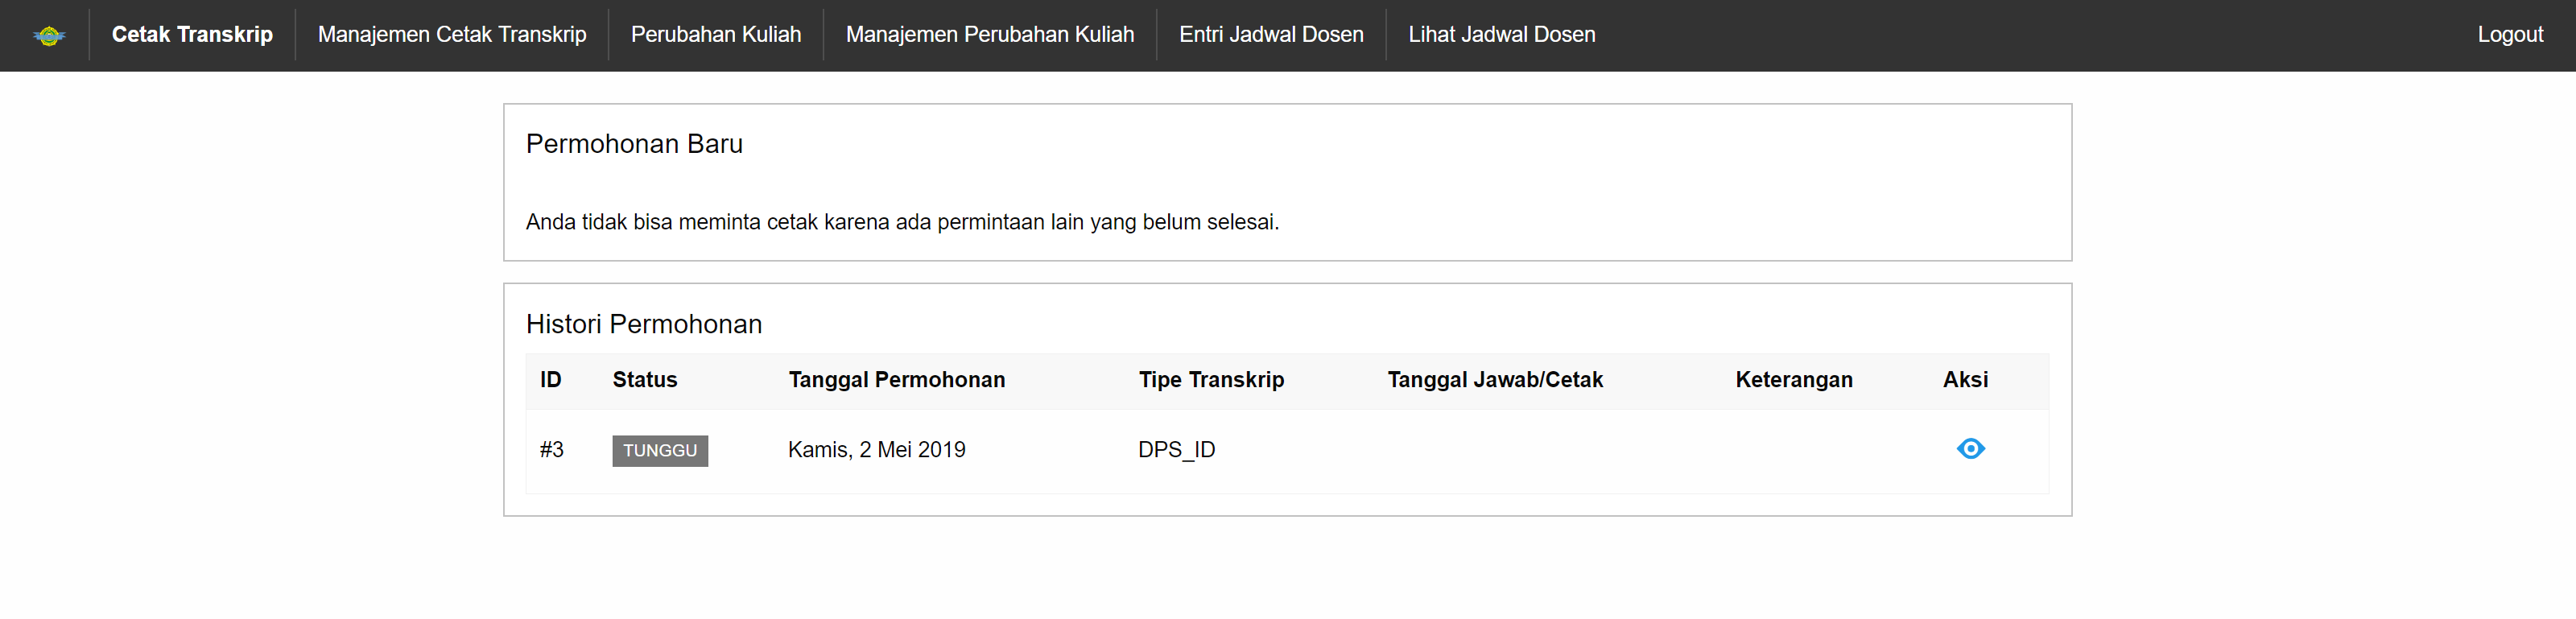
\includegraphics [scale=0.5] {Tampilan-Cetak-Transkrip.PNG}
		\caption{Tampilan Cetak Transkrip}
	\end{figure}
	
	\begin{figure}[h]
		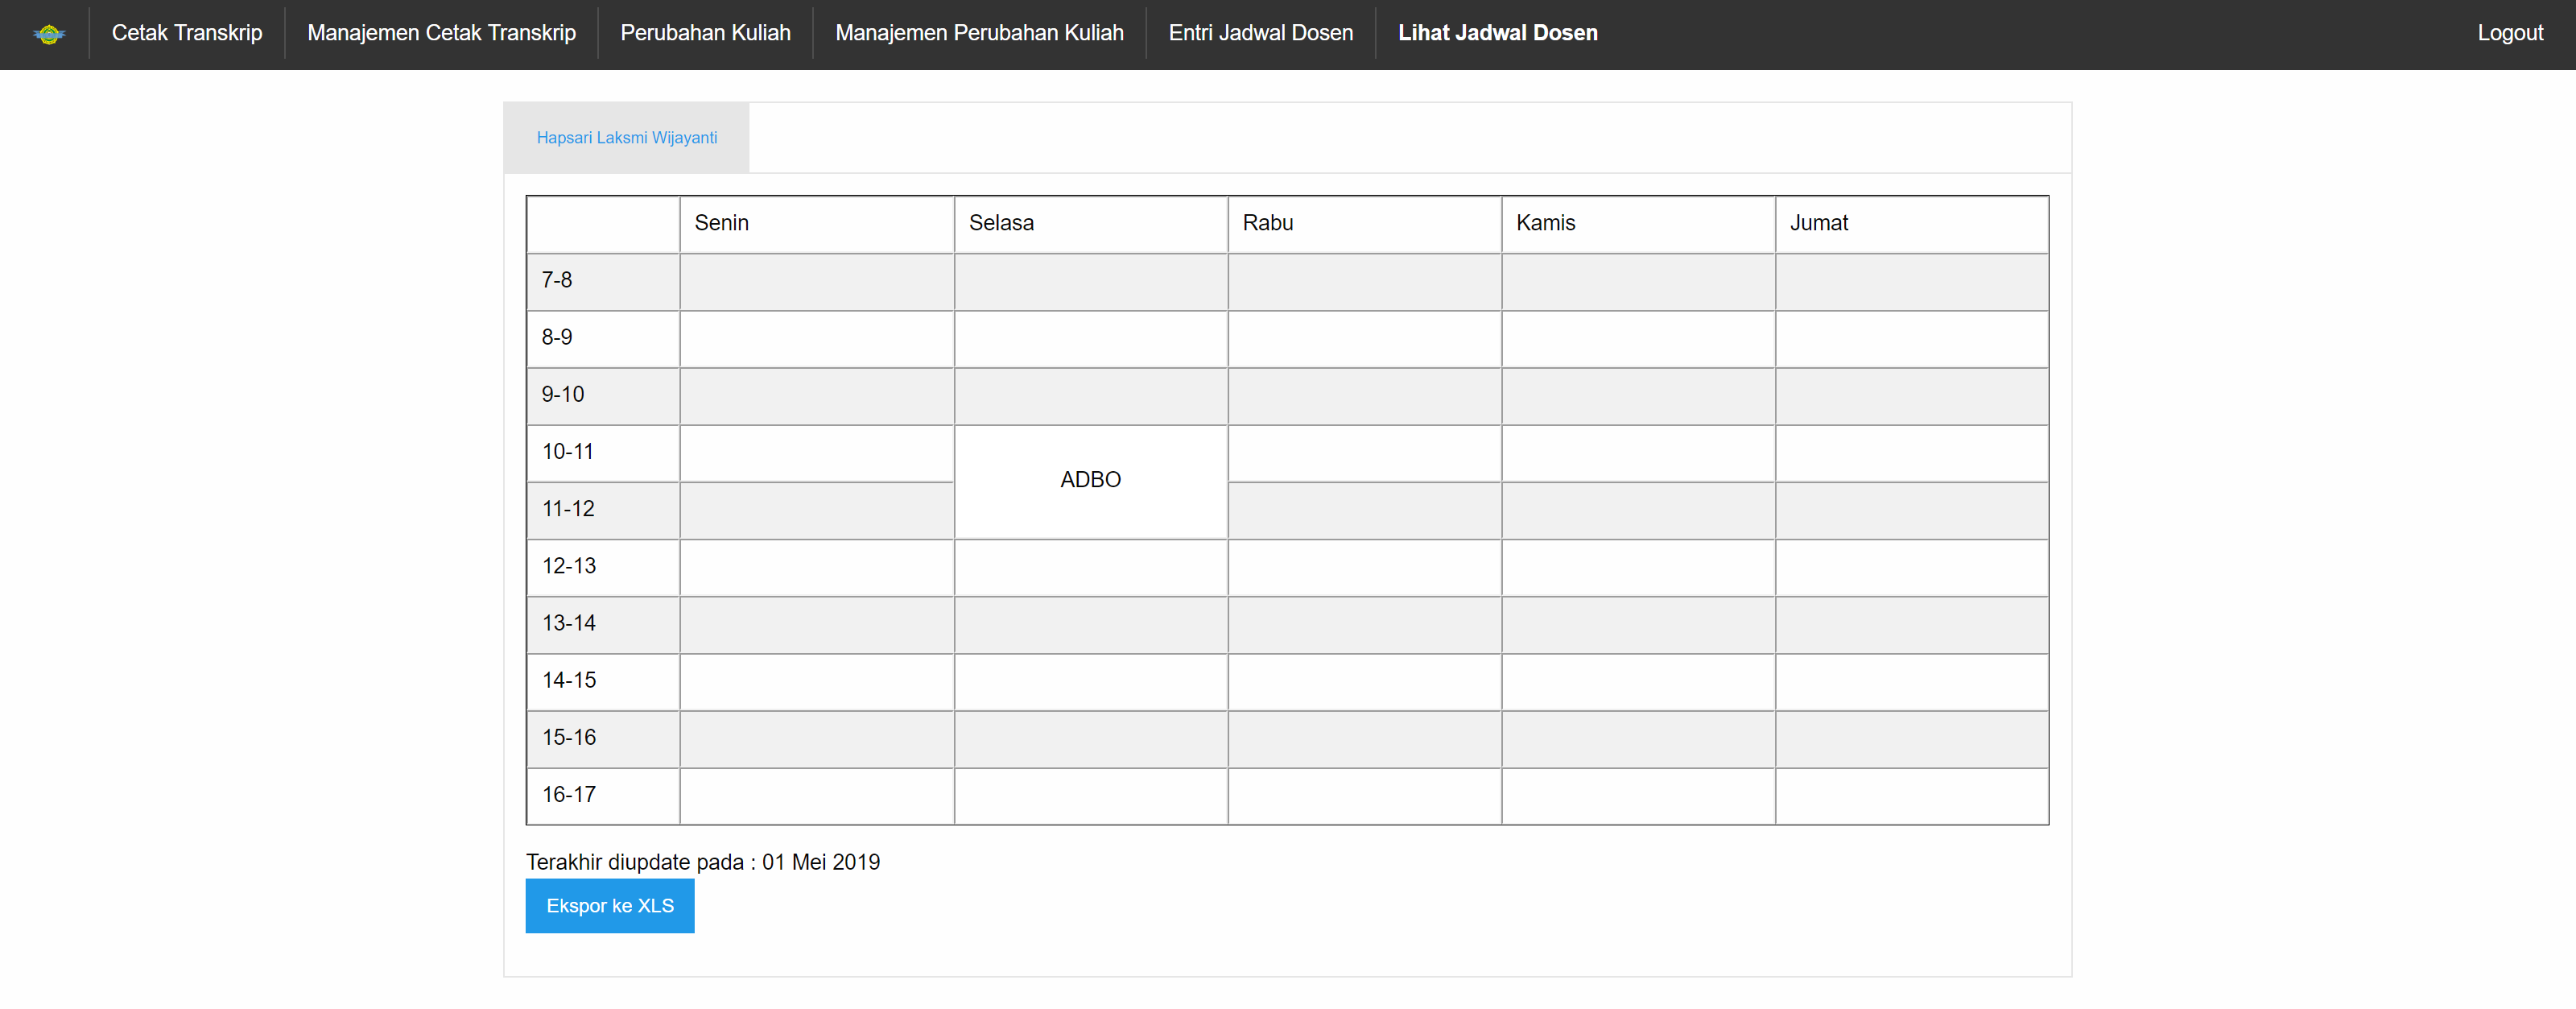
\includegraphics [scale=0.5] {Tampilan-Lihat-Jadwal-Dosen.PNG}
		\caption{Tampilan Lihat Jadwal Dosen}
	\end{figure}
	
	\begin{figure}[h]
		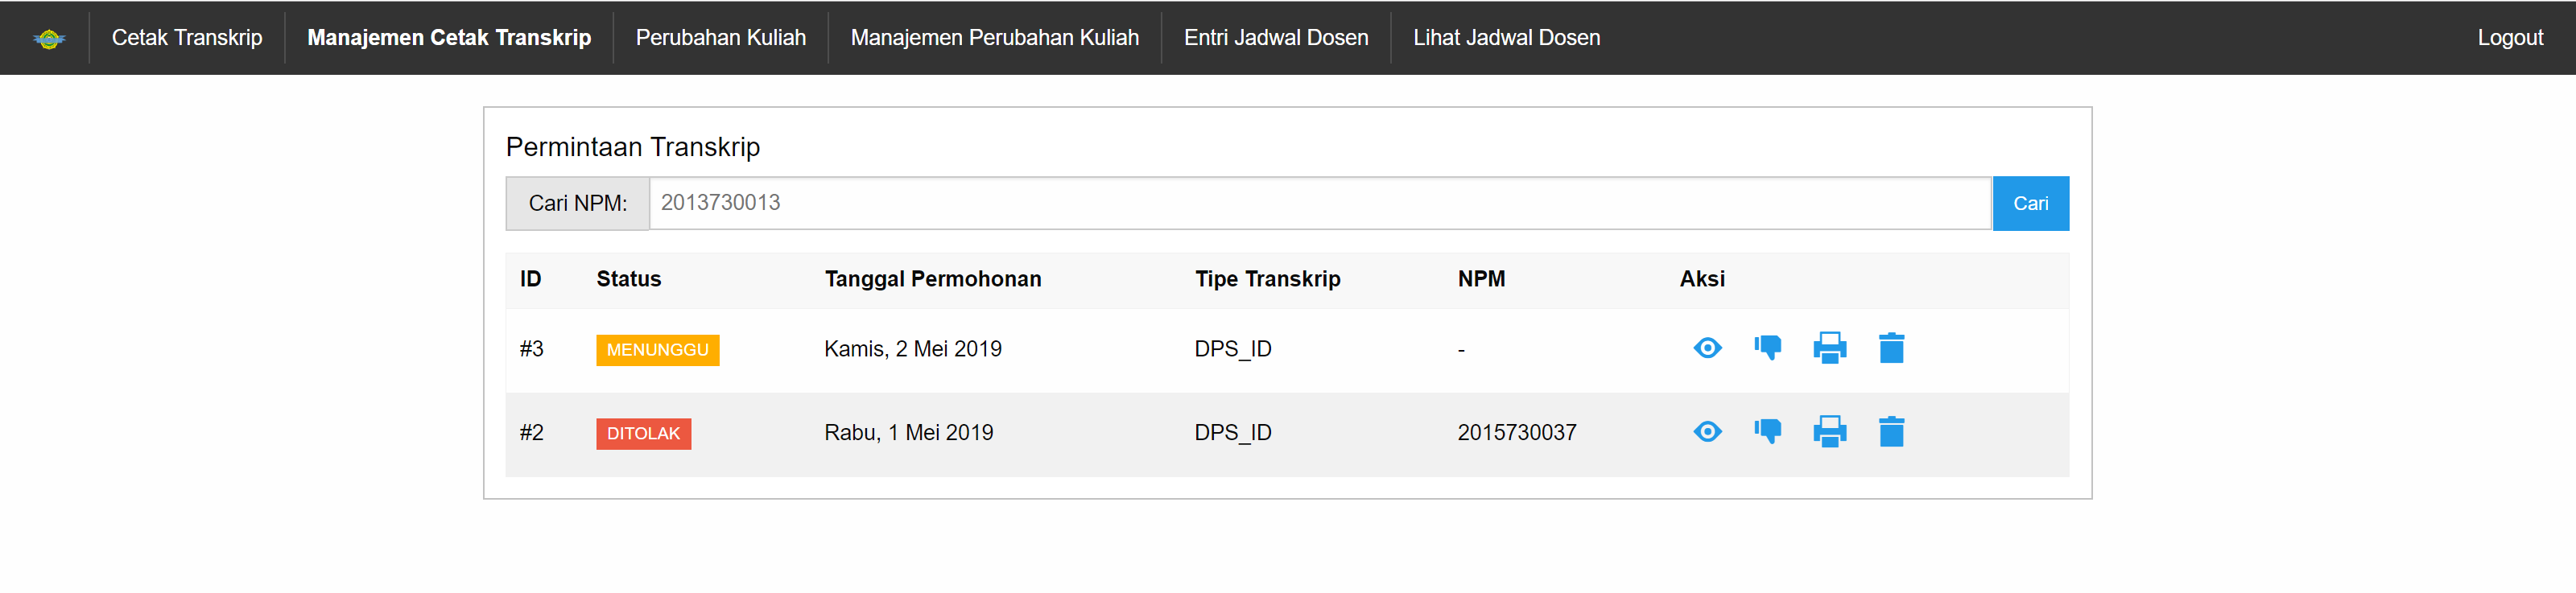
\includegraphics [scale=0.5] {Tampilan-Manajemen-Cetak-Transkrip.PNG}
		\caption{Tampilan-Manajemen-Cetak-Transkrip}
	\end{figure}
	
	\begin{figure}[h]
		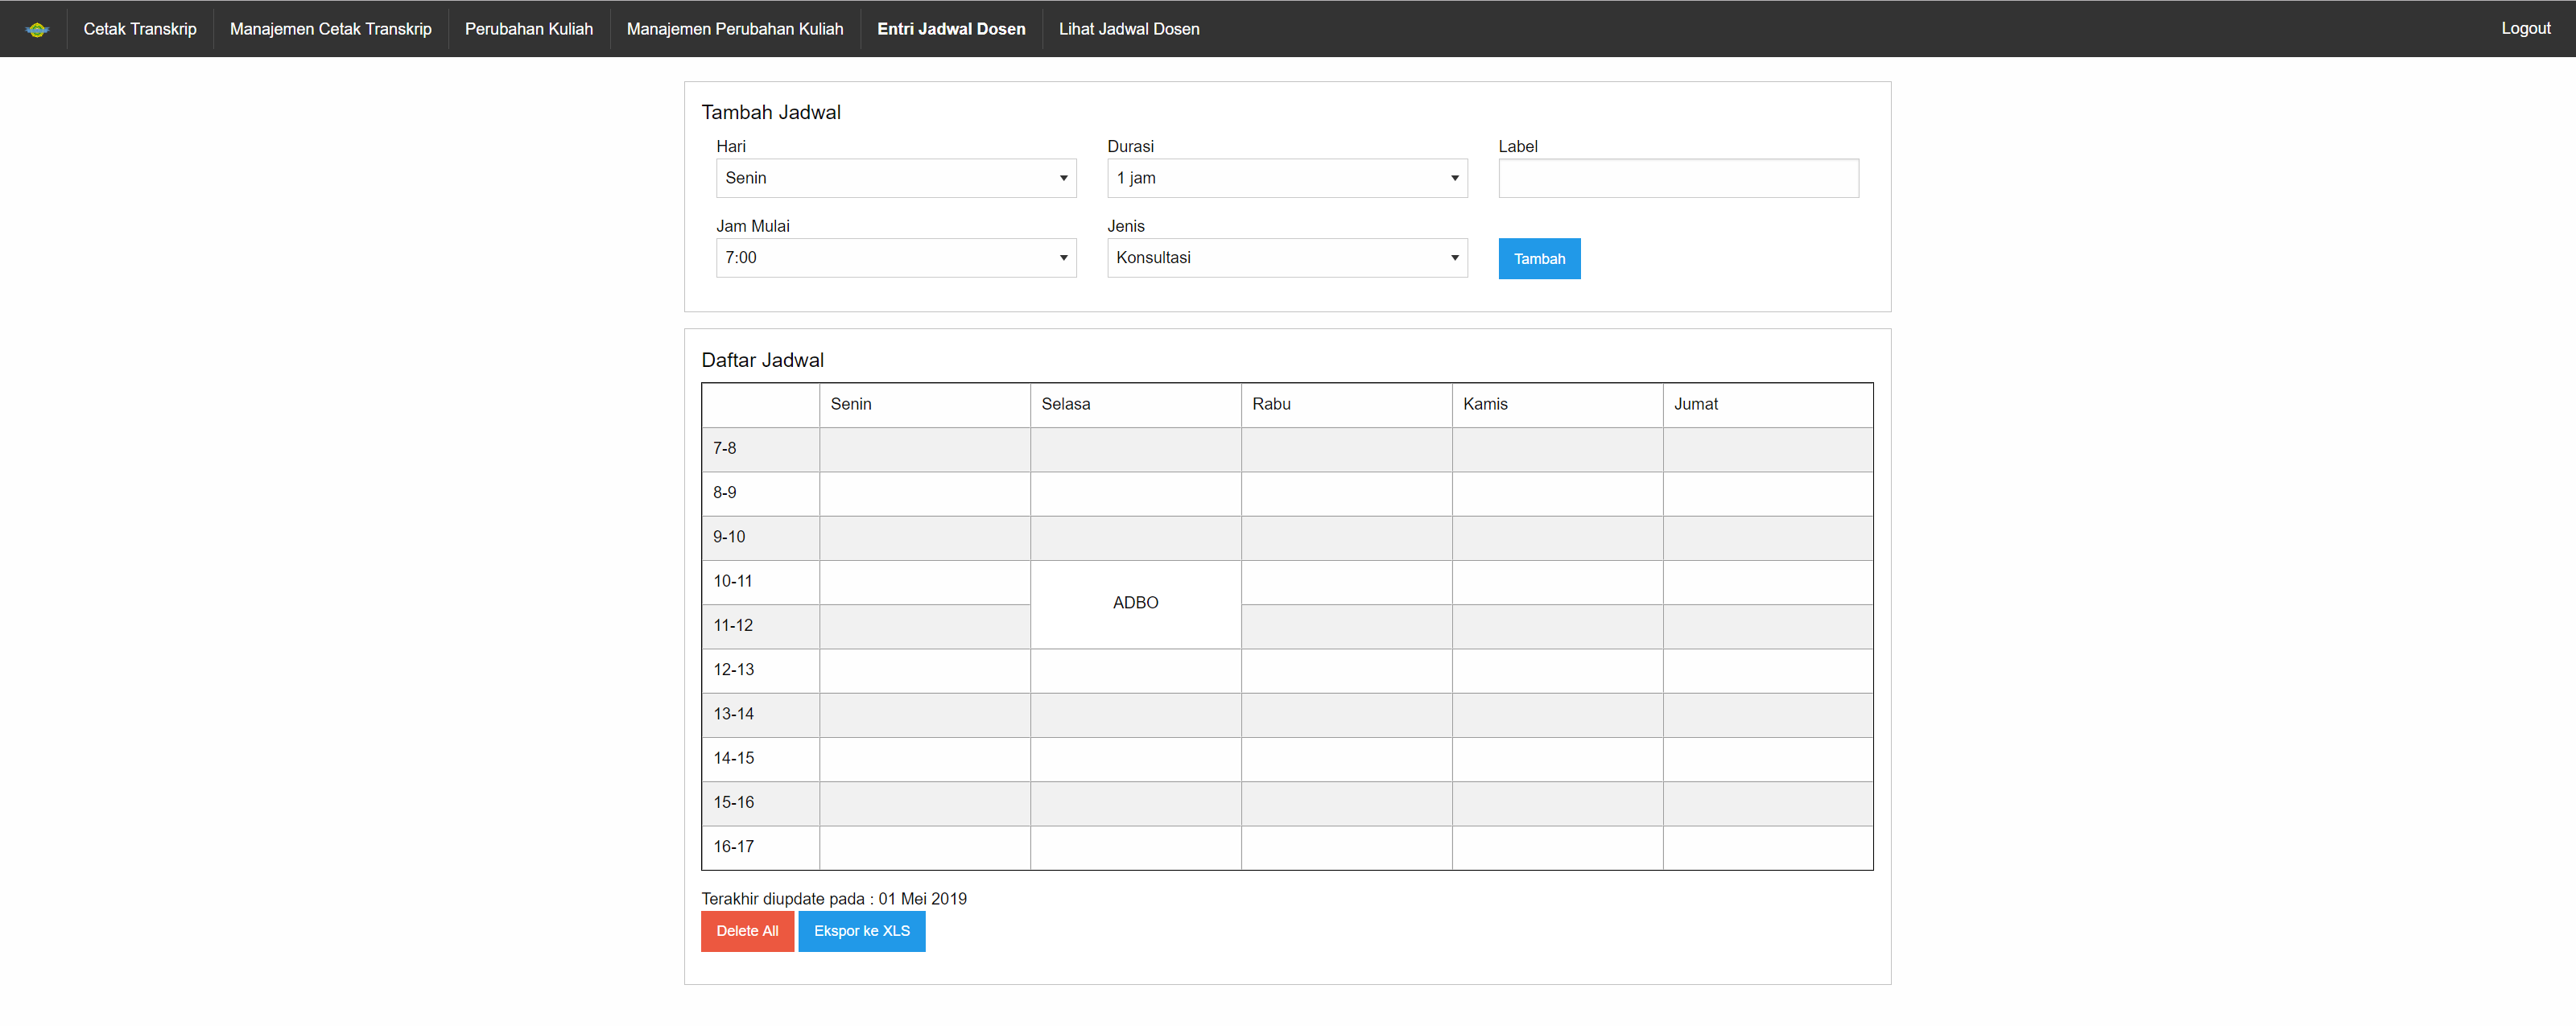
\includegraphics [scale=0.5] {Tampilan-Entri-Jadwal-Dosen.PNG}
		\caption{Tampilan Entri Jadwal Dosen}
	\end{figure}
	
	\begin{figure}[ht!]
		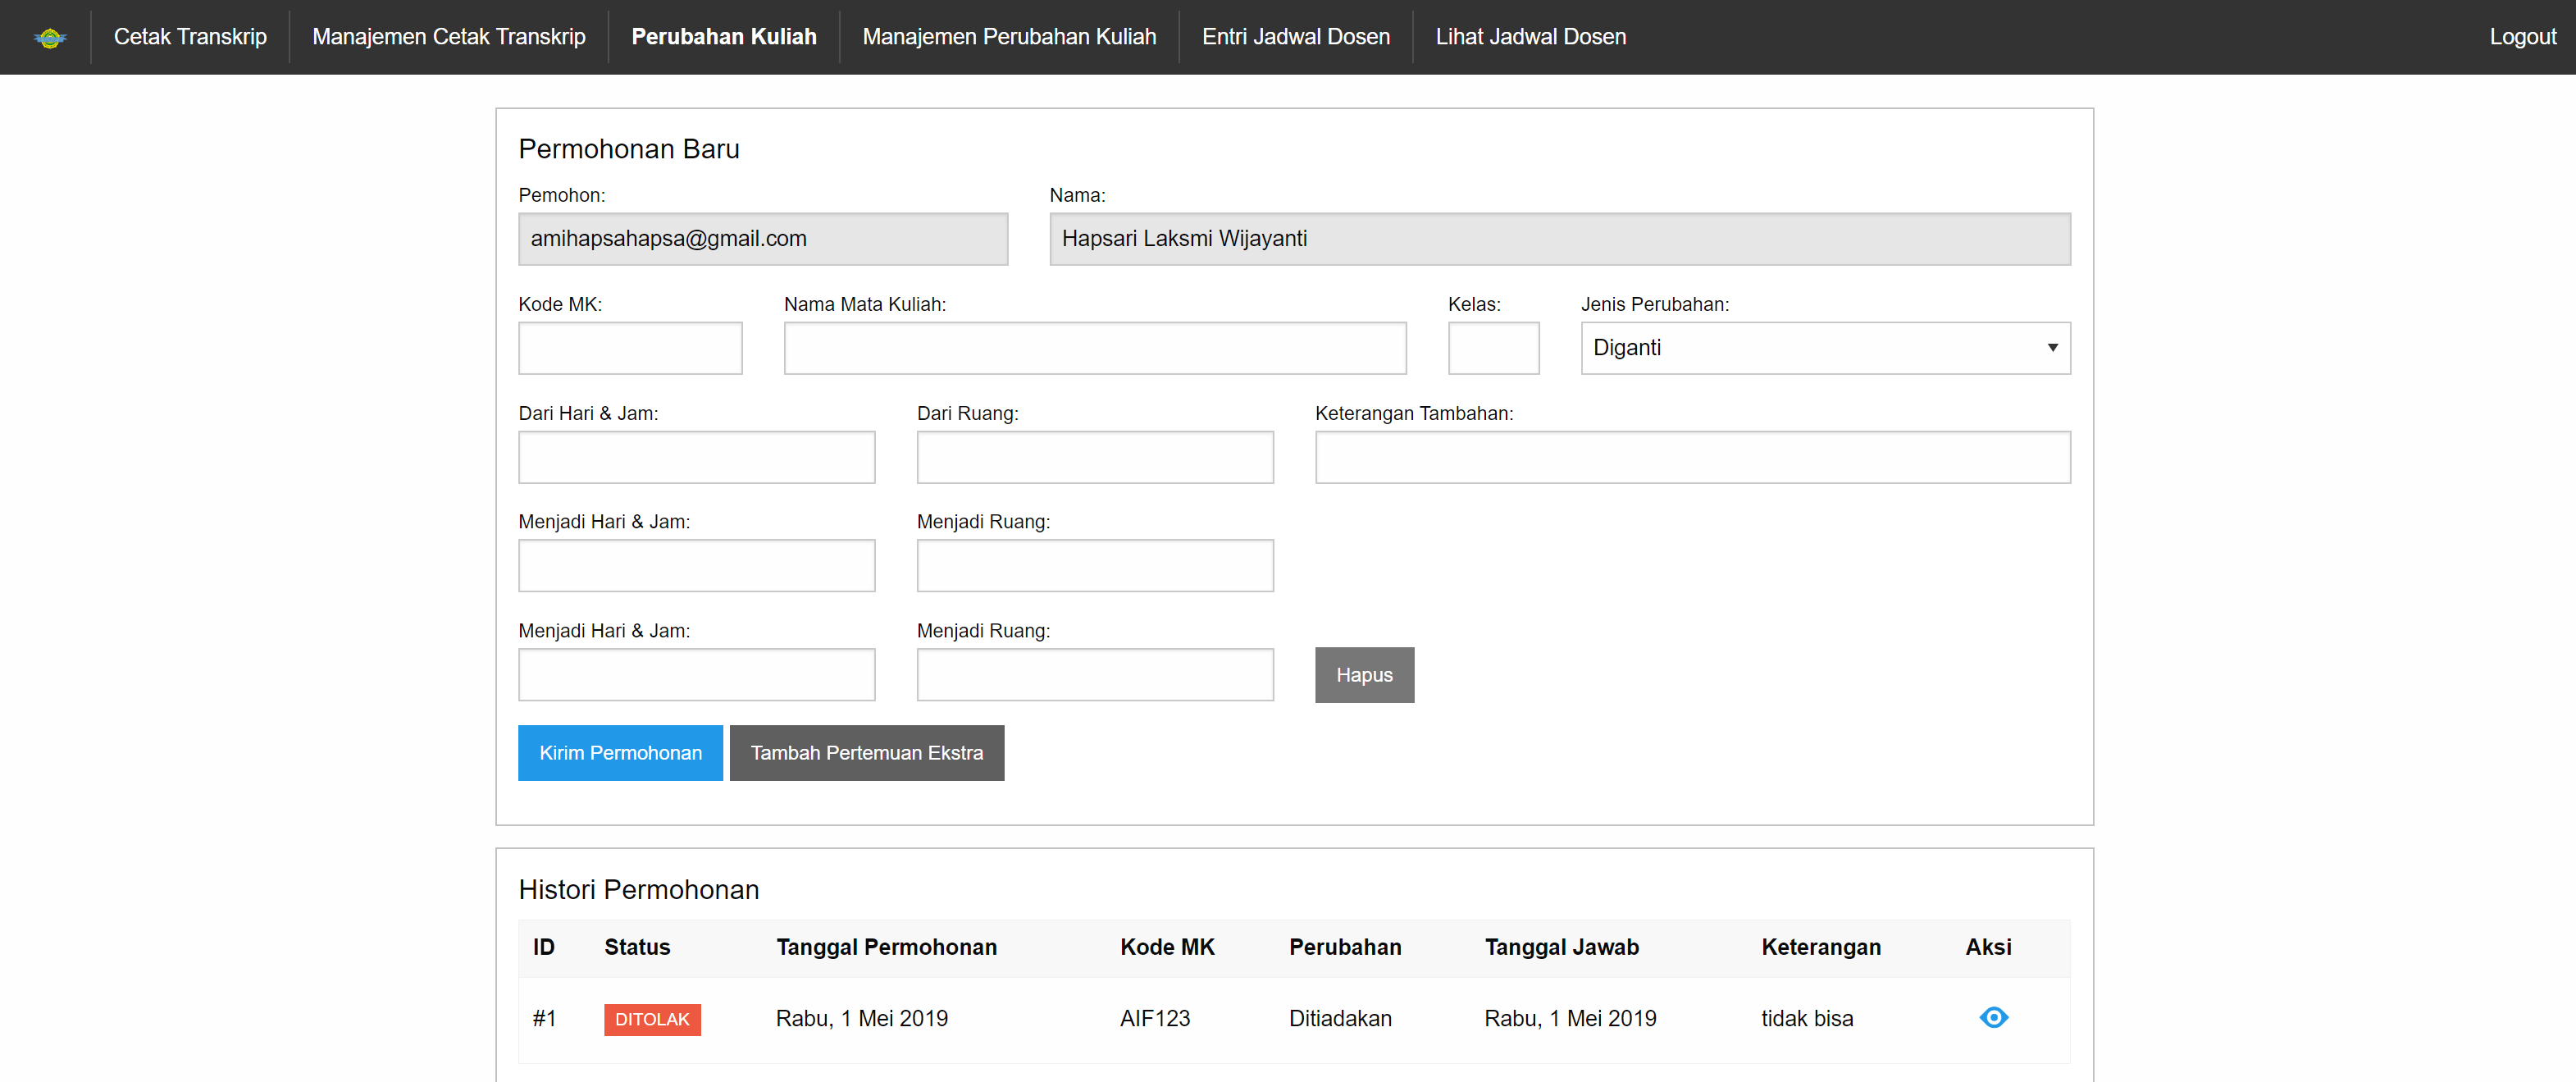
\includegraphics [scale=0.5] {Tampilan-Perubahan-Kuliah.PNG}
		\caption{Tampilan Perubahan Kuliah}
	\end{figure}
	
	\begin{figure}[ht!]
		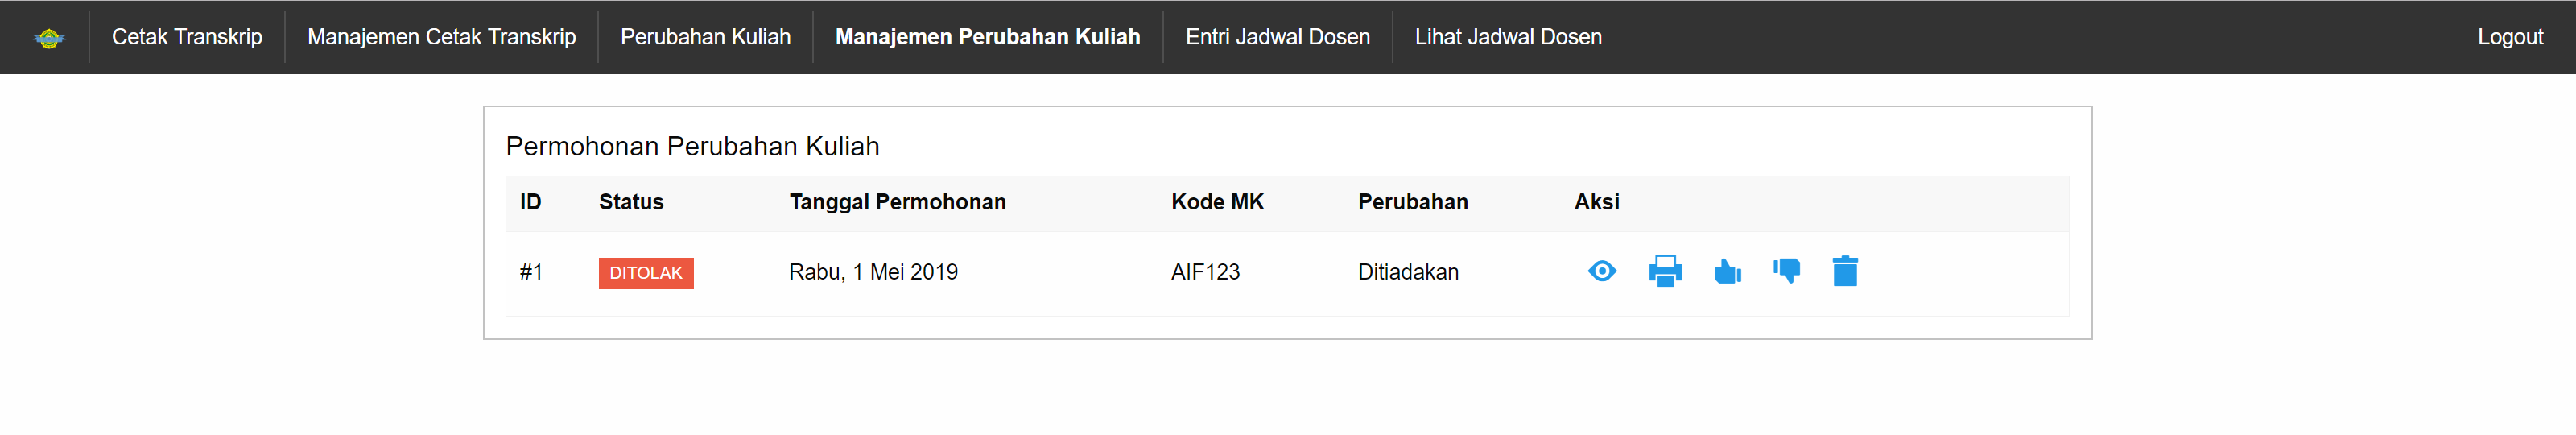
\includegraphics [scale=0.5] {Tampilan-Manajemen-Perubahan-Kuliah.PNG}
		\caption{Tampilan Manajemen Perubahan Kuliah}
	\end{figure}
	
	
	
	
	Meskipun \textit{open-source}, saat ini \textit{Zurb Foundation} tidak sepopuler \textit{framework} \textit{Bootstrap}. 
	\textit{Bootstrap} adalah \textit{ Javascript framework} yang didesain untuk membantu membangun komponen \textit{user interface} yang terdiri dari \textit{CSS, JavaScript/jQuery}, dan \textit{glyphicons}. Pembangunan \textit{website} yang lebih cepat dan besarnya komunitas yang ada berdampak pada banyaknya pengembang \textit{web} yang memanfaatkan \textit{framework Bootstrap}. Sehingga jumlah proyek yang dihasilkan oleh\textit{ framework Bootstrap} lebih banyak dibanding \textit{Zurb Foundation}. 
	
	\section{Tujuan}
	Tujuan yang ingin dicapai dalam penelitian ini :
	\begin{enumerate}
		\item Membuat template cetak transkrip nilai, template manajemen cetak transkrip, template perubahan kuliah, module manajemen perubahan kuliah, modul entri jadwal dosen dan module lihat jadwal dosen dengan framework Bootstrap 4 yang responsive untuk berbagai platform.
		\item Mengimplentasikan plugin yang tersedia dalam library Bootstrap 4.	
	\end{enumerate}
	
	\section{Rumusan Masalah}
	\begin{enumerate}
		\item Bagaimana membuat template manajemen cetak transkrip, manajemen perubahan kuliah dan manajemen jadwal dosen.
		\item Bagaimana mengimplentasikan plugin yang tersedia di dalam Bootstrap 4.	
	\end{enumerate}
	
	\section{Detail Perkembangan Pengerjaan Skripsi}
	Detail bagian pekerjaan skripsi sesuai dengan rencan kerja/laporan perkembangan terkahir :
	\begin{enumerate}
		\item \textbf{Mempelajari framework PHP Codeigniter.}\\
		{\bf Status :} Ada sejak rencana kerja skripsi.\\
		{\bf Hasil :} Mempelajari konsep codeigniter dan mencoba langsung didalam proyek BlueTape \par
		\myparagraph{Application Flow Chart} \par
		Gambar berikut mengilustrasikan bagaimana alur data pada sistem :
		
		\begin{figure} [H]
			\centering  
			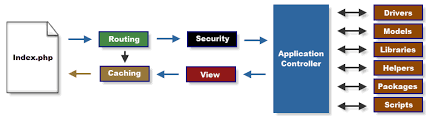
\includegraphics[scale=1.0]{appflowchart.png}  
			\caption{Flow Chart Aplikasi CodeIgniter}
			\label{fig:flow-chart-CodeIgniter} 
		\end{figure}
		
		\begin{enumerate}
			\item \texttt{Index.php} : bertindak sebagai \textit{front controller}, menginisiasi \textit{base resources} yang dibutuhkan untuk menjalankan CodeIgniter.
			\item \texttt{Router} : akan memeriksa permintaan HTTP untuk menetapkan hal apa yang harus dilakukan dengan permintaan tersebut.
			\item \texttt{Cache} : Apabila terdapat \textit{cache}, maka \textit{cache} tersebut akan dikirimkan langsung ke browser, dengan melewati sistem eksekusi normal.
			\item \texttt{Security} : Sebelum \textit{controller} dimuat, \textit{HTTP request} dan \textit{user} mana pun yang mengirimkan data diseleksi dahulu untuk keamanan.
			\item \texttt{Controller} : Terdiri dari \textit{model, core libraries, helpers}, dan \textit{resources} yang dibutuhkan untuk proses \textit{request} tertentu.
			\item \texttt{View} : Tampilan yang telah selesai dirender kemudian dikirim ke \textit{web browser} untuk dilihat. Jika \textit{caching} diaktifkan, tampilan di \textit{cache} terlebih dahulu sehingga pada permintaan selanjutnya dapat dilayani.\cite{codeigniter}
		\end{enumerate}
		
		\myparagraph{CodeIgniter URLs}
		\label{subs:urls}
		Codeigniter menggunakan pendekatan berbasis segment :
		\begin{lstlisting}[frame=single] 
		example.com/class/function/ID
		\end{lstlisting}
		
		\begin{enumerate}
			\item Segmen pertama menyatakan kelas \textit{controller} yang harus dipanggil.
			\item Segmen kedua menyatakan fungsi kelas, atau metode, yang harus dipanggil.
			\item Segmen ketiga dan setiap segmen setelahnya menyatakan ID dan variabel apa pun yang akan diteruskan ke controller.
		\end{enumerate}
		
		\myparagraph{Model}
		\label{subs:model}
		\textit{Model} merepresentasikan struktur data. Biasanya kelas \textit {model} akan berisi fungsi yang membantu untuk \textit{retrieve, insert}, dan \textit{update} informasi di database.
		
		\myparagraph{Anatomi Model}
		\label{sssec:model_1}
		Kelas model akan disimpan dalam direktori \textbf{application/models/directory}.Prototipe dasar dari sebuah model kelas :
		
		\begin{lstlisting}[frame=single]  
		<?php
		class Model_name extends CI_Model {
		
		}
		\end{lstlisting}
		
		\begin{lstlisting}[frame=single]  
		application/models/User_model.php
		\end{lstlisting}
		
		\myparagraph{Loading a Model}
		\label{sssec:model_2}
		
		Model akan dimuat dan dipanggil didalam metode \textit{controller}. Untuk memuat sebuah model maka dapat digunakan metode berikut:
		
		\begin{lstlisting}[frame=single] 
		$this->load->model('model_name');
		\end{lstlisting}
		
		\myparagraph{Koneksi ke Database}
		\label{sssec:model_3}
		Apabila model sudah dimuat, model tersebut tidak terhubung secara langsung ke database. Dengan cara secara manual mengatur konektfitas database melalui parameter ketiga:
		
		\begin{lstlisting}[frame=single]
		$config['hostname'] = 'localhost';
		$config['username'] = 'myusername';
		$config['password'] = 'mypassword';
		$config['database'] = 'mydatabase';
		$config['dbdriver'] = 'mysqli';
		$config['dbprefix'] = '';
		$config['pconnect'] = FALSE;
		$config['db_debug'] = TRUE;
		
		$this->load->model('model_name', '', $config);
		\end{lstlisting}{listing only}
		
		\myparagraph{View}
		\label{subs:view}
		\textit{View} adalah informasi yang sedang dilihat oleh \textit{user}. Sebuah \textit{View} normalnya menjadi sebuah halaman web, namun dalam CodeIgniter, sebuah \textit{view} dapat menjadi sebuah \textit{page fragment} seperti \textit{header} atau \textit{footer}. Dapat juga menjadi halaman RSS, atau tipe apapun dari "page".
		
		\textit{Views} tidak pernah dipanggil secara langsung, harus dimuat dalam sebuah \textit{controller}. Dalam \textit{MVC framework}, \textit{controller} bertanggung jawab untuk mengambil \textit{view} tertentu. 
		
		\myparagraph{Membuat sebuah View} \par
		CodeIgniter memuat view dengan memanggil sebuah file php, misalkan \verb|blogview.php|, dan \textit{developer} dapat mengisinya dengan kode HTML sebgaai berikut:
		\begin{lstlisting}[frame=single] 
		<html>
		<head>
		<title>My Blog</title>
		</head>
		<body>
		<h1>Welcome to my Blog!</h1>
		</body>
		</html>
		\end{lstlisting}
		
		File tersebut akan disimpan di direktori \texttt{application/views/}.
		
		\myparagraph{Loading sebuah View} \par
		
		
		View dapat dimuat dengan membuat file \texttt{view} dengan syntax berikut:
		
		\begin{lstlisting}[frame=single] 
		$this->load->view('name');
		\end{lstlisting}
		
		\noindent Dimana \texttt{name} adalah nama dari file view.
		
		\myparagraph{Memuat Beberapa View} \par
		
		CodeIgniter dapat menangani beberapa panggilan dari dalam controller dengan menggunakan syntax : 
		
		\begin{lstlisting}[frame=single] 
		$this->load->view()
		\end{lstlisting}
		
		Apabila ada lebih dari satu panggilan yang terjadi, maka \textit{views} akan dilampirkan secara bersamaan. Berikut ini kode yang digunakan jika \textit{developer} ingin mempunyai \textit{header view}, \texttt{menu view}, \texttt{content view}, dan \texttt{footer view}. 
		
		
		\begin{lstlisting}[frame=single] 
		<?php
		
		class Page extends CI_Controller {
		
		public function index()
		{
		$data['page_title'] = 'Your title';
		$this->load->view('header');
		$this->load->view('menu');
		$this->load->view('content', $data);
		$this->load->view('footer');
		}
		
		}
		\end{lstlisting}
		
		\myparagraph{Menyimpan Views didalam Sub Direktori}
		
		Untuk menyimpan didalam sub direktori maka dapat menyertakan nama direktori yang memuat \texttt{view}.
		\begin{lstlisting}[frame=single] 
		$this->load->view('directory_name/file_name');
		\end{lstlisting}
		
		\myparagraph{Menambahkan data dinamis ke View}
		
		Data yang dikirim dari controller menuju view berbentuk array atau objek, sehingga akan dilampirkan dalam parameter kedua dalam metode loading view.
		Berikut ini pengguanaan dengan array:
		\begin{lstlisting}[frame=single] 
		$data = array(
		'title' => 'My Title',
		'heading' => 'My Heading',
		'message' => 'My Message'
		);
		
		$this->load->view('blogview', $data);
		\end{lstlisting}
		
		\noindent Kemudian, penggunaan dengan objek:
		\begin{lstlisting}[frame=single] 
		$data = new Someclass();
		$this->load->view('blogview', $data);
		\end{lstlisting}
		
		\noindent Sehingga apabila dimasukan ke controller, kode yang ditambahkan adalah:
		\begin{lstlisting}[frame=single] 
		<?php
		class Blog extends CI_Controller {
		
		public function index()
		{
		$data['title'] = "My Real Title";
		$data['heading'] = "My Real Heading";
		
		$this->load->view('blogview', $data);
		}
		}
		\end{lstlisting}
		
		Untuk mengaksesnya dalam file HTML maka \textit{developer} dapat menggunakan syntax php :
		\begin{lstlisting}[frame=single] 
		<html>
		<head>
		<title><?php echo $title;?></title>
		</head>
		<body>
		<h1><?php echo $heading;?></h1>
		</body>
		</html>
		\end{lstlisting}
		
		\myparagraph{Controller} \par
		\textit{Controller} bertindak sebagai penengah antara Model, View dan \textit{resources} lain yang dibutuhkan untuk proses \textit{HTTP requests} dan untuk menghasilkan sebuah halaman web.
		
		Sebuah \textit{controller} secara sederhana merupakan sebuah file yang dinamakan dengan aturan tertentu sehingga dapat dihubungkan dengan sebuah URl.
		Misalnya untuk URl ini:
		\begin{lstlisting}[frame=single] 
		<?php
		example.com/index.php/blog/
		\end{lstlisting}
		
		Dalam contoh diatas, \textit{Codeigniter} berusaha menemukan \textit{controller} bernama Blog.php dan lalu memuatnya. Ketika sebuah nama \textit{controller} sesuai dengan segmen pertama dari sebuah URl, maka URl akan memuatnya.
		
		Kode berikut merupakan contoh dari \textit{controller} sederhana.
		\begin{lstlisting}[frame=single] 
		<?php
		class Blog extends CI_Controller {
		
		public function index()
		{
		echo 'Hello World'
		}
		}
		\end{lstlisting} 
		
		\myparagraph{Method} \par
		Dalam sebuah kelas \textit{controller} akan memiliki beberapa method, lalu untuk memanggil fungsi didalamnya maka \textit{developer} dapat mengisi segmen kedua dari sebuah url dengan sebuah method. Misalnya controller dengan dua method yaitu \texttt{index()} dan \texttt{comments()}.
		\begin{lstlisting}[frame=single] 
		<?php
		class Blog extends CI_Controller {
		
		public function index()
		{
		echo 'Hello World!';
		}
		
		public function comments()
		{
		echo 'Look at this!';
		}
		}
		\end{lstlisting}
		
		\noindent Pemanggilan method index dapat secara otomatis dilakukan apabila segmen kedua kosong. Namun ada cara lain untuk menamplikan pesan "Hello World" yang dapat dilakukan dengan:
		
		\begin{lstlisting}[frame=single] 
		example.com/index.php/blog/index/
		\end{lstlisting}
		
		\noindent Kemudian untuk memuat method \texttt{comment()} dapat dituliskan sebagai berikut:
		\begin{lstlisting}[frame=single] 
		example.com/index.php/blog/comments/
		\end{lstlisting}
		
		\item \textbf{Mempelajari framework front-end Bootstrap 4 beserta plugin-plugin yang tersedia.}\\
		{\bf Status :} Ada sejak rencana kerja skripsi.\\
		{\bf Hasil :} 
		
		\myparagraph{Sistem Grid Bootstrap}
		Sistem grid Bootstrap menggunakan \textit{container}, \textit{rows}, dan \textit{columns} untuk tata letak dan penyelarasan konten. Selain itu sistem ini dibangun dengan \textit{flexbox} dan seluruhnya \textit{responsive}. \cite{bootstrap:19}
		\begin{figure} [H]
			\centering  
			
\includegraphics[scale=0.7]{gridbasic_bootstrap.png}  
			\caption{Grid pada Bootstrap} 
		\end{figure}
		
		\begin{lstlisting}[frame=single] 
		<div class="container">
		<div class="row">
		<div class="col-sm">
		One of three columns
		</div>
		<div class="col-sm">
		One of three columns
		</div>
		<div class="col-sm">
		One of three columns
		</div>
		</div>
		</div>
		\end{lstlisting}
		Dalam contoh diatas akan dibuat tiga kolom yang memiliki lebar yang sama baik dalam \textit{device} \textit{small, medium, large} dan \textit{extra large} menggunakan kelas grid yang sudah ditentukan sebelumnya oleh Bootstrap. Penggunaan \verb|.container| akan membuat kolom berada ditengah halaman.
		
		Secara detil, bootstrap bekerja dengan cara:
		\begin{itemize}
			\item \textit{Container} disediakan agar konten berada ditengah halaman dan mengisi konten tersebut secara horizontal. Penggunaan \verb|.container| untuk menentukan lebar pixel secara responsif atau \verb|.container-fluid| untuk membuat lebar: 100\%  di semua ukuran \textit{viewport} dan perangkat.
			\item Sebuah baris akan membungkus kolom - kolom. Setiap kolom akan memiliki \textit{padding} secara horizontal yang disebut \verb|gutter| untuk mengatur jarak antar kolom.
			\item Penggunaan flexbox akan membuat lebar pada kolom tidak perlu dispesifikasikan. Misalnya empat variabel dari \verb|.com-sm| akan secara otomatis membuat lebar kolom sebesar 25\%.
			\item Kelas kolom menunjukkan jumlah kolom yang ingin digunakan, dengan maksimal 12 kolom per baris. Apabila \textit{developer} menginginkan tiga kolom yang memiliki lebar yang sama maka dapat menggunakan \colorbox{mygray}{\texttt{.col-4}}.
			\item Lebar kolom diatur dalam persentase, sehingga kolom akan memiliki lebar yang berubah-ubah dan ukuran bergantung dengan elemen \textit{parent} nya.
		\end{itemize}
		\myparagraph{Pilihan Grid}
		Bootstrap menggunakan px untuk grid breakpoint dan lebar container. Ini dikarenakan lebar \textit{viewport} ditentukan denga satuan pixels.
		Berikut ini tabel yang menjelaskan penggunaan kelas grid dalam berbagai perangkat :
		\begin{figure} [H]
			\centering  
			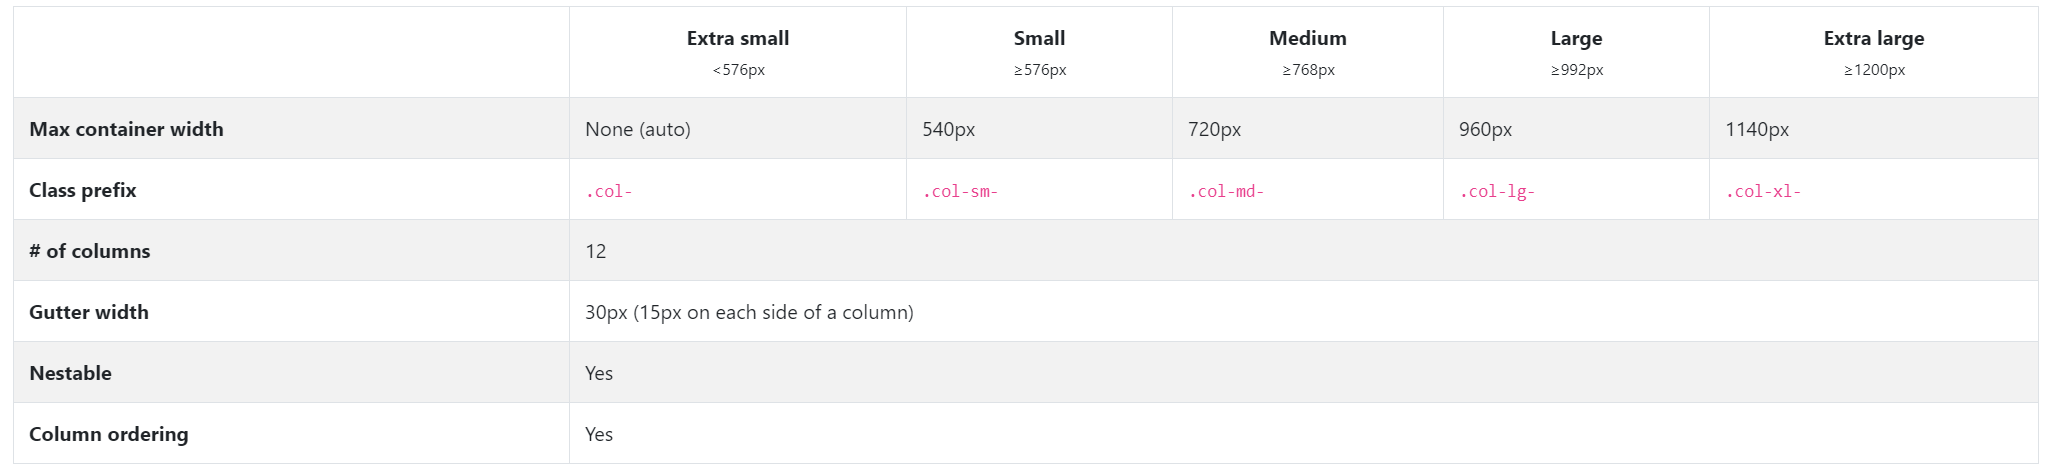
\includegraphics[scale=0.7]{gridoption_bootstrap.png}  
			\caption{Pilihan kelas grid pada Bootstrap} 
		\end{figure}
		
		\myparagraph{Konten}
		\myparagraph{Tabel}
		\paragraph{Tabel Default}
		Dengan penggunaan kelas \verb|.table| pada seluruh tag \colorbox{mygray}{\texttt{<table>}} maka \textit{style} pada bootstrap akan diterapkan, sehingga setiap tabel yang \textit{nested} akan diatur sesuai dengan \textit{parent} nya.
		\begin{figure} [H]
			\centering  
			
\includegraphics[scale=0.7]{tablebasic_bootstrap.png}  
			\caption{Tabel default pada Bootstrap} 
		\end{figure}
		
		\begin{lstlisting}[frame=single] 
		<table class="table">
		<thead>
		<tr>
		<th scope="col">#</th>
		<th scope="col">First</th>
		<th scope="col">Last</th>
		<th scope="col">Handle</th>
		</tr>
		</thead>
		<tbody>
		<tr>
		<th scope="row">1</th>
		<td>Mark</td>
		<td>Otto</td>
		<td>@mdo</td>
		</tr>
		<tr>
		<th scope="row">2</th>
		<td>Jacob</td>
		<td>Thornton</td>
		<td>@fat</td>
		</tr>
		<tr>
		<th scope="row">3</th>
		<td>Larry</td>
		<td>the Bird</td>
		<td>@twitter</td>
		</tr>
		</tbody>
		</table>
		\end{lstlisting}
		
		\myparagraph{Tabel dengan Garis Batas}
		Penggunaan kelas \colorbox{mygray}{\texttt{.table-bordered}} akan membuat tabel memiliki garis batas untuk semua sisi didalam tabel dan \textit{cells}.
		
		\begin{figure} [H]
			\centering  
			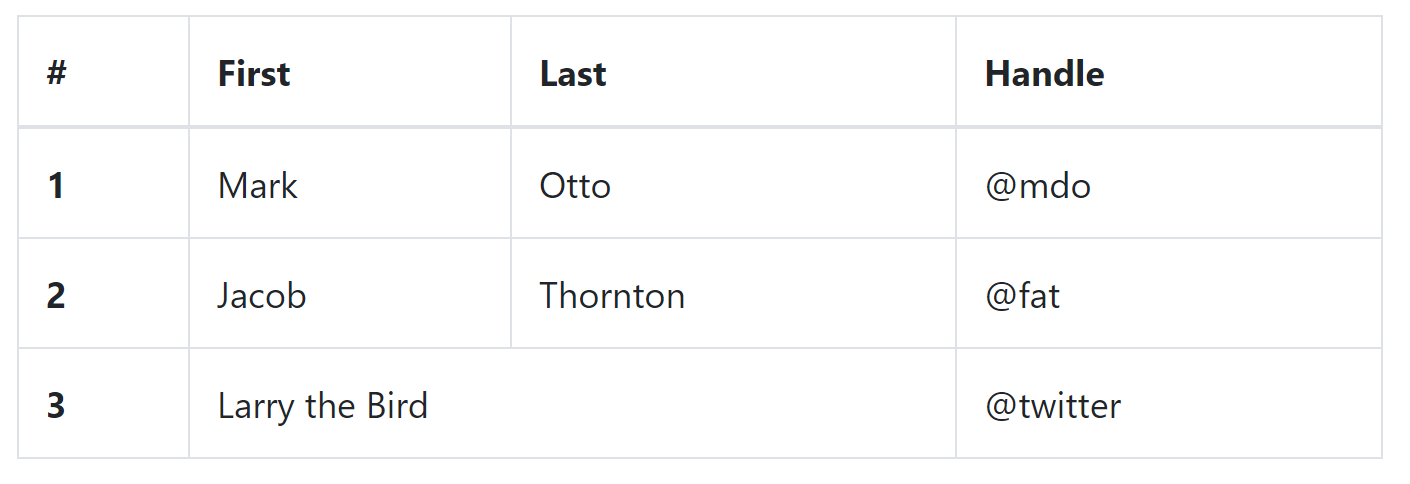
\includegraphics[scale=0.7]{tablebordered_bootstrap.png}  
			\caption{Tabel default pada Bootstrap} 
		\end{figure}
		
		\begin{lstlisting}[frame=single] 
		<table class="table table-bordered">
		<thead>
		<tr>
		<th scope="col">#</th>
		<th scope="col">First</th>
		<th scope="col">Last</th>
		<th scope="col">Handle</th>
		</tr>
		</thead>
		<tbody>
		<tr>
		<th scope="row">1</th>
		<td>Mark</td>
		<td>Otto</td>
		<td>@mdo</td>
		</tr>
		<tr>
		<th scope="row">2</th>
		<td>Jacob</td>
		<td>Thornton</td>
		<td>@fat</td>
		</tr>
		<tr>
		<th scope="row">3</th>
		<td colspan="2">Larry the Bird</td>
		<td>@twitter</td>
		</tr>
		</tbody>
		</table>
		\end{lstlisting}
		
		\myparagraph{Tabel dengan Warna Baris Berbeda}
		Penggunaan kelas \colorbox{mygray}{\texttt{.table-striped}} akan membuat tabel memiliki warna baris berbeda batas antara baris genap dan ganjil didalam tag \colorbox{mygray}{\texttt{<tbody>}}.
		
		\begin{figure} [H]
			\centering  
			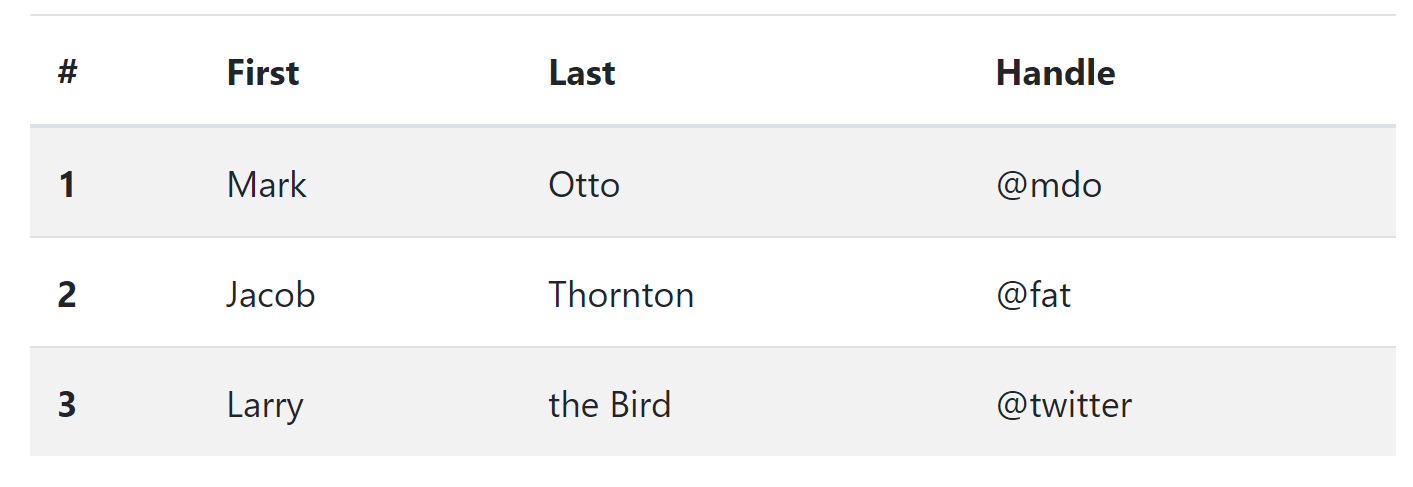
\includegraphics[scale=0.7]{tablestriped_bootstrap.png}  
			\caption{Tabel default pada Bootstrap} 
		\end{figure}
		
		\begin{lstlisting}[frame=single] 
		<table class="table table-striped">
		<thead>
		<tr>
		<th scope="col">#</th>
		<th scope="col">First</th>
		<th scope="col">Last</th>
		<th scope="col">Handle</th>
		</tr>
		</thead>
		<tbody>
		<tr>
		<th scope="row">1</th>
		<td>Mark</td>
		<td>Otto</td>
		<td>@mdo</td>
		</tr>
		<tr>
		<th scope="row">2</th>
		<td>Jacob</td>
		<td>Thornton</td>
		<td>@fat</td>
		</tr>
		<tr>
		<th scope="row">3</th>
		<td colspan="2">Larry the Bird</td>
		<td>@twitter</td>
		</tr>
		</tbody>
		</table>
		\end{lstlisting}
		
		
		\myparagraph{Gambar}
		Gambar dalam Bootstrap akan memiliki sifat \textit{responsive} dengan menerapkan kelas \colorbox{mygray}{\texttt{.img-fluid}} serta mengatur lebar gambar dengan properties \colorbox{mygray}{\texttt{max-width: 100\%}} dan \texttt{height: auto}. Sehingga gambar tidak pernah lebih besar dari \textit{parent} nya. 
		
		\textit{Developer} dapat menyelaraskan (align) sebuah gambar ke kiri atau kanan dengan \textbf{helper float classes} atau \textbf{text alignment classes}. 
		\begin{figure} [H]
			\centering  
			
\includegraphics[scale=0.7]{imgalign_bootstrap.PNG}  
			\caption{\it{Menyelaraskan gambar ke kanan dan kiri pada bootstrap}} 
		\end{figure}
		\begin{lstlisting}[frame=single]
		<img src="..." class="rounded float-left" alt="...">
		<img src="..." class="rounded float-right" alt="...">
		\end{lstlisting}
		
		
		
		\myparagraph{Komponen}
		\myparagraph{Formulir}
		\textit{Form} pada Bootstrap menyediakan beragam tipe input sesuai dengan kebutuhan \textit{user}. Contohnya penggunaan kelas \texttt{email} untuk \textit{input} email atau \texttt{number} untuk input berupa angka.
		\myparagraph{Form Controls}
		\textit{Developer} dapat membuat form menggunakan kelas \colorbox{mygray}{\texttt{.form-control}}. Kelas ini terdiri dari beberapa tag seperti tag\colorbox{mygray}{\texttt{ <input>}}, \colorbox{mygray}{\texttt{<select>}} dan \colorbox{mygray}{\texttt{<textarea>}}.
		\begin{lstlisting}[frame=single, basicstyle=\tiny] 
		<form>
		<div class="form-group">
		<label for="exampleFormControlInput1">Email address</label>
		<input type="email" class="form-control" id="exampleFormControlInput1" placeholder="name@example.com">
		</div>
		<div class="form-group">
		<label for="exampleFormControlSelect1">Example select</label>
		<select class="form-control" id="exampleFormControlSelect1">
		<option>1</option>
		<option>2</option>
		<option>3</option>
		<option>4</option>
		<option>5</option>
		</select>
		</div>
		<div class="form-group">
		<label for="exampleFormControlSelect2">Example multiple select</label>
		<select multiple class="form-control" id="exampleFormControlSelect2">
		<option>1</option>
		<option>2</option>
		<option>3</option>
		<option>4</option>
		<option>5</option>
		</select>
		</div>
		<div class="form-group">
		<label for="exampleFormControlTextarea1">Example textarea</label>
		<textarea class="form-control" id="exampleFormControlTextarea1" rows="3"></textarea>
		</div>
		</form>
		\end{lstlisting}
		
		\begin{figure} [H]
			\centering  
			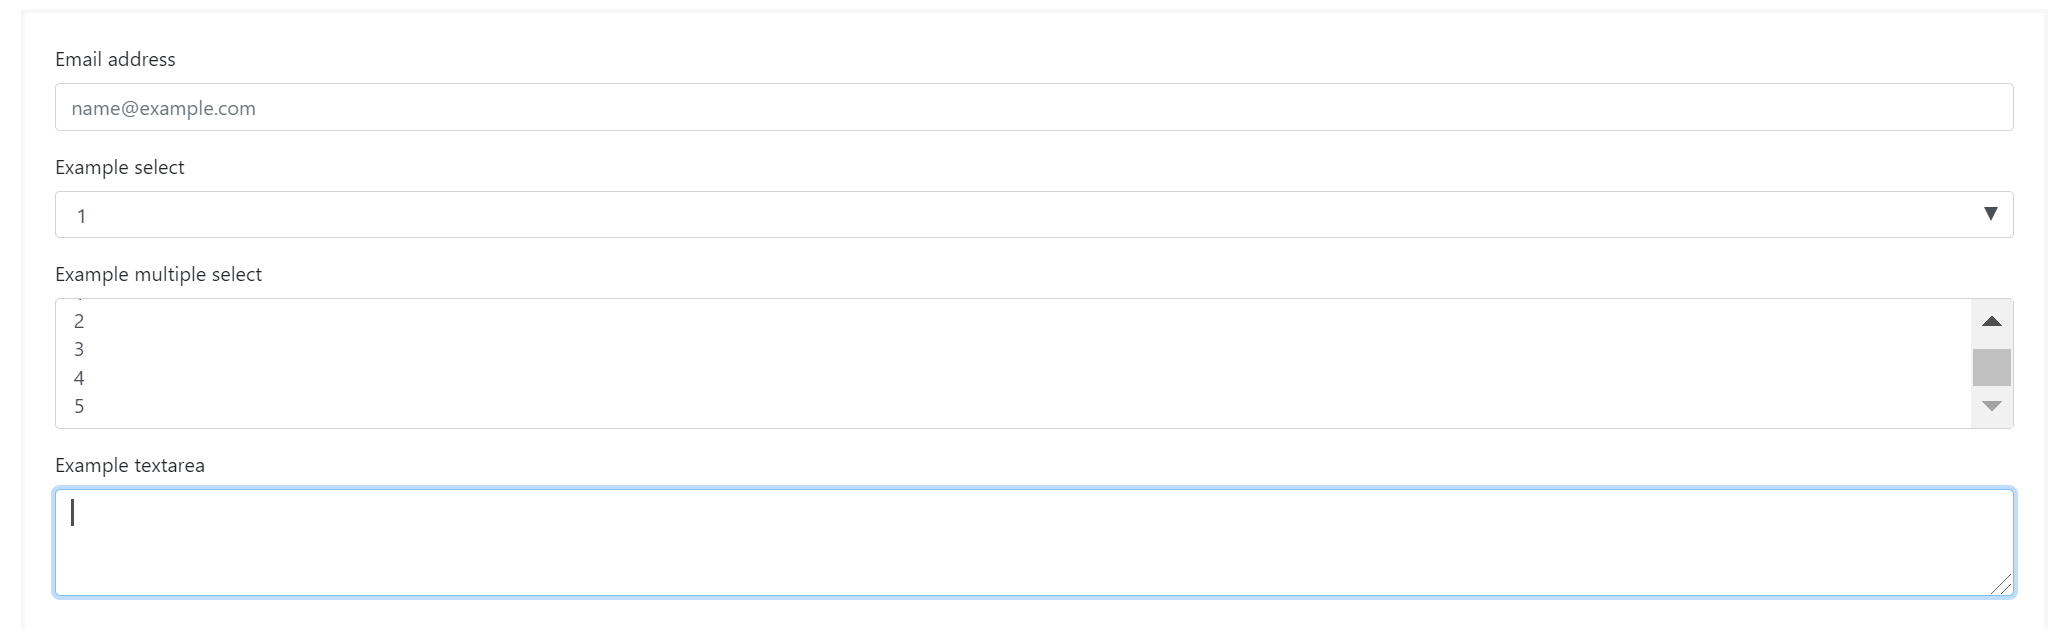
\includegraphics[scale=0.7]{formsbasic_bootstrap.png}  
			\caption{Forms Basic pada Bootstrap} 
		\end{figure} 
		\myparagraph{Column Sizing}
		Bootstrap memungkinkan \textit{developer} untuk menempatkan sejumlah \colorbox{mygray}{\texttt{.col}} di dalam baris \colorbox{mygray}{\texttt{.row}} atau \colorbox{mygray}{\texttt{.form}} dengan lebar tertentu. Misalnya ada tiga buah kolom, kolom pertama memiliki lebar 7 dengan menggunakan kelas \colorbox{mygray}{\texttt{.col-7}} maka dua kolom sisanya akan memiliki lebar yang  memenuhi baris tersebut.
		\begin{figure} [H]
			\centering  
			
\includegraphics[scale=0.7]{columnsizing_bootstrap.png}  
			\caption{Forms Basic pada Bootstrap} 
		\end{figure} 
		\begin{lstlisting}[frame=single] 
		<form>
		<div class="form-row">
		<div class="col-7">
		<input type="text" class="form-control" placeholder="City">
		</div>
		<div class="col">
		<input type="text" class="form-control" placeholder="State">
		</div>
		<div class="col">
		<input type="text" class="form-control" placeholder="Zip">
		</div>
		</div>
		</form>
		\end{lstlisting}
		\myparagraphn{Disabled Forms}
		Penambahan atribut boolean \colorbox{mygray}{\texttt{disabled}} pada sebuah input membuat \textit{user} tidak bisa mengisi data pada \textit{field} tersebut. Untuk non-aktifkan seluruh \textit{field} pada sebuah kolom dapat menambahkan atribut \texttt{disabled} pada tag \colorbox{mygray}{\texttt{<fieldset>}}.
		\begin{figure} [H]
			\centering  
			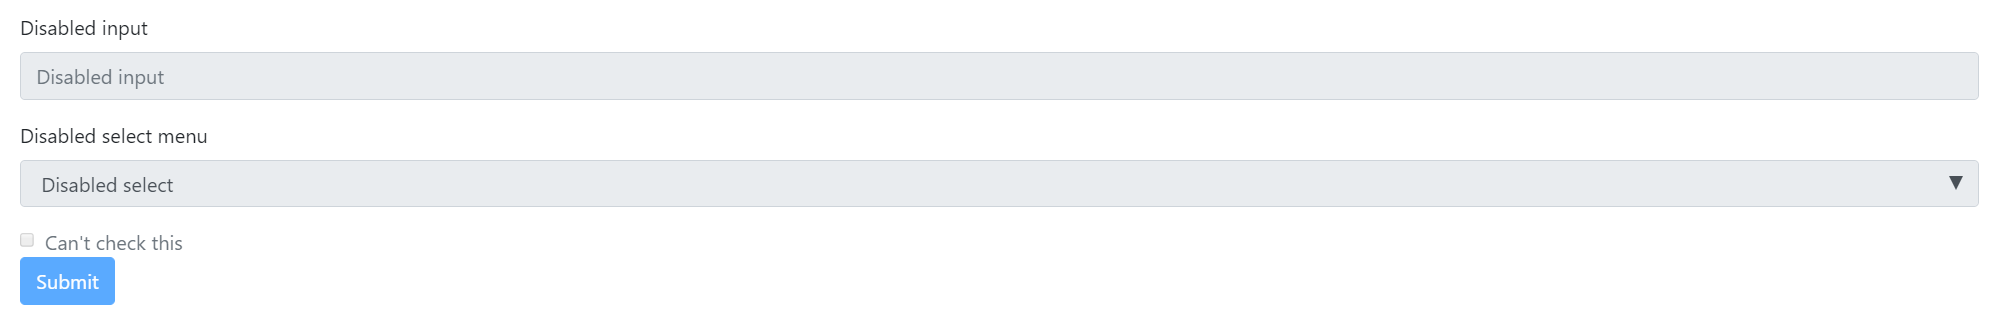
\includegraphics[scale=0.7]{disabledforms_bootstrap.png}  
			\caption{Disabled Basic pada Bootstrap} 
		\end{figure}
		\begin{lstlisting}[frame=single, basicstyle=\tiny] 
		<form>
		<fieldset disabled>
		<div class="form-group">
		<label for="disabledTextInput">Disabled input</label>
		<input type="text" id="disabledTextInput" class="form-control" placeholder="Disabled input">
		</div>
		<div class="form-group">
		<label for="disabledSelect">Disabled select menu</label>
		<select id="disabledSelect" class="form-control">
		<option>Disabled select</option>
		</select>
		</div>
		<div class="form-check">
		<input class="form-check-input" type="checkbox" id="disabledFieldsetCheck" disabled>
		<label class="form-check-label" for="disabledFieldsetCheck">
		Can't check this
		</label>
		</div>
		<button type="submit" class="btn btn-primary">Submit</button>
		</fieldset>
		</form>
		\end{lstlisting}
		\myparagraph{Button}
		Bootstrap memasukan beberapa button dengan \textit{style} yang sudah didefinisikan sebelumnya, membuat setiap button akan memiliki makna nya sendiri.
		\begin{figure} [H]
			\centering  
			
\includegraphics[scale=0.7]{buttons_bootstrap.png}  
			\caption{Button pada Bootstrap} 
		\end{figure}
		\begin{lstlisting}[frame=single] 
		<button type="button" class="btn btn-primary">Primary</button>
		<button type="button" class="btn btn-secondary">Secondary</button>
		<button type="button" class="btn btn-success">Success</button>
		<button type="button" class="btn btn-danger">Danger</button>
		<button type="button" class="btn btn-warning">Warning</button>
		<button type="button" class="btn btn-info">Info</button>
		<button type="button" class="btn btn-light">Light</button>
		<button type="button" class="btn btn-dark">Dark</button>
		
		<button type="button" class="btn btn-link">Link</button>
		\end{lstlisting}
		
		
		\myparagraph{Button with Dropdowns}
		\begin{lstlisting}[frame=single, basicstyle=\tiny]
		<div class="input-group mb-3">
		<div class="input-group-prepend">
		<button class="btn btn-outline-secondary dropdown-toggle" type="button" data-toggle="dropdown"
		aria-haspopup="true" aria-expanded="false">Dropdown</button>
		<div class="dropdown-menu">
		<a class="dropdown-item" href="#">Action</a>
		<a class="dropdown-item" href="#">Another action</a>
		<a class="dropdown-item" href="#">Something else here</a>
		<div role="separator" class="dropdown-divider"></div>
		<a class="dropdown-item" href="#">Separated link</a>
		</div>
		</div>
		<input type="text" class="form-control" aria-label="Text input with dropdown button">
		</div>
		
		<div class="input-group">
		<input type="text" class="form-control" aria-label="Text input with dropdown button">
		<div class="input-group-append">
		<button class="btn btn-outline-secondary dropdown-toggle" type="button" data-toggle="dropdown"
		aria-haspopup="true" aria-expanded="false">Dropdown</button>
		<div class="dropdown-menu">
		<a class="dropdown-item" href="#">Action</a>
		<a class="dropdown-item" href="#">Another action</a>
		<a class="dropdown-item" href="#">Something else here</a>
		<div role="separator" class="dropdown-divider"></div>
		<a class="dropdown-item" href="#">Separated link</a>
		</div>
		</div>
		</div>
		\end{lstlisting}
		
		\begin{figure} [H]
			\centering  
			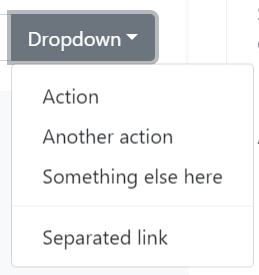
\includegraphics[scale=1.0]{buttonsdropdown_bootstrap.PNG}  
			\caption{Tombol \textit{dropdown} pada Bootstrap} 
		\end{figure}
		
		\myparagraph{Badge}
		Kelas \colorbox{mygray}{\texttt{badge}} dan \colorbox{mygray}{\texttt{.badge-*}} di dalam sebuah \colorbox{mygray}{\texttt{<a>}} akan memberikan badge yang dapat diberi atribut \textit{hover} dan \textit{focus}. 
		\begin{lstlisting}[frame=single, basicstyle=\tiny]
		<a href="#" class="badge badge-primary">Primary</a>
		<a href="#" class="badge badge-secondary">Secondary</a>
		<a href="#" class="badge badge-success">Success</a>
		<a href="#" class="badge badge-danger">Danger</a>
		<a href="#" class="badge badge-warning">Warning</a>
		<a href="#" class="badge badge-info">Info</a>
		<a href="#" class="badge badge-light">Light</a>
		<a href="#" class="badge badge-dark">Dark</a>
		\end{lstlisting}
		
		\begin{figure} [H]
			\centering  
			
\includegraphics[scale=1.0]{badge_bootstrap.PNG}  
			\caption{Badge pada Bootstrap} 
		\end{figure}
		
		\myparagraph{Card}
		Kelas \colorbox{mygray}{\texttt{.card}} adalah kontainer konten yang fleksibel dan bisa diatur lebarnya. Sebuah card memiliki sebuah \textit{headers} dan \textit{footers}.
		
		\begin{lstlisting}[frame=single, basicstyle=\tiny]
		<div class="card">
		<div class="card-header">
		Featured
		</div>
		<div class="card-body">
		<h5 class="card-title">Special title treatment</h5>
		<p class="card-text">With supporting text below as 
		a natural lead-in to additional content.</p>
		<a href="#" class="btn btn-primary"card>Go somewhere</a>
		</div>
		</div>
		\end{lstlisting}
		
		\begin{figure} [H]
			\centering  
			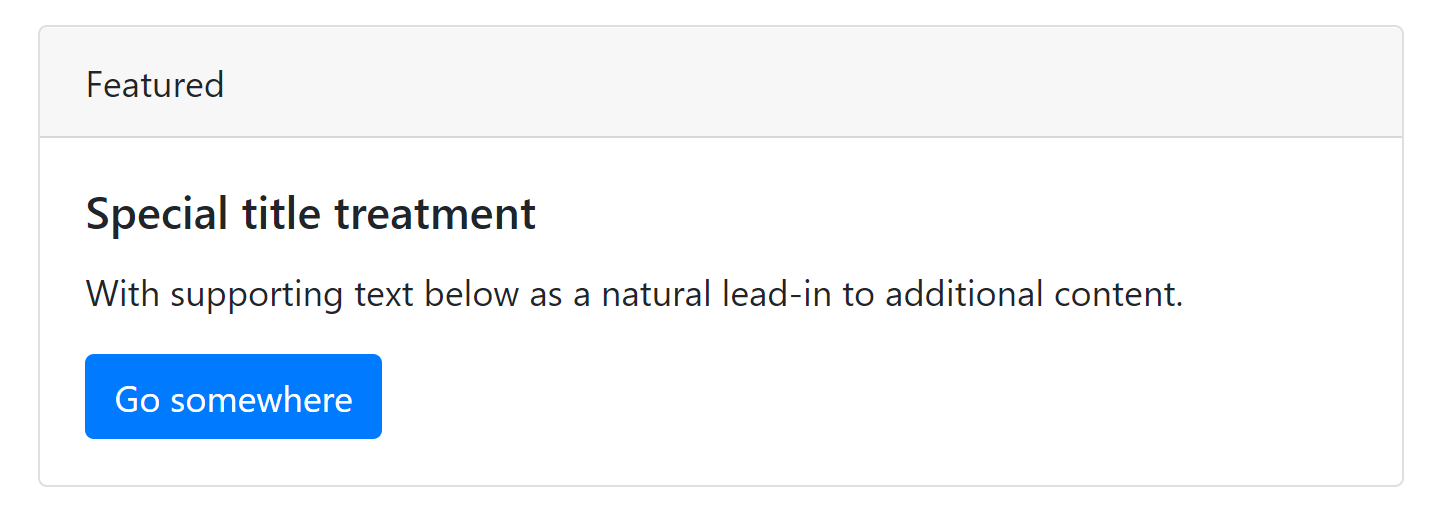
\includegraphics[scale=1.0]{card_bootstrap.PNG}  
			\caption{Card pada Bootstrap} 
		\end{figure}
		
		\myparagraph{Navigation Bar}
		Navbar pada Bootstrap terdiri dari beberapa sub-komponen yang bisa digunakan sesuai dengan kebutuhan:
		\begin{itemize}
			\item \colorbox{mygray}{\texttt{.navbar-brand}} : Komponen untuk menampilkan nama perusahaan, nama produk atau nama proyek.
			\item \colorbox{mygray}{\texttt{.navbar-nav}} : Komponen untuk membuat navigasi memiliki lebar yang memenuhi layar.
			\item \colorbox{mygray}{\texttt{.navbar-toggler}} : Komponen yang digunakan bersamaan dengan plugin untuk membuat efek jatuh dan perilaku navigasi lainnya.
			\item \colorbox{mygray}{\texttt{.form-inline}} : Komponen untuk pengaturan formulir dan aksi.
			\item \colorbox{mygray}{\texttt{.collapse.navbar-collapse}} : Komponen untuk mengelompokkan dan menyembunyikan \textit{navigation bar} dengan sebuah breakpoint induknya.
			%breakpoint : titik dimana terjadi perubahan (xs(br:0px), sm.. )
		\end{itemize}
		Berikut ini merupakan semua sub-komponen yang termasuk dalam navigation bar, navbar mengimplementasikan tema \colorbox{mygray}{\texttt{light-themed}} yang secara otomatis menyembunyilan menu pada breakpoint \texttt{lg}
		\begin{figure} [H]
			\centering  
			
\includegraphics[scale=1.0]{navbar_bootstrap.PNG}  
			\caption{Navigation Bar pada Bootstrap} 
		\end{figure}
		
		\begin{lstlisting}[frame=single, basicstyle=\tiny] 
		<nav class="navbar navbar-expand-lg navbar-light bg-light">
		<a class="navbar-brand" href="#">Navbar</a>
		<button class="navbar-toggler" type="button" data-toggle="collapse" data-target="#navbarSupportedContent" 
		aria-controls="navbarSupportedContent" aria-expanded="false" aria-label="Toggle navigation">
		<span class="navbar-toggler-icon"></span>
		</button>
		
		<div class="collapse navbar-collapse" id="navbarSupportedContent">
		<ul class="navbar-nav mr-auto">
		<li class="nav-item active">
		<a class="nav-link" href="#">Home <span class="sr-only">(current)</span></a>
		</li>
		<li class="nav-item">
		<a class="nav-link" href="#">Link</a>
		</li>
		<li class="nav-item dropdown">
		<a class="nav-link dropdown-toggle" href="#" id="navbarDropdown" role="button" 
		data-toggle="dropdown" aria-haspopup="true" aria-expanded="false">
		Dropdown
		</a>
		<div class="dropdown-menu" aria-labelledby="navbarDropdown">
		<a class="dropdown-item" href="#">Action</a>
		<a class="dropdown-item" href="#">Another action</a>
		<div class="dropdown-divider"></div>
		<a class="dropdown-item" href="#">Something else here</a>
		</div>
		</li>
		<li class="nav-item">
		<a class="nav-link disabled" href="#">Disabled</a>
		</li>
		</ul>
		<form class="form-inline my-2 my-lg-0">
		<input class="form-control mr-sm-2" type="search" placeholder="Search" aria-label="Search">
		<button class="btn btn-outline-success my-2 my-sm-0" type="submit">Search</button>
		</form>
		</div>
		</nav>
		\end{lstlisting}
		
		\myparagraph{Modal}
		Bagaimana Modal bekerja :
		\begin{itemize}
			\item Modal dibangun dengan HTML, CSS dan Javascript. 
			\item Menekan modal "backdrop" otomatis menutup komponen modal.
			\item Bootstrap hanya mendukung satu modal dalam sebuah window pada satu waktu. Penggunaan modal yang bercabang dalam Bootstrap dipercaya memberikan \textit{user experience} yang buruk.
			\item Modal menggunakann \texttt{position: fixed} yang diletakkan pada posisi teratas dalam kode agar terhindar dari \textit{bug} yang disebabkan elemen lain yang memiliki posisi \textit{fixed}. 
		\end{itemize}
		Komponen modal terdiri dari modal headerm modal body dan modal footer (opsional).
		\begin{figure} [H]
			\centering  
			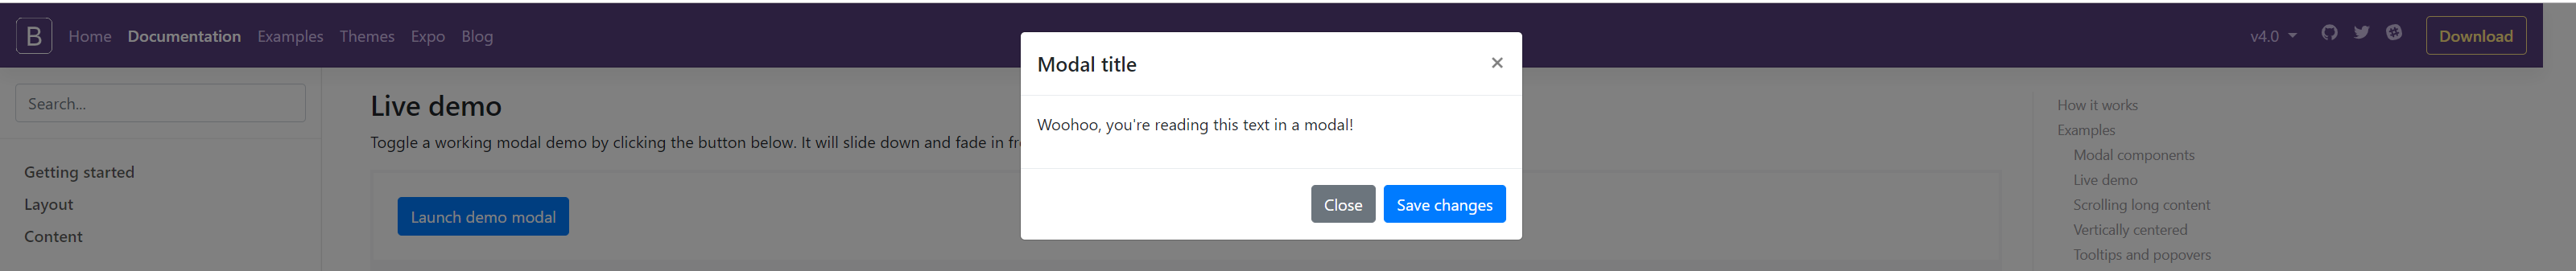
\includegraphics[scale=0.5]{livemodal_bootstrap.png}  
			\caption{Modal pada Bootstrap} 
		\end{figure}
		\begin{lstlisting}[frame=single, basicstyle=\tiny] 
		<!-- Button trigger modal -->
		<button type="button" class="btn btn-primary" data-toggle="modal" data-target="#myModal">
		Launch demo modal
		</button>
		
		<!-- Modal -->
		<div class="modal fade" id="exampleModal" tabindex="-1" role="dialog" 
		aria-labelledby="exampleModalLabel" aria-hidden="true">
		<div class="modal-dialog" role="document">
		<div class="modal-content">
		<div class="modal-header">
		<h5 class="modal-title" id="exampleModalLabel">Modal title</h5>
		<button type="button" class="close" data-dismiss="modal" aria-label="Close">
		<span aria-hidden="true">&times;</span>
		</button>
		</div>
		<div class="modal-body">
		...
		</div>
		<div class="modal-footer">
		<button type="button" class="btn btn-secondary" data-dismiss="modal">Close</button>
		<button type="button" class="btn btn-primary">Save changes</button>
		</div>
		</div>
		</div>
		</div>
		\end{lstlisting}
		
		\myparagraph{Ikon}
		Bootstrap tidak memiliki \textit{library} ikon secara \textit{default}, sehingga ikon yang digunakan diambil dari \textbf{Font Awesome}. Penggunaan ikon dengan menggunakan tag \colorbox{mygray}{\texttt{<i>}} yang disertai dengan kelas \colorbox{mygray}{\texttt{fa}} (font-awesome). 
		
		\begin{lstlisting}[frame=single]
		<i class="fa fa-coffee"></i>
		\end{lstlisting}
		
		\begin{figure} [H]
			\centering  
			
\includegraphics[scale=1.0]{fa_coffee.PNG}  
			\caption{Ikon \textit{Coffee} pada Font Awesome} 
		\end{figure}
		\myparagraph{Alert}
		Alert menyediakan pesan umpan balik untuk user untuk berbagai tipe pesan peringatan yang tersedia. Untuk gaya yang sesuai \textit{developer} dapat menggunakan delapan kelas yang tersedia.
		\begin{figure} [H]
			\centering  
			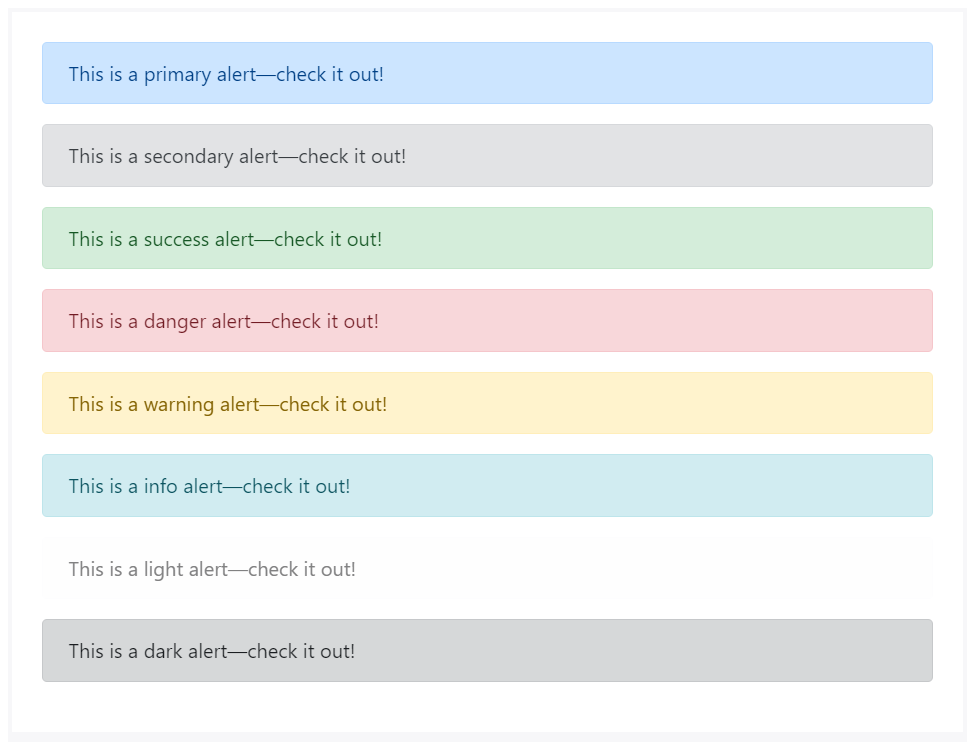
\includegraphics[scale=1.0]{alert_bootstrap.PNG}  
			\caption{Alert pada Bootstrap} 
		\end{figure}
		\begin{lstlisting}[frame=single] 
		<div class="alert alert-primary" role="alert">
		This is a primary alert—check it out!
		</div>
		<div class="alert alert-secondary" role="alert">
		This is a secondary alert—check it out!
		</div>
		<div class="alert alert-success" role="alert">
		This is a success alert—check it out!
		</div>
		<div class="alert alert-danger" role="alert">
		This is a danger alert—check it out!
		</div>
		<div class="alert alert-warning" role="alert">
		This is a warning alert—check it out!
		</div>
		<div class="alert alert-info" role="alert">
		This is a info alert—check it out!
		</div>
		<div class="alert alert-light" role="alert">
		This is a light alert—check it out!
		</div>
		<div class="alert alert-dark" role="alert">
		This is a dark alert—check it out!
		</div>
		\end{lstlisting}
		
		\myparagraph{Plugin}
		\colorbox{mygray}{\texttt{DateTimePicker}} dengan menggunakan jQuery untuk memilih tanggal dan waktu pada bagian forms. 
		\myparagraph{Inline DateTimePicker}
		Penggunaan plugin ini, memungkinkan \textit{users} untuk memilih tanggal dan waktu secara bersamaan.
		\begin{figure} [H]
			\centering  
			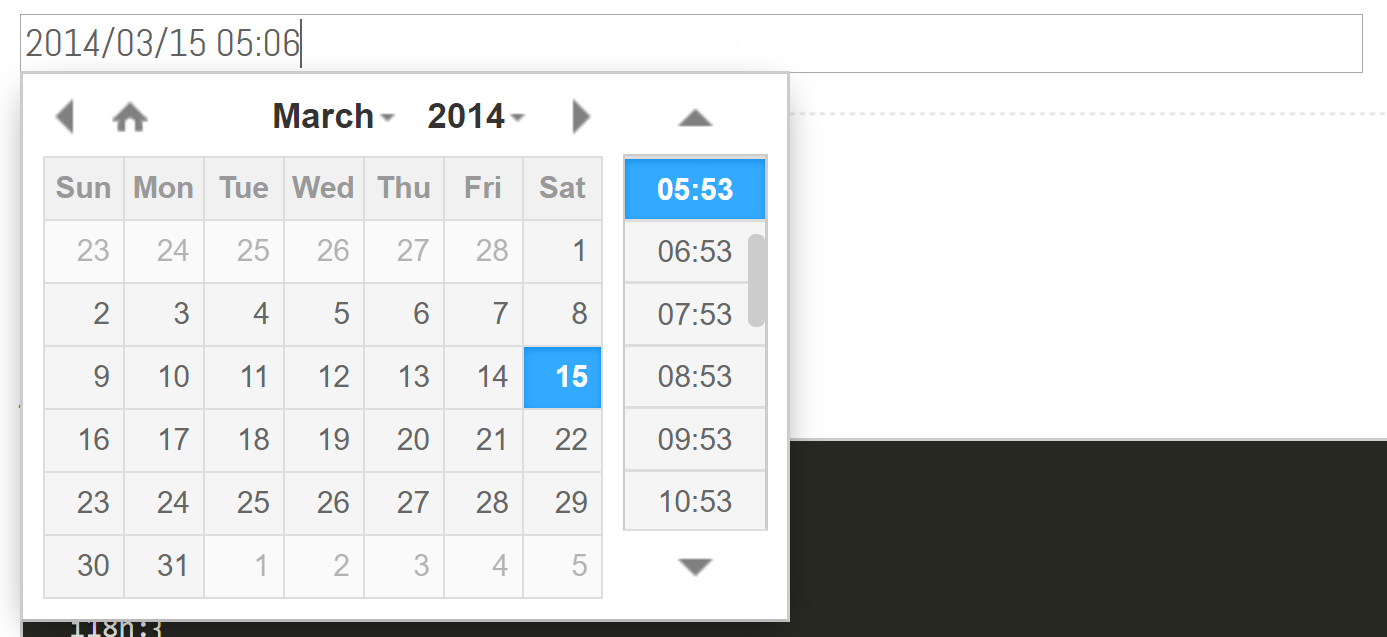
\includegraphics[scale=1.0]{datetimepicker_bootstrap4.PNG}  
			\caption{Datetimepicker pada Bootstrap} 
		\end{figure}
		\noindent Penggunaan nya dalam kode HTML sebagai berikut :
		\begin{lstlisting}[frame=single] 
		<input id="datetimepicker" type="text" >
		\end{lstlisting}
		
		\noindent Penggunaan dalam kode Javascript sebagai berikut :
		\begin{lstlisting}[frame=single] 
		jQuery('#datetimepicker').datetimepicker();
		\end{lstlisting}
		
		
		\item \textbf{Membuat rancangan tampilan website dan template.}\\
		{\bf Status :} Ada sejak rencana kerja skripsi.\\
		{\bf Hasil :} Belum diimplementasikan.
		
		\item \textbf{Mengimplementasikan keseluruhan rancangan tampilan dan template.}\\
		{\bf Status :} Ada sejak rencana kerja skripsi.\\
		{\bf Hasil :} Sebagian besar tampilan sudah diimplementasi. \\
		Berikut ini link perubahannya : \\
		\url{https://github.com/ftisunpar/BlueTape/compare/master...hapsarilw:master}
		
		\item \textbf{Menganalisis website BlueTape.}\\
		{\bf Status :} Baru dibuat saat ini.\\
		{\bf Hasil :}  \\
		
		
		\chapter{Analisis}
		Proyek BlueTape dijalankan menggunakan \textit{framework front-end}  Foundation. Secara garis besar, file-file yang berkaitan dengan Foundation seperti file javascript dan css akan dipanggil di file \textbf{BlueTape/www/application/views/templates/script{\_}foundation.php} dan \textbf{BlueTape/www/application/views/templates/head{\_}loggedin.php}. Kemudian penggunaan komponen Foundation terdapat pada file-file main.php yang terletak di setiap modul pada folder \textbf{BlueTape/www/application/views/} beserta kegunaan nya pada website.
		\myparagraph{Analisis Frontend Library}
		\myparagraph{Foundation}
		Dalam proyek BlueTape, file Foundation tersimpan di folder js dan css. Foundation yang digunakan pada projek ini adalah versi 6.1.2. Detail komponen yang digunakan adalah sebagai berikut :
		\begin{enumerate}
			\item \colorbox{mygray}{\texttt{.row}}
			\begin{itemize}
				\item Untuk membuat konten yang terletak di dalam satu baris untuk setiap halaman website.
				\item Untuk memisahkan baris dari sekumpulan field dalam sebuah form.
			\end{itemize}
			\item \colorbox{mygray}{\texttt{.column}}
			\begin{itemize}
				\item Membuat kolom untuk menampung konten
				\item Membuat kolom pada field dalam form
			\end{itemize}	
			\item \colorbox{mygray}{\texttt{<table>}}  \par
			\begin{itemize}
				\item 	Seluruh tabel dalam proyek BlueTape memiliki format yang akan menyesuaikan posisinya dengan menampilkan data nya secara bertumpuk, sehingga dibutuhkan tag \colorbox{mygray}{\texttt{<table>}}dan kelas \colorbox{mygray}{\texttt{.stack}}. Tabel akan terdiri dari satu tag \colorbox{mygray}{\texttt{<thead>}} dan \colorbox{mygray}{\texttt{<tbody>}}.
				\item Bagian thead terdiri dari satu tag \colorbox{mygray}{\texttt{<tr>}} dan beberapa tag \colorbox{mygray}{\texttt{<th>}} yang membuat tulisan di dalam sel bersifat \texttt{bold}. Bagian tbody terdiri dari satu tag \colorbox{mygray}{\texttt{<tr>}} dan beberapa tag \colorbox{mygray}{\texttt{<td>}}. 
			\end{itemize}
			Tabel yang menggunakan kelas ini sebagai berikut :
			\begin{center}
				\begin{tabular}{||c | c | c||} 
					\hline
					Tabel & Modul & Keterangan \\ [0.5ex] 
					\hline\hline
					Daftar Jadwal &  Entri Jadwal Dosen &\\
					\hline
					Permohonan Perubahan Kuliah &  Perubahan Kuliah Manage &\\
					\hline
					Detail Permohonan  &  Perubahan Kuliah Manage & Modal dari Aksi Lihat\\
					\hline
					Histori Permohonan &  Perubahan Kuliah Request & \\
					\hline
					Permintaan Transkrip &  Transkrip Manage &\\
					\hline
					Detail Permohonan &   Transkrip Manage & Modal dari Aksi Lihat\\
					\hline
					Histori Permohonan &  Transkrip Request & Modal dari Aksi Lihat\\
					\hline	
				\end{tabular}
			\end{center}	
			\item Kelas \colorbox{mygray}{\texttt{.callout}} : Border untuk menampung setiap konten di website BlueTape seperti form dan tabel. 
			\item Kelas \colorbox{mygray}{\texttt{.large-*}}, \colorbox{mygray}{\texttt{.medium-*}} :
			\begin{itemize}
				\item Komponen medium-12 digunakan dalam callout, sehingga apabila layar berukuran sedang, callout akan memiliki lebar 12 grid.
				\item Sedangkan komponen  large-* digunakan untuk mengatur lebar suatu input field dalam satu form. Lebar field berbeda - beda tergantung presentase suatu input field dalam satu baris.
			\end{itemize} 
			\item Tag \colorbox{mygray}{\texttt{<form>}} : \par
			Ada dua jenis metode yang digunakan dalam \texttt{form} :
			\begin{itemize}
				\item POST : Digunakan untuk memasukan input user yang disertai oleh aksi yang memanggil suatu method tertentu dari controller. Dalam BlueTape form post digunakan untuk membuat request transkrip, setiap aksi untuk konfirmasi permohonan transkrip, permohonan baru  perubahan kuliah.
				\item GET : Digunakan untuk mencari permintaan transkrip berdasarkan NPM.
			\end{itemize}	  
			Atribut yang digunakan dalam website BlueTape : 	
			\begin{itemize}
				\item \colorbox{mygray}{\texttt{aria-label}} : digunakan untuk memberi keterangan pada input field dalam form.
				\item \colorbox{mygray}{\texttt{aria-hidden}} : digunakan ketika ingin mengambil data dari database atau data dari akun yang teregeristrasi.
				\item \colorbox{mygray}{\texttt{aria-selected}} : digunakan apabila input terdiri dari beberapa pilihan dan menggunakan empa
			\end{itemize}	
			\item Reveal
			Modal digunakan untuk menampilkan data tertentu berdasarkan aksi yang dipilih. Terdapat empat aksi yang menggunakan modal yaitu modal lihat, setuju, tolak dan hapus.
			\begin{itemize}
				\item Modal memiliki kelas \colorbox{mygray}{\texttt{.reveal}} dan atribut \colorbox{mygray}{\texttt{data-reveal}}.
				\item Setiap modal akan memiliki tombol hapus. Penggunaan kelas \texttt{.close-button} dan atribut \colorbox{mygray}{\texttt{data-close}} akan diaplikasikan.			
			\end{itemize} 	 
		\end{enumerate}
		\myparagraph{Template Flash Message}
		File ini terletak di \textbf{BlueTape/www/application/views/templates/flashmessage.php}, disini akan diletakkan tampilan alerts yang terdiri dari dua jenis :
		\begin{figure} [H]
			\centering  
			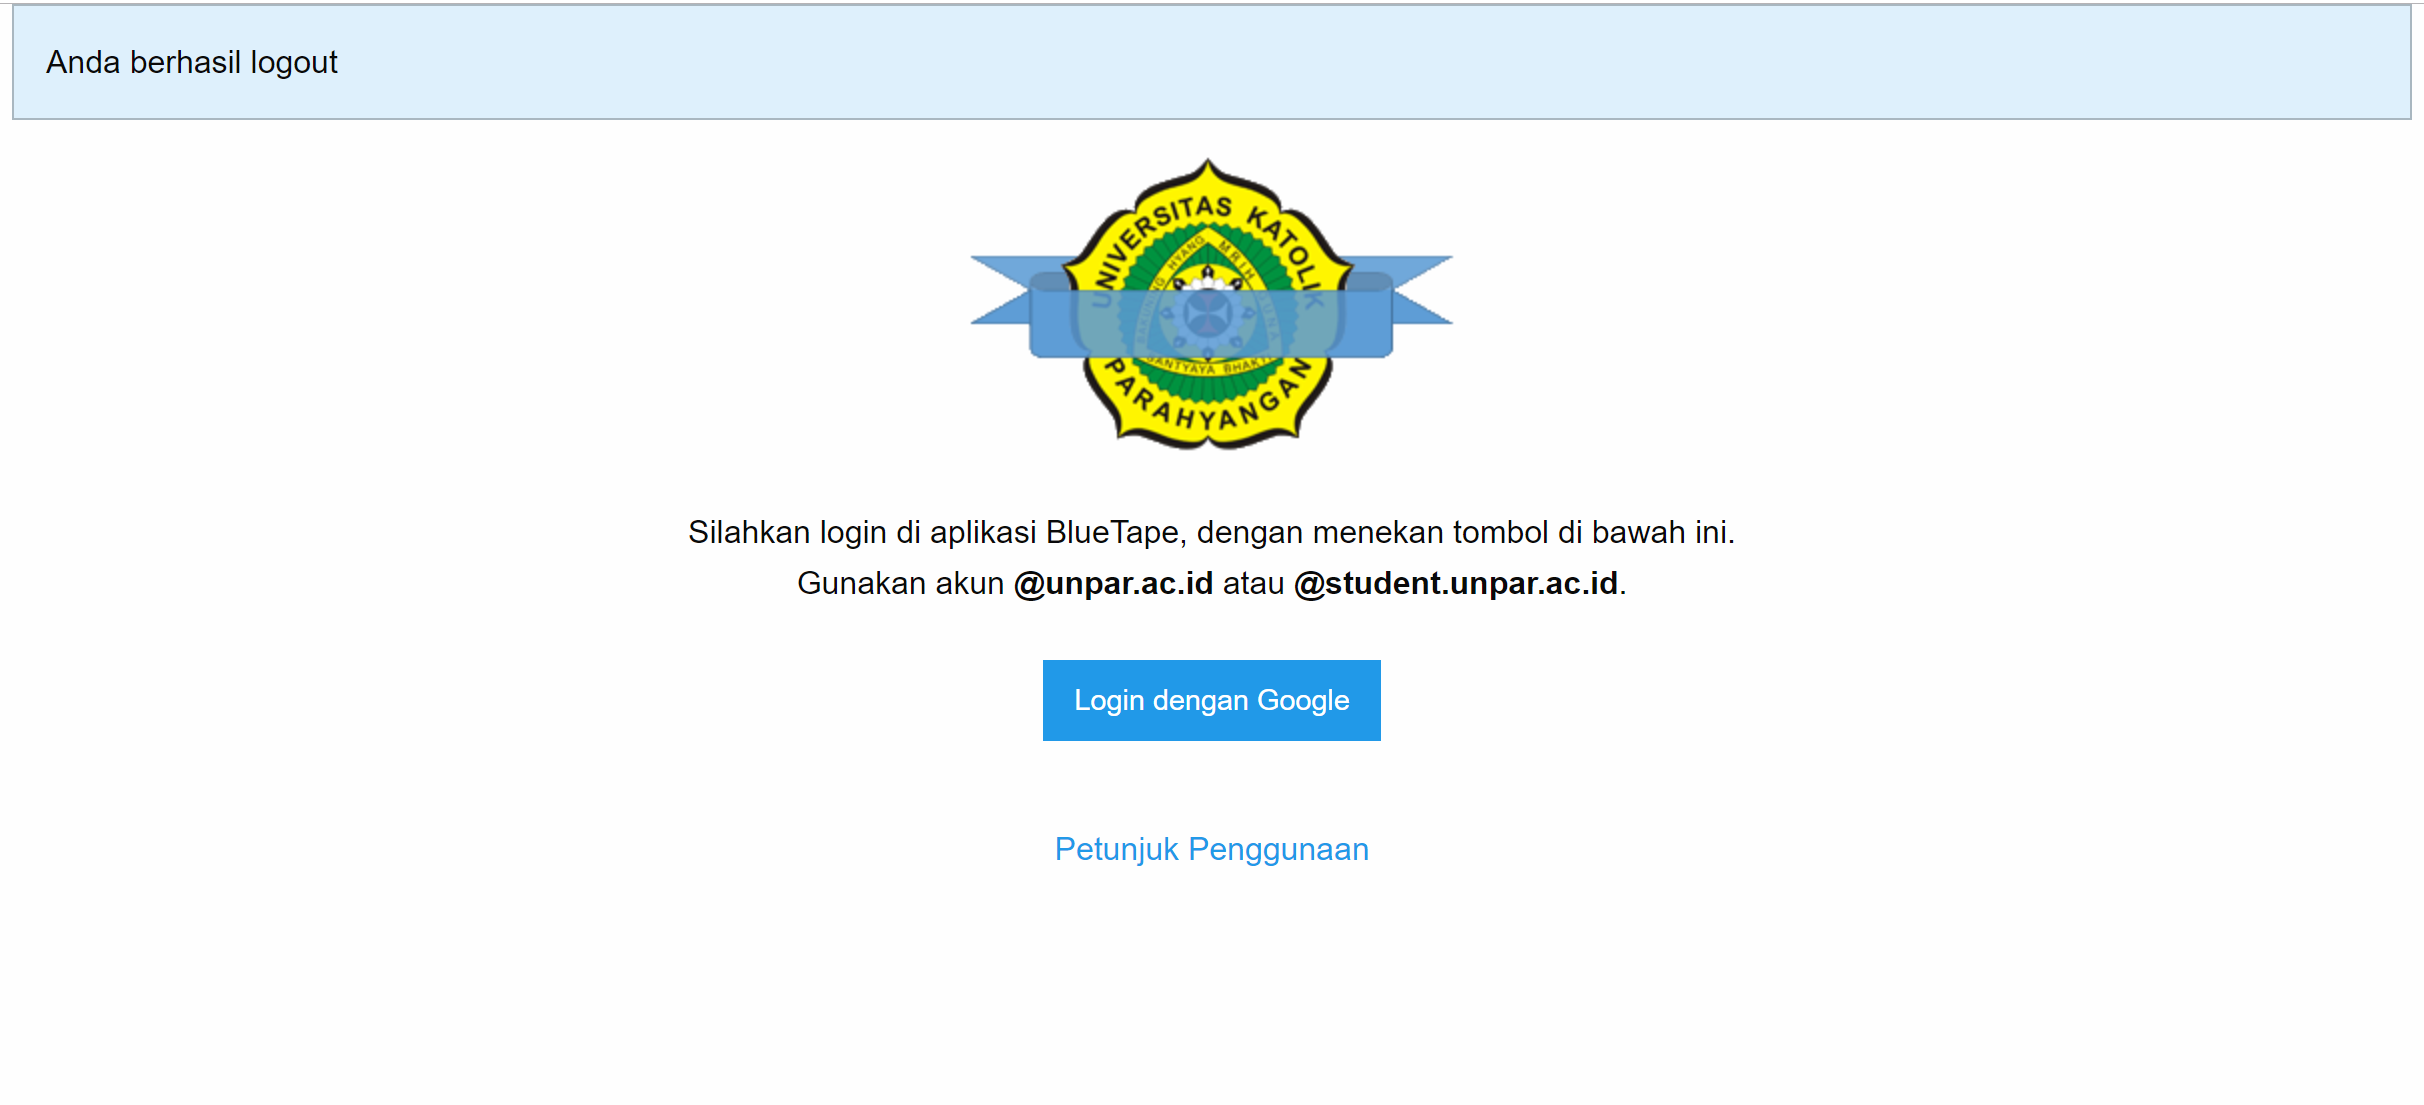
\includegraphics[scale=0.7]{alertInfo_zurb.png}  
			\caption{Alert mengenai 'info' pada BlueTape}	 
		\end{figure}
		
		\begin{figure} [H]
			\centering  
			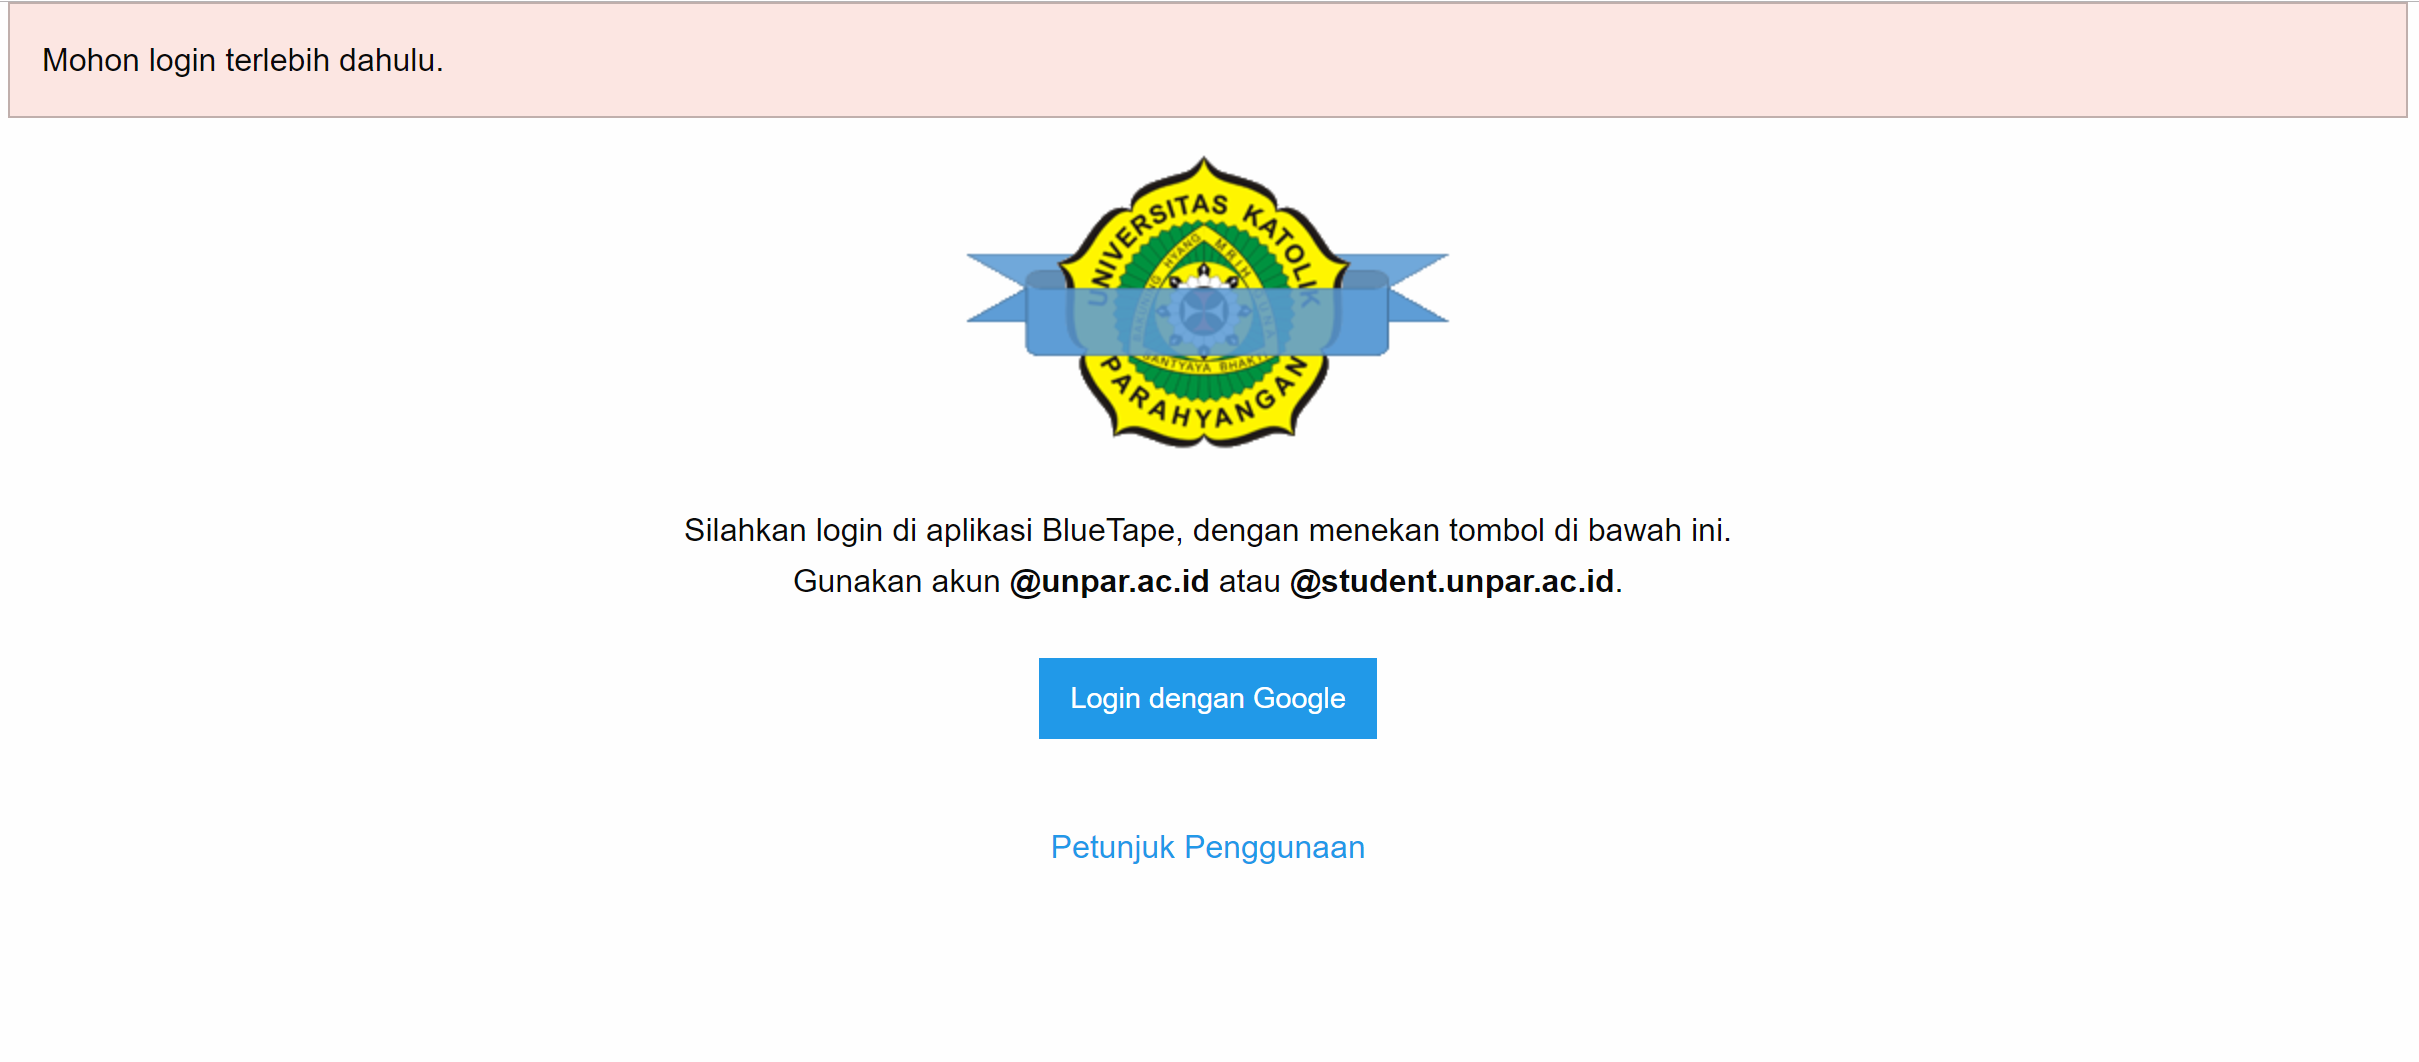
\includegraphics[scale=0.7]{alertError_zurb.png}  
			\caption{Alert mengenai 'error' pada BlueTape}	 
		\end{figure}
		\begin{enumerate}
			\item Alert 'error' : Penggunaan kelas \colorbox{mygray}{\texttt{.error}} akan membuat komponen \textit{alert} berwarna merah.
			\item Alert 'info' : Penggunaan kelas \colorbox{mygray}{\texttt{.alert}} akan membuat komponen \textit{alert} berwarna biru.
		\end{enumerate}
		
		\myparagraph{Template Head Logged In}
		File ini terletak di \textbf{BlueTape/www/application/views/templates/head\_loggedin.php}. Disini seluruh file css dari foundation dan plugin akan dimuat.
		
		\begin{figure} [H]
			\centering  
			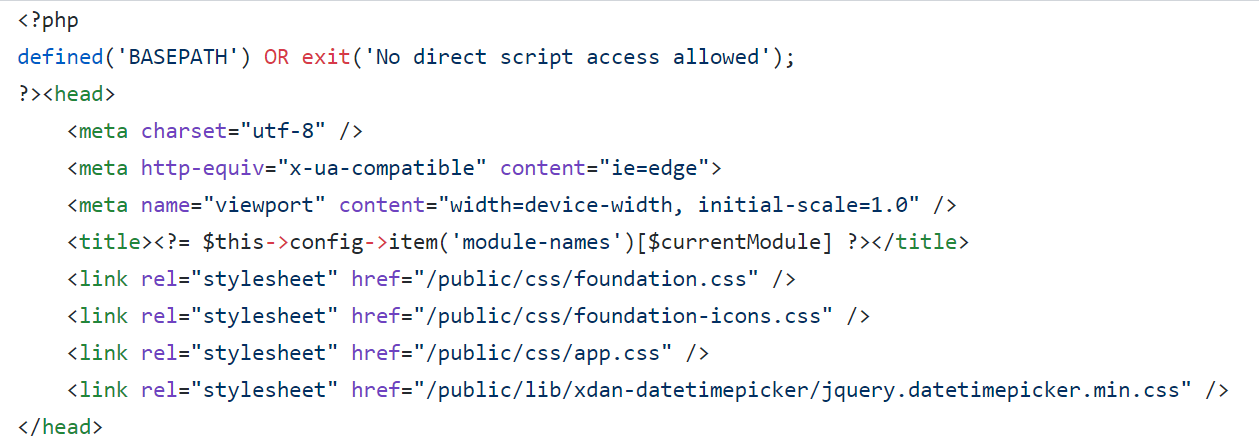
\includegraphics[scale=0.7]{head_loggedin.png}  
			\caption{Kode template untuk file head\_loggedin.php} 
		\end{figure}
		
		\myparagraph{Template Script Foundation}
		File ini terletak di \textbf{BlueTape/www/application/views/templates/script\_loggedin.php}.Disini seluruh file js dari foundation, jQuery dan plugin akan dimuat.
		
		\begin{figure} [H]
			\centering  
			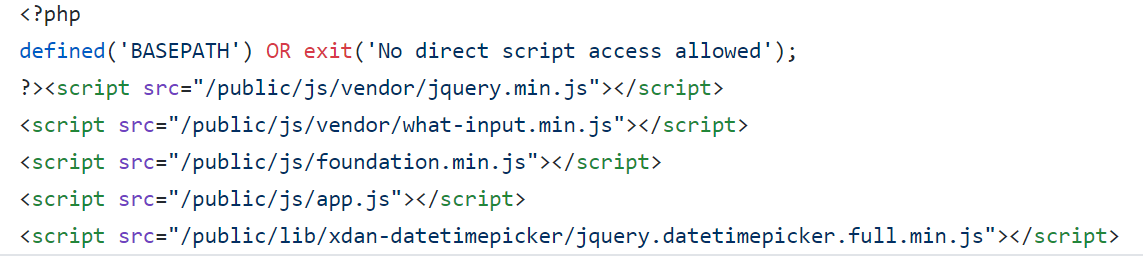
\includegraphics[scale=0.7]{script_foundation.png}  
			\caption{Kode template untuk file script_foundation.php} 
		\end{figure}
		\subsection{Template Top Bar Logged In}
		File ini terletak di \textbf{BlueTape/www/application/views/templates/topbar\_loggedin.php}.
		\begin{figure} [H]
			\centering  
			
\includegraphics[scale=0.5]{Tampilan_navbar_zurb.png}  
			\caption{Tampilan navbar dengan foundation} 
		\end{figure}
		\myparagraph{Antarmuka Cetak Transkrip}
		Antarmuka diaplikasikan pada file \textbf{BlueTape/www/application/views/TranskripRequest/main.php}. Isi dari halaman antarmuka cetak transkrip terdiri dari dua bagian yaitu :
		\begin{enumerate}
			\item \verb|Permohonan Baru| : Sistem akan memberikan dua tampilan untuk bagian ini, dengan kondisi sebagai berikut:
			\begin{itemize}
				\item Sistem akan menampilkan form pengajuan transkrip, apabila mahasiswa belum pernah mengajukan permohonan atau pengajuan sebelumnya  dikonfirmasi staf TU, maka mahasiswa dapat mengajukan permohonan baru.
				\item Sistem akan menampilkan informasi "Anda tidak bisa meminta cetak karena ada permintaan lain yang belum selesai", apabila mahasiswa memiliki pengajuan permohonan transkrip yang belum dikonfirmasi staf TU. 
			\end{itemize}
			\item \verb|Histori Permohonan| : Tabel untuk menampilkan informasi permohonan transkrip seorang mahasiswa. Status, tanggal pembuatan, tipe transkrip, tanggal cetak keterangan dan aksi. 
		\end{enumerate}
		Desain antarmuka sebagai berikut : \par
		Konten 'Permohonan Baru' dan 'Histori Permohonan' akan diletakkan pada satu \textit{row} yang memiliki kolom sebesar 12 grid pada layar medium dengan menggunakan komponen \colorbox{mygray}{\texttt{medium-12 column}}, untuk setiap konten nya akan dipisahkan oleh panel yang disebut dengan \texttt{callout}. \par
		Untuk konten Permohonan Baru :
		\begin{itemize}
			\item Bagian isi akan memiliki dua tampilan yaitu berbentuk form atau notifikasi yang berbentuk paragraf. Sehingga dibutuhkan komponen \verb|<form>| dan \verb|<p>|.
			\item Form terdiri dari dua baris yang dipisahkan oleh komponen \texttt{row}.
			\item Untuk field pada baris pertama akan memiliki kolom dengan panjang 4 grid. Sehingga dibutuhkan kelas \verb|large-4 column|. Jenis input yang digunakan bertipe email dan text. Selain itu untuk setiap input akan disertakan satu label sehingga menggunakan komponen \texttt{<label>}.
			\item Untuk field pada baris kedua memiliki dua jenis lebar grid yaitu 4 grid dan 8 grid. Sehingga membutuhkan kelas \verb|large-4 column|, \verb|large-8 column|. Untuk fied pada baris ketiga, tombol "Kirim Permohonan" memiliki \textit{background color} berwarna biru sehingga akan digunakan kelas \verb|button|.
		\end{itemize}
		Untuk konten "Histori Permohonan" :
		\begin{enumerate}	
			\item Pada kolom "Status" akan memiliki tiga jenis bentuk alert dengan \textit{backgroud} warna hijau, abu-abu dan merah. Sehingga dibutuhkan kelas \verb|warning|, \verb|success|, \verb|alert|.
			\item Aksi memiliki satu ikon "lihat" berwarna biru yang akan menampilkan sebuah modal. Sehingga dibutuhkan kelas ikon \verb|fi-eye|.
		\end{enumerate}
		\begin{figure} [H]
			\centering  
			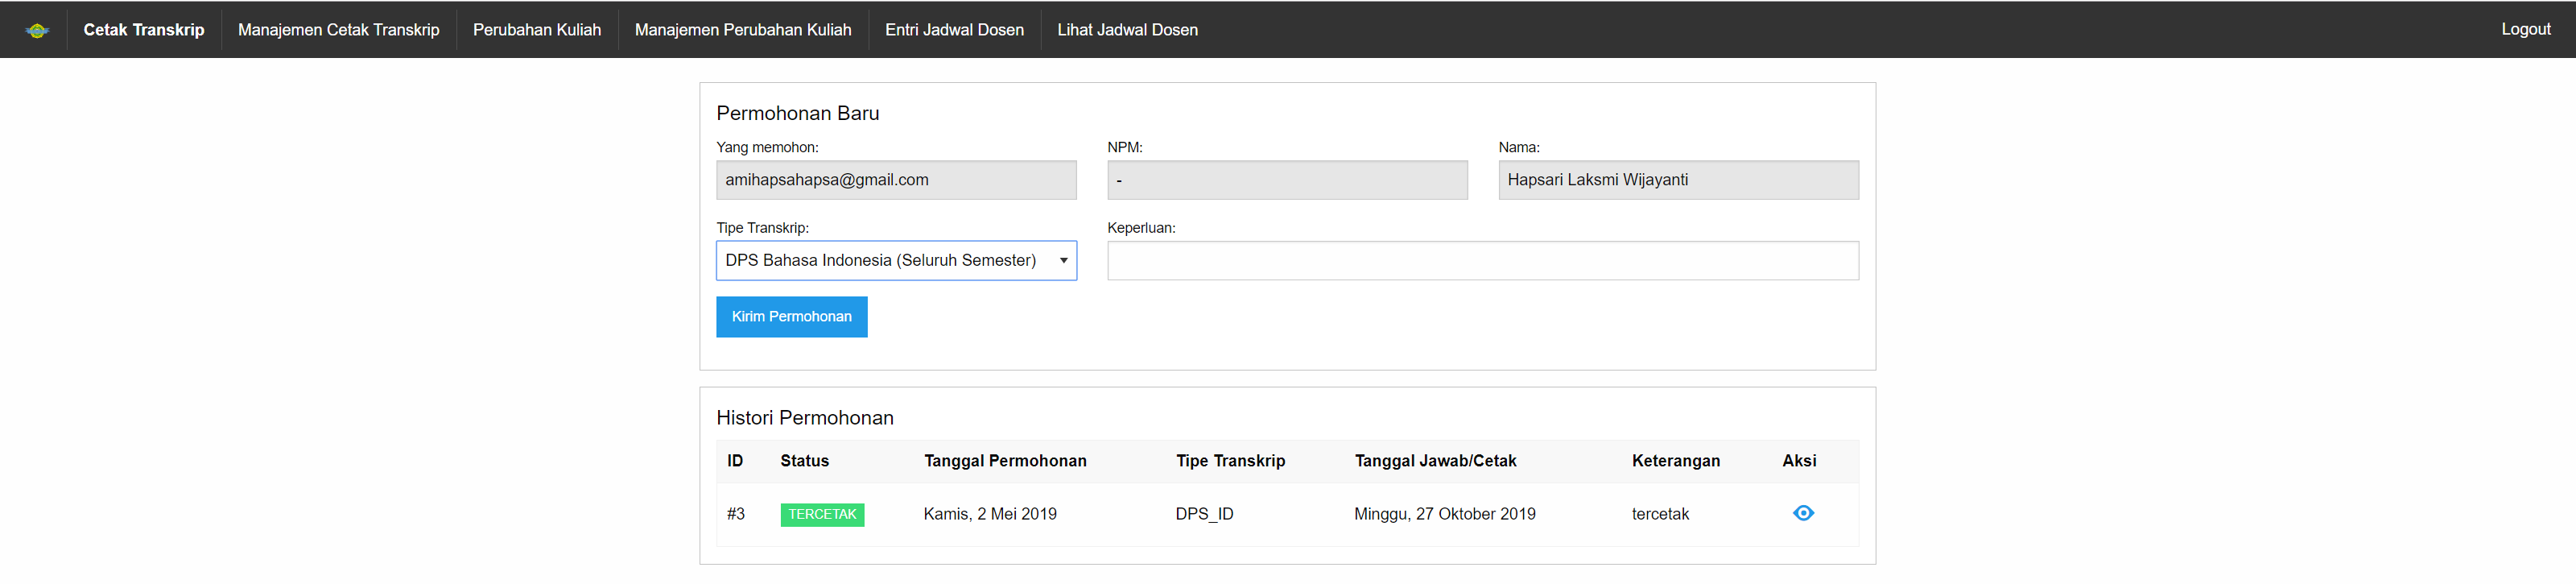
\includegraphics[scale=0.5]{Tampilan-Mahasiswa-Cetak-Transkrip.png}  
			\caption{Antarmuka Cetak Transkrip bagian 1} 
		\end{figure}
		\begin{figure} [H]
			\centering  
			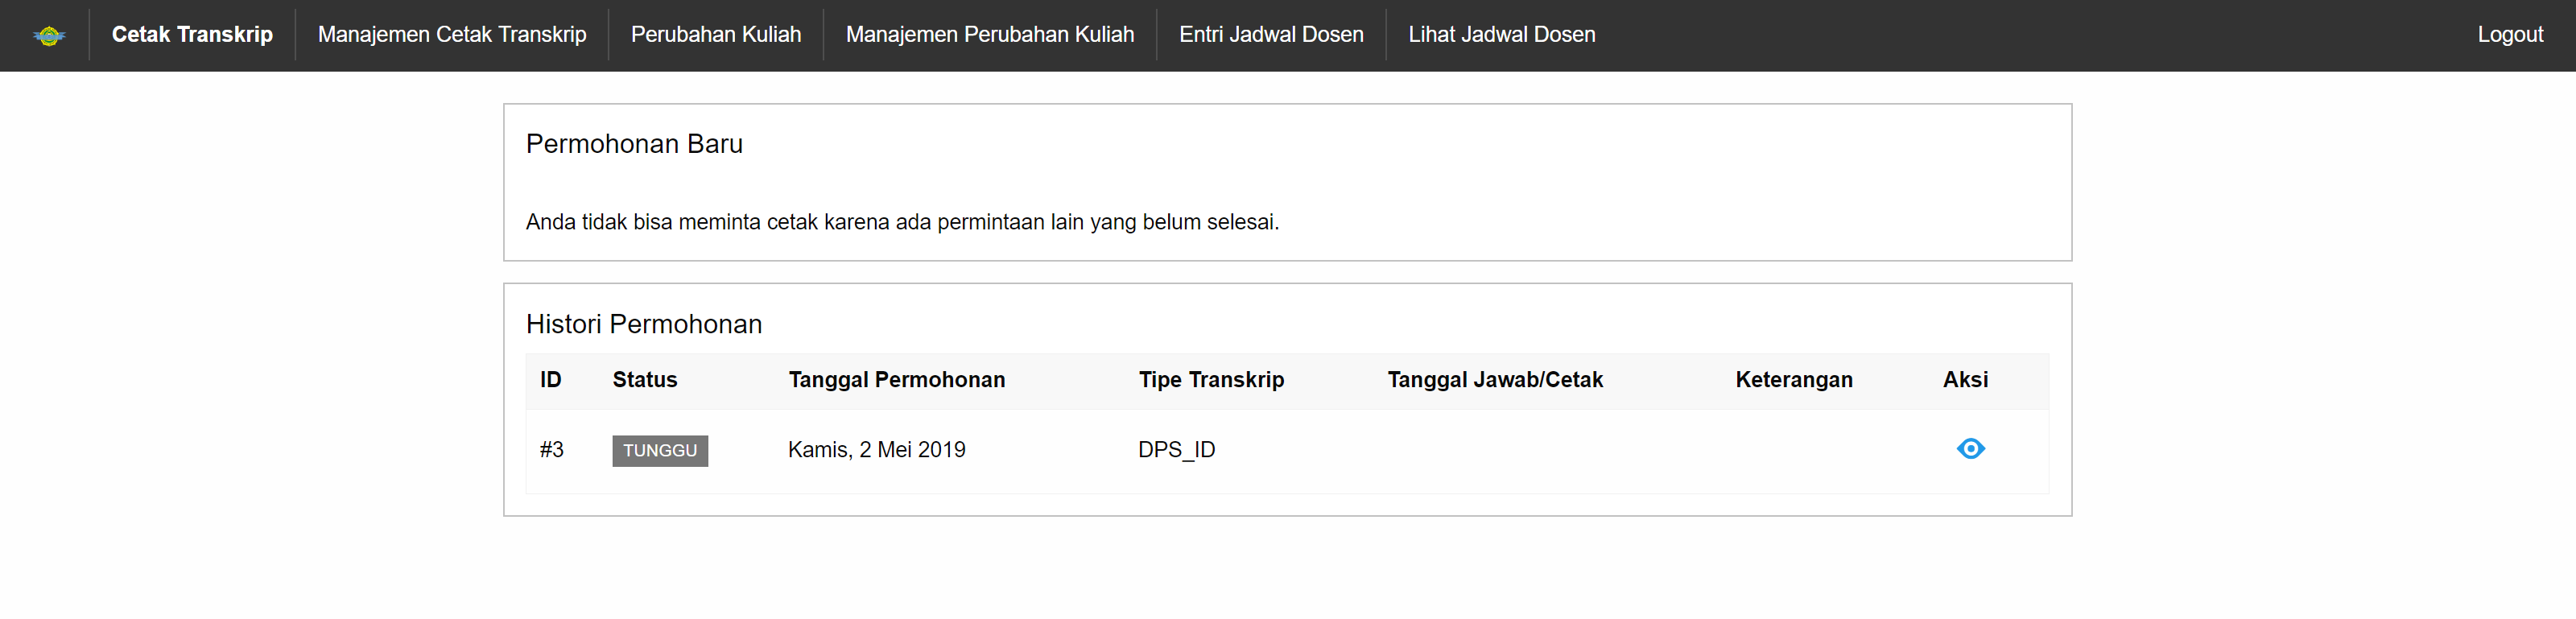
\includegraphics[scale=0.5]{Tampilan-Cetak-Transkrip.png}  
			\caption{Antarmuka Cetak Transkrip bagian 2} 
		\end{figure}
		Detail dari form permohonan baru, semua field akan disertai sebuah label untuk menjelaskan fungsi setiap field sehingga membutuhkan tag \texttt{<label>}  :
		\begin{itemize}	
			\item \texttt{Yang memohon} : Berisi email UNPAR mahasiswa, otomatis terisi saat login melalui gmail. Sehingga field tidak bisa diisi atau \textit{disabled} dibutuhkan atribut boolean \verb|readonly|
			\item \texttt{NPM} : Berisi NPM mahasiswa yang ter-\textit{generate} secara otomatis. Sehingga field tidak bisa diisi atau \textit{disabled} dibutuhkan atribut boolean \verb|readonly| dan \texttt{<input>} dengan tipe text.
			\item \texttt{Nama} : Nama mahasiswa yang tergenerate secara otomatis. Sehingga field tidak bisa diisi atau \textit{disabled} dibutuhkan atribut boolean \verb|readonly| dan \texttt{<input>} dengan tipe text.
			\item \texttt{Tipe Transkrip} : Terdiri dari tiga pilihan yaitu DPS Bahasa Indonesia(Seluruh Semester), DPS Bahasa Inggris(Seluruh Semester), LHS (Semester Terakhir). Wajib diisi. Tag \texttt{<select>} dan \texttt{<option>} yang \textit{value} nya diambil dari varibel \$type.
			\item Keperluan : Keterangan keperluan dibuat nya transkrip, wajib diisi mahasiswa. Menggunakan tag \texttt{<input>} dengan tipe text.
		\end{itemize}
		Apabila ada form yang belum diisi maka akan terdapat \textit{warning} untuk \textit{field} yang kosong.
		Berikut ini apabila mahasiswa menekan tombol aksi lihat 
\includegraphics[height=0.7\baselineskip]{tombol_eye.png} :
		\begin{figure} [H]
			\centering  
			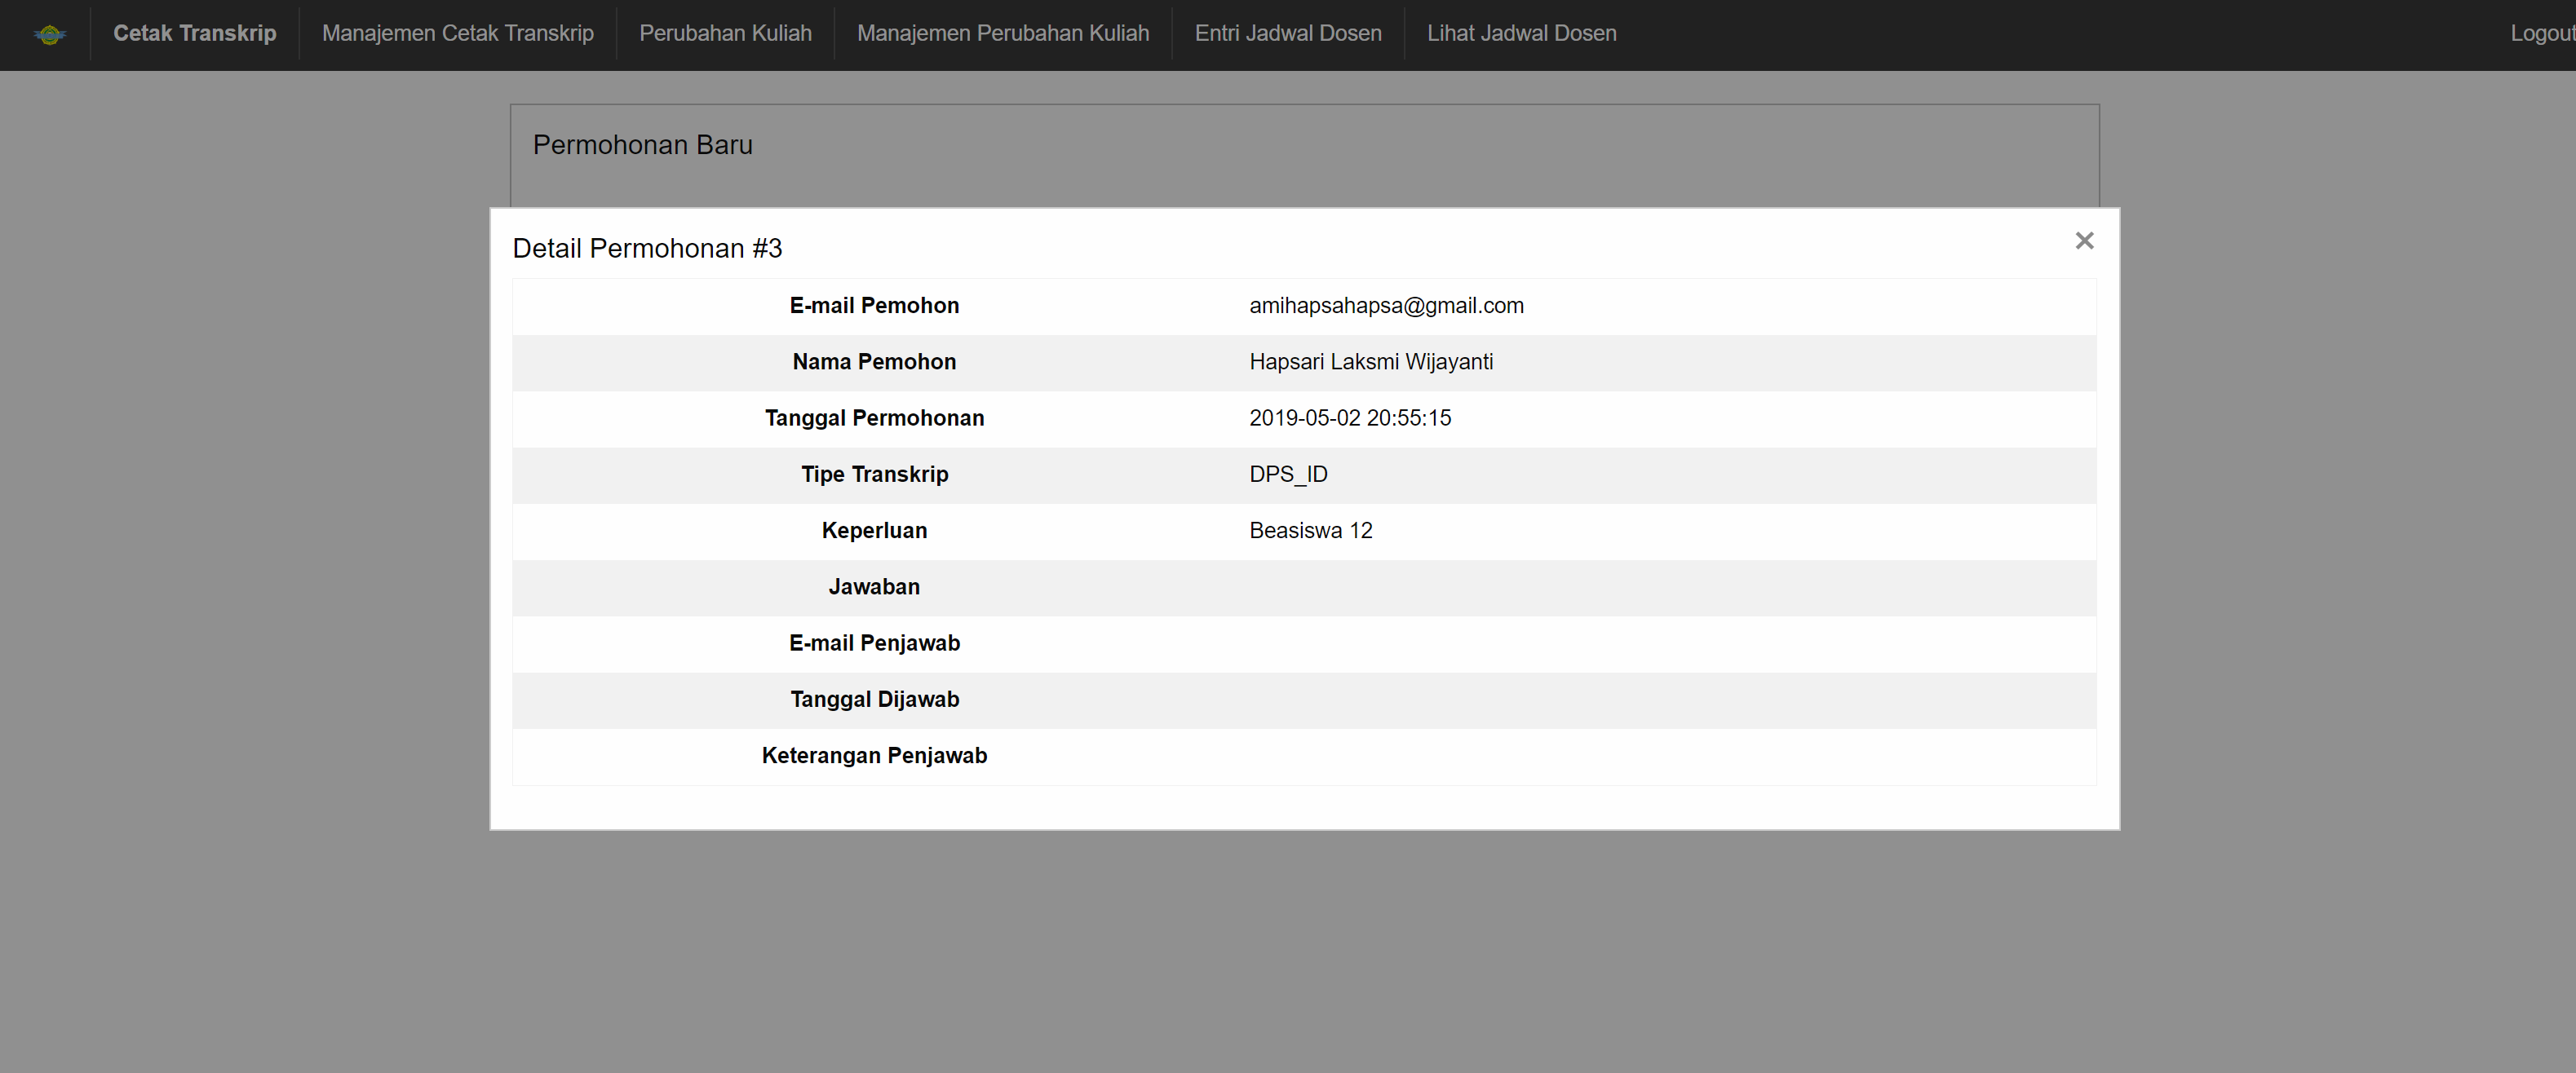
\includegraphics[scale=0.5]{Modal-Lihat-Cetak-Transkrip.png}  
			\caption{Modal Lihat Cetak Transkrip} 
		\end{figure}
		\noindent Disini aksi 'lihat' akan menampilkan sebuah modal yang berisi sebuah tabel bergaris yang menyimpan informasi detil permohonan, baik detil informasi dari mahasiswa maupun konfirmasi dari staf Tata Usaha. Sehingga dibutuhkan kelas \verb|.reveal| dan atribut \verb|data-reveal|.
		
		\myparagraph{Antarmuka Manajemen Cetak Transkrip}
		Antarmuka diaplikasikan pada file \textbf{BlueTape/www/application/views/TranskripManage/main.php}.
		\begin{figure} [H]
			\centering  
			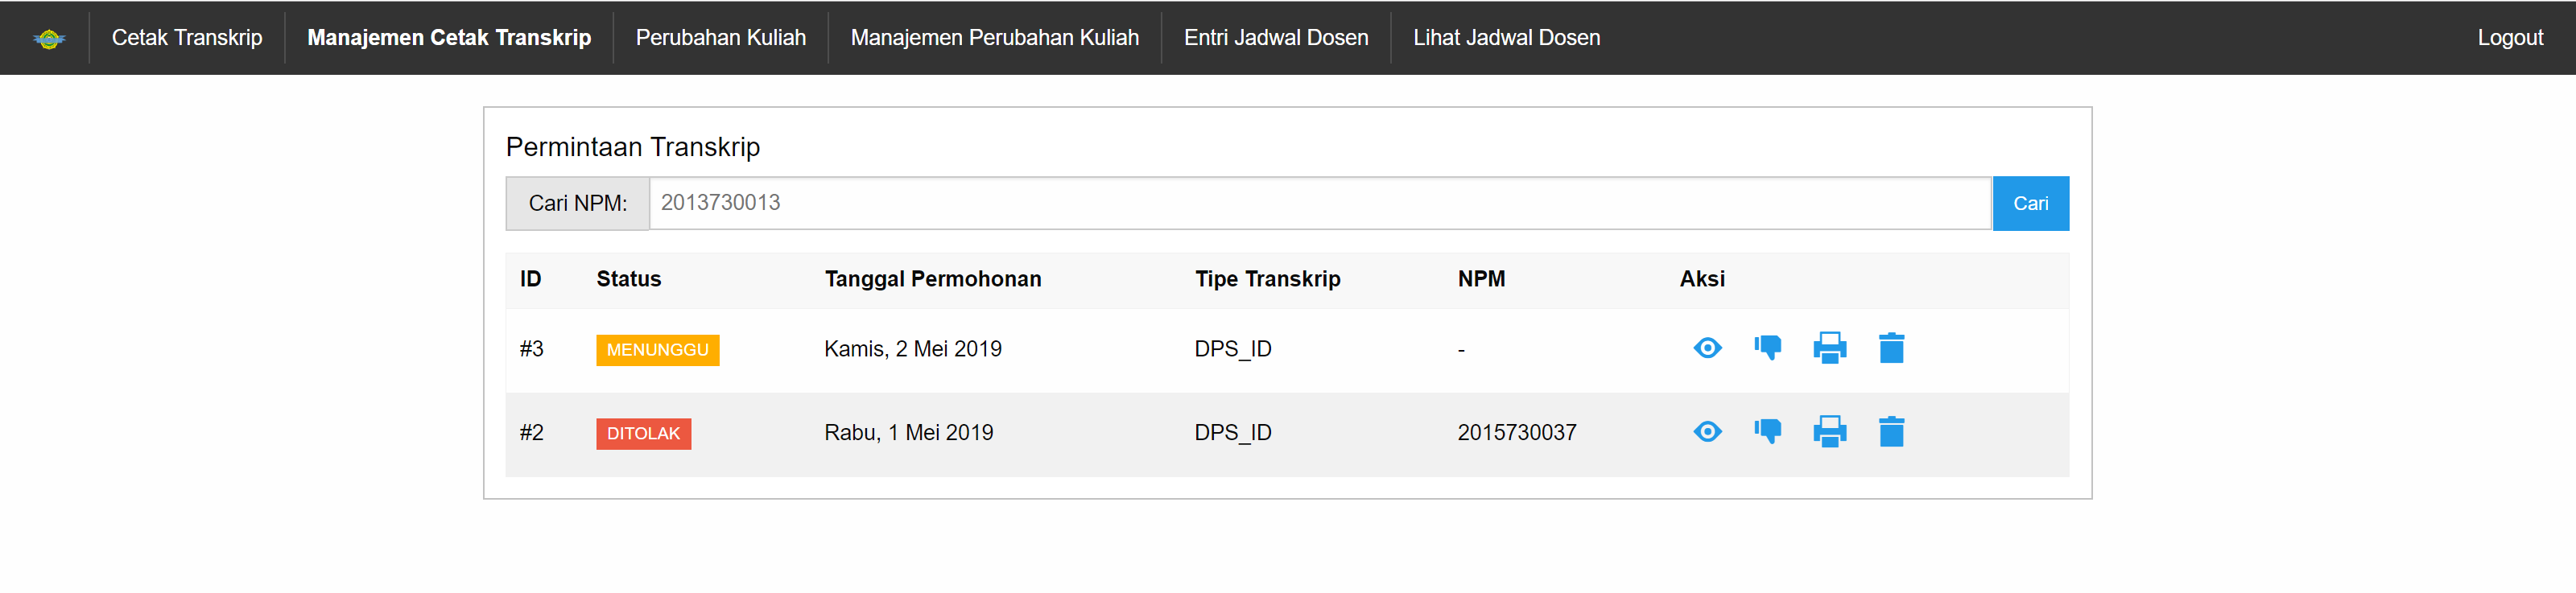
\includegraphics[scale=0.5]{Tampilan-Manajemen-Cetak-Transkrip.png}  
			\caption{Tampilan Manajemen Cetak Transkrip} 	
		\end{figure}
		
		Tampilan Manajemen Cetak Transkrip berisi sebuah tabel permintaan transkrip yang terdiri dari daftar permintaan transkrip dan form pencarian transkrip berdasarkan NPM. \par
		
		\noindent Detail penjelasan untuk field 'Status' dan 'Aksi' :
		\begin{itemize}
			\item \texttt{Status} : Output terdiri dari tiga jenis label yaitu 'MENUNGGU'(berwarna kuning), 'DITOLAK' (berwarna merah) dan 'TERCETAK'(berwarna hijau).  Sehingga dibutuhkan kelas \colorbox{mygray}{\verb|secondary|}, \colorbox{mygray}{\verb|success|}, \colorbox{mygray}{\verb|alert|}. 
			\item \texttt{Aksi} : Terdiri dari empat ikon font-awesome yaitu \verb|fi-eye, fi-dislike, fi-print, fi-trash,| yang akan menampilkan modal berisi informasi yang sesuai dengan perintah.
		\end{itemize}
		Modal akan menggunakan kelas \texttt{reveal} dan atribut \texttt{data-reveal} Detail penjelasan untuk modal : 
		
		\begin{enumerate}
			
			\item Modal Lihat : Terdiri dari sebuah \texttt{table} yang menampilkan data permintaan transkrip. Ikon menggunakan kelas \texttt{fi-eye} dan menerapkan atribut \texttt{data-open} yang berisi method hapus menuju ID tertentu.
			
			\item Modal Tolak : Terdiri dari sebuah \texttt{form} yang memiliki method \texttt{POST} yang memanggil sebuah method "/TranskripManage/answer". Terdapat tiga tipe input yang digunakan yaitu \texttt{hidden, text, submit}. Pada input text untuk label Alasan Penolakan, menggunakan kelas "input-group-field". Lalu untuk input bertipe \texttt{submit} menggunakan kelas alert-button untuk membuat button berwarna merah. Ikon menggunakan kelas \texttt{fi-dislike} dan menerapkan atribut \texttt{data-open} yang berisi method tolak menuju ID tertentu.
			
			\item Modal Print : Terdiri dari sebuah form yang terdiri dari label, field dan tombol berwarna biru sehingga membutuhkan kelas \colorbox{mygray}{\verb|input-group-field|}. Ikon menggunakan kelas \colorbox{mygray}{\texttt{fi-print}} dan menerapkan atribut \colorbox{mygray}{\texttt{data-open}} yang berisi method cetak menuju ID tertentu.
			
			\item Modal Hapus : Terdiri dari sebuah form yang terdiri dari paragraf yang bersifat bold, beberapa input dan tombol berwarna merah sehingga membutuhkan kelas \colorbox{mygray}{\verb|<p>|}, \colorbox{mygray}{\texttt{<strong>}},\colorbox{mygray}{\texttt{<input>}}.Ikon menggunakan kelas \texttt{fi-trash} dan menerapkan atribut \texttt{data-open} yang berisi method hapus menuju ID tertentu.
		\end{enumerate}
		
		\begin{figure} [H]
			\centering  
			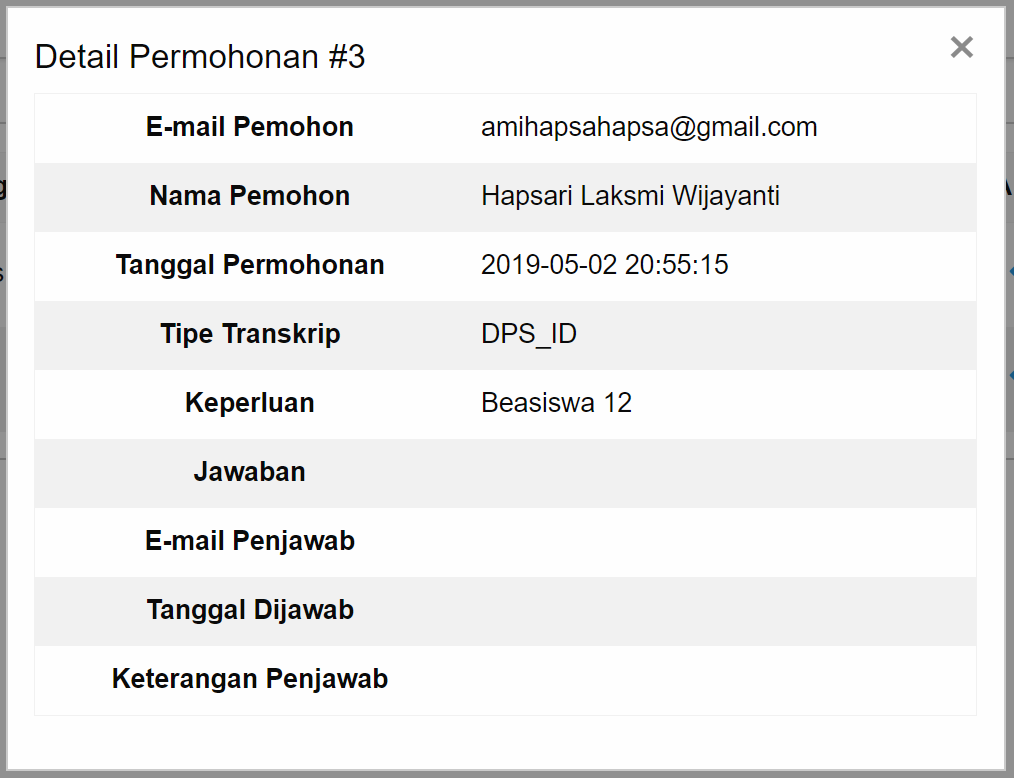
\includegraphics[scale=0.5]{Modal-Lihat-Manajemen-Cetak-Transkrip.png}  
			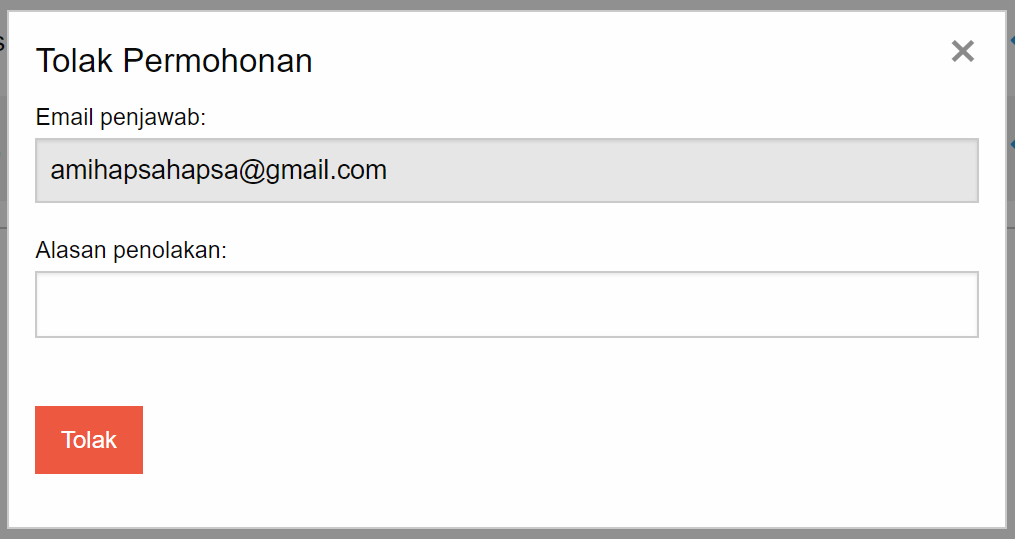
\includegraphics[scale=0.5]{Modal-Tolak-Manajemen-Cetak-Transkrip.png} 
			\caption{Tampilan Modal untuk aksi 'Lihat' dan 'Tolak'} 	
		\end{figure}
		
		\begin{figure} [H]
			\centering  
			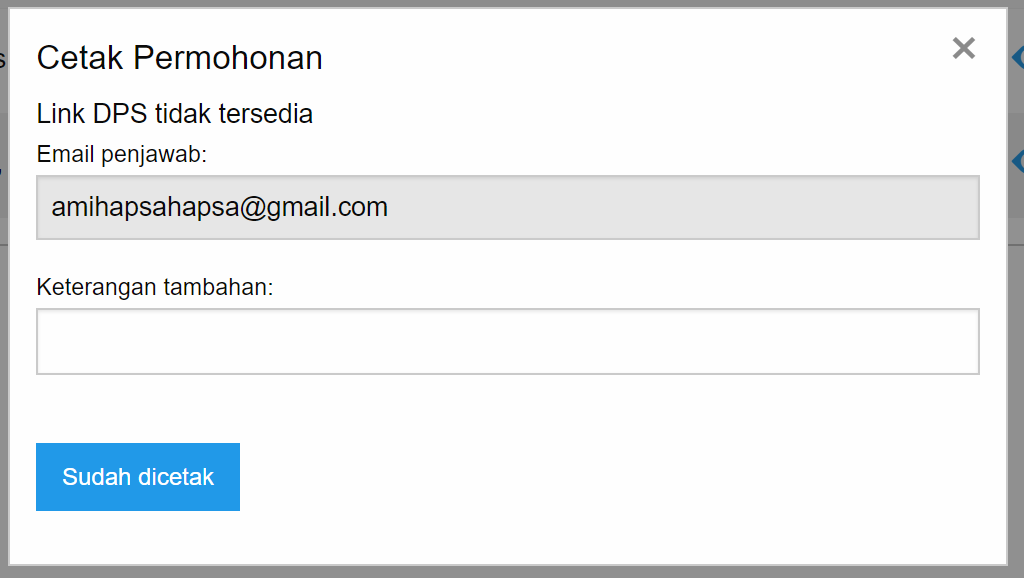
\includegraphics[scale=0.5]{Modal-Print-Manajemen-Cetak-Transkrip.png}  
			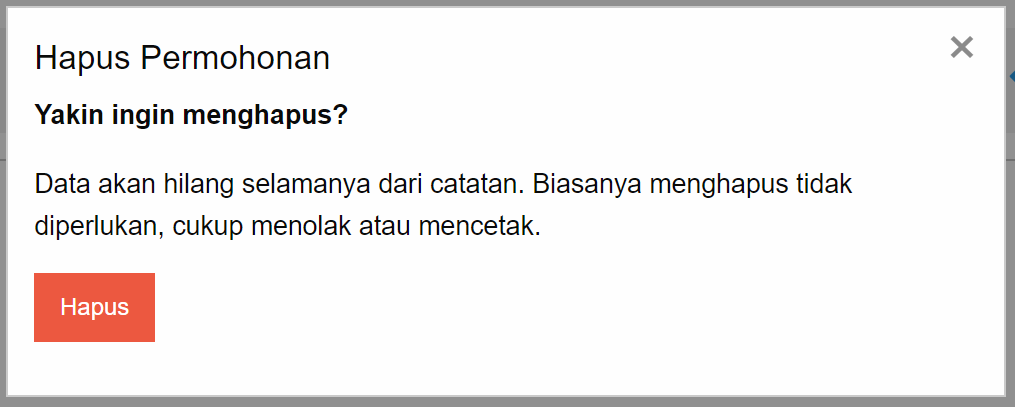
\includegraphics[scale=0.5]{Modal-Hapus-Manajemen-Cetak-Transkrip.png} 
			\caption{Tampilan Modal untuk aksi 'Print' dan 'Hapus'} 	
		\end{figure}
		
		
		\myparagraph{Antarmuka Perubahan Kuliah}
		Antarmuka diaplikasikan pada file \textbf{BlueTape/www/application/views/PerubahanKuliahRequest/main.php}.
		\begin{figure} [H]
			\centering  
			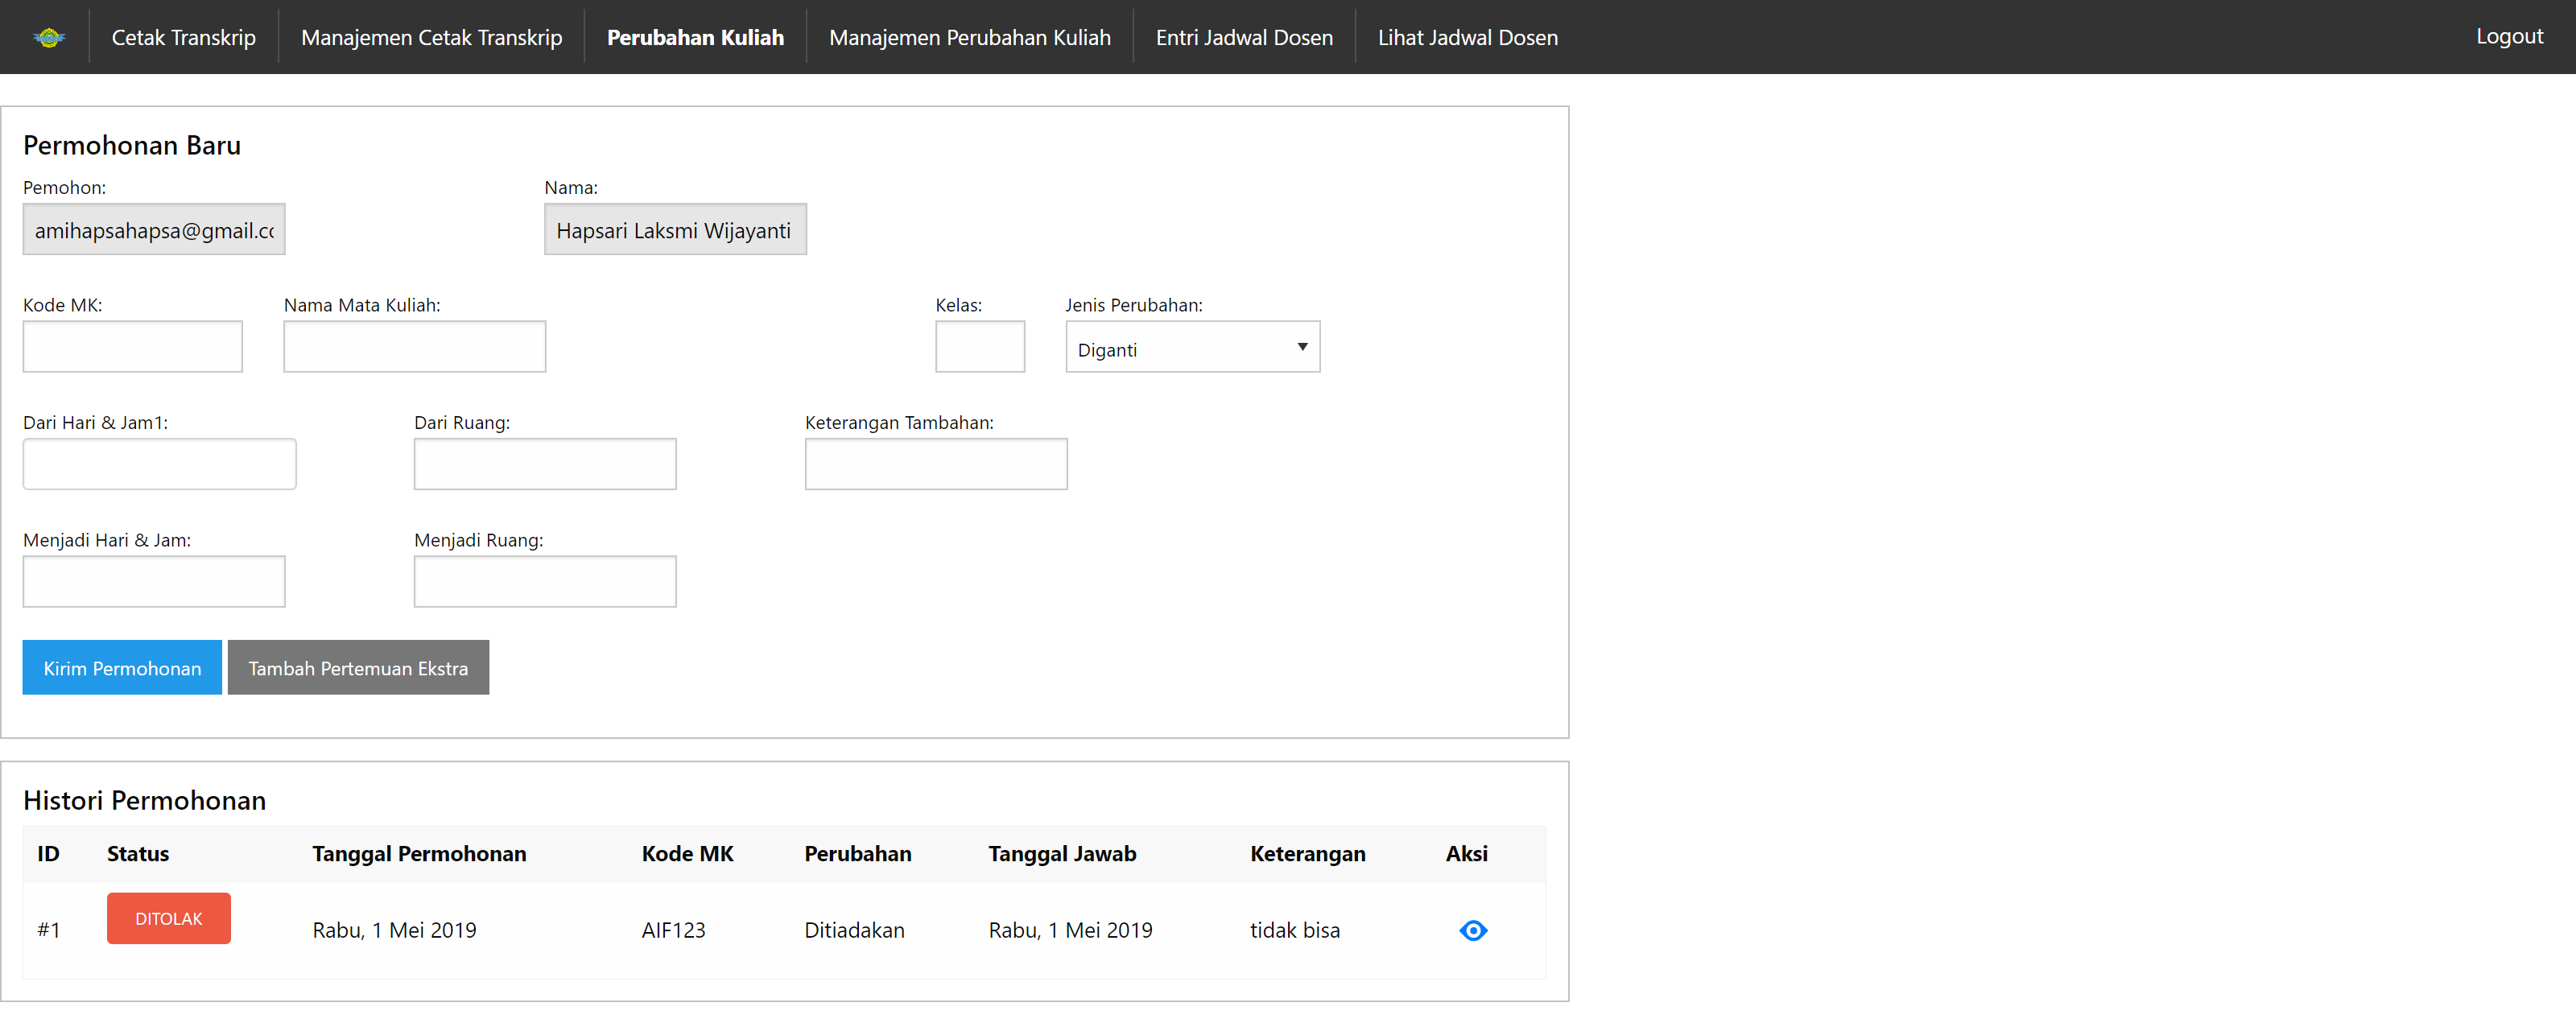
\includegraphics[scale=0.5]{Tampilan-Perubahan-Kuliah.png}  
			\caption{Tampilan Perubahan Kuliah} 
		\end{figure}
		
		Modul Perubahan Kuliah terdiri dari dua tabel yaitu :
		
		\myparagraph{Permohonan Baru}
		Permohonan baru diletakkan dalam sebuah row selebar 12 grid dan dikelilingi oleh sebuah border, membutuhkan kelas \colorbox{mygray}{\texttt{row}}, \colorbox{mygray}{\texttt{.large-12}}, \colorbox{mygray}{\texttt{column}} dan \texttt{callout}. Selain itu sebuah form dengan tipe \texttt{POST} akan ditampilkan untuk menyimpan masukan pemohon. Format dari form sebagai berikut :
		
		\myparagraph{Histori Pemohonan}
		Histori Permohonan menggunakan tabel yang bisa menyesuaikan lebarnya dengan menampilkan data secara bertumpuk sehingga menggunakan kelas \colorbox{mygray}{\texttt{.stack}}. Jenis data akan diletakkan dalam tag \\colorbox{mygray}{texttt{<thead>}} dalam satu baris sehingga menggunakan satu tag \colorbox{mygray}{\texttt{<tr>}} dan delapan tag \colorbox{mygray}{\texttt{<th>}}. Untuk bagian isi data menggunakan tag \colorbox{mygray}{\texttt{<tbody>}}.
		
		\begin{tabular}[!htbp]{ |p{4cm}|p{2cm}|p{10cm}|  }
			\hline
			Nama Kolom & Pilihan & Kelas Foundation yang digunakan\\
			\hline
			\texttt{Status} & dikonfirmasi, menggunakan kelas \colorbox{mygray}{\texttt{.success}} & Apabila staf TU menyetujui permohonanan\\
			\hline
			&  ditolak, menggunakan kelas \colorbox{mygray}{\texttt{.alert}}  & Apabila staf TU menolak permohonanan\\
			\hline
			& ditunggu, menggunakan kelas \colorbox{mygray}{\texttt{.secondary}} &  Apabila staf TU belum konfirmasi permohonan \\
			\hline
			\texttt{Tanggal Permohonan}    & & Data bertipe tanggal dengan format yang sudah ditentukan\\
			\hline
			\texttt{Kode MK} &  & Data berbentuk text \\
			\hline
			\texttt{Perubahan} &  & Data berbentuk text \\
			\hline
			\texttt{Tanggal Jawab} &  & Data bertipe tanggal \\
			\hline
			\texttt{Keterangan} &  & Data berbentuk text \\
			\hline
			\texttt{Aksi} &  & Terdapat tombol aksi 'Lihat', menggunakan font awesome dan kelas \colorbox{mygray}{\texttt{fas fa-eye}} yang akan memanggil sebuah modal sesuai id yang diinginkan user. Untuk modal, menggunakan kelas \texttt{reveal} dan atribut \colorbox{mygray}{\texttt{data-reveal}}\\
			\hline
		\end{tabular}
		Ketika user menekan tombol aksi 'lihat', maka modal berisi sebuah tabel informasi data permohonan akan ditampilkan sesuai dengan ID.
		\begin{figure} [H]
			\centering  
			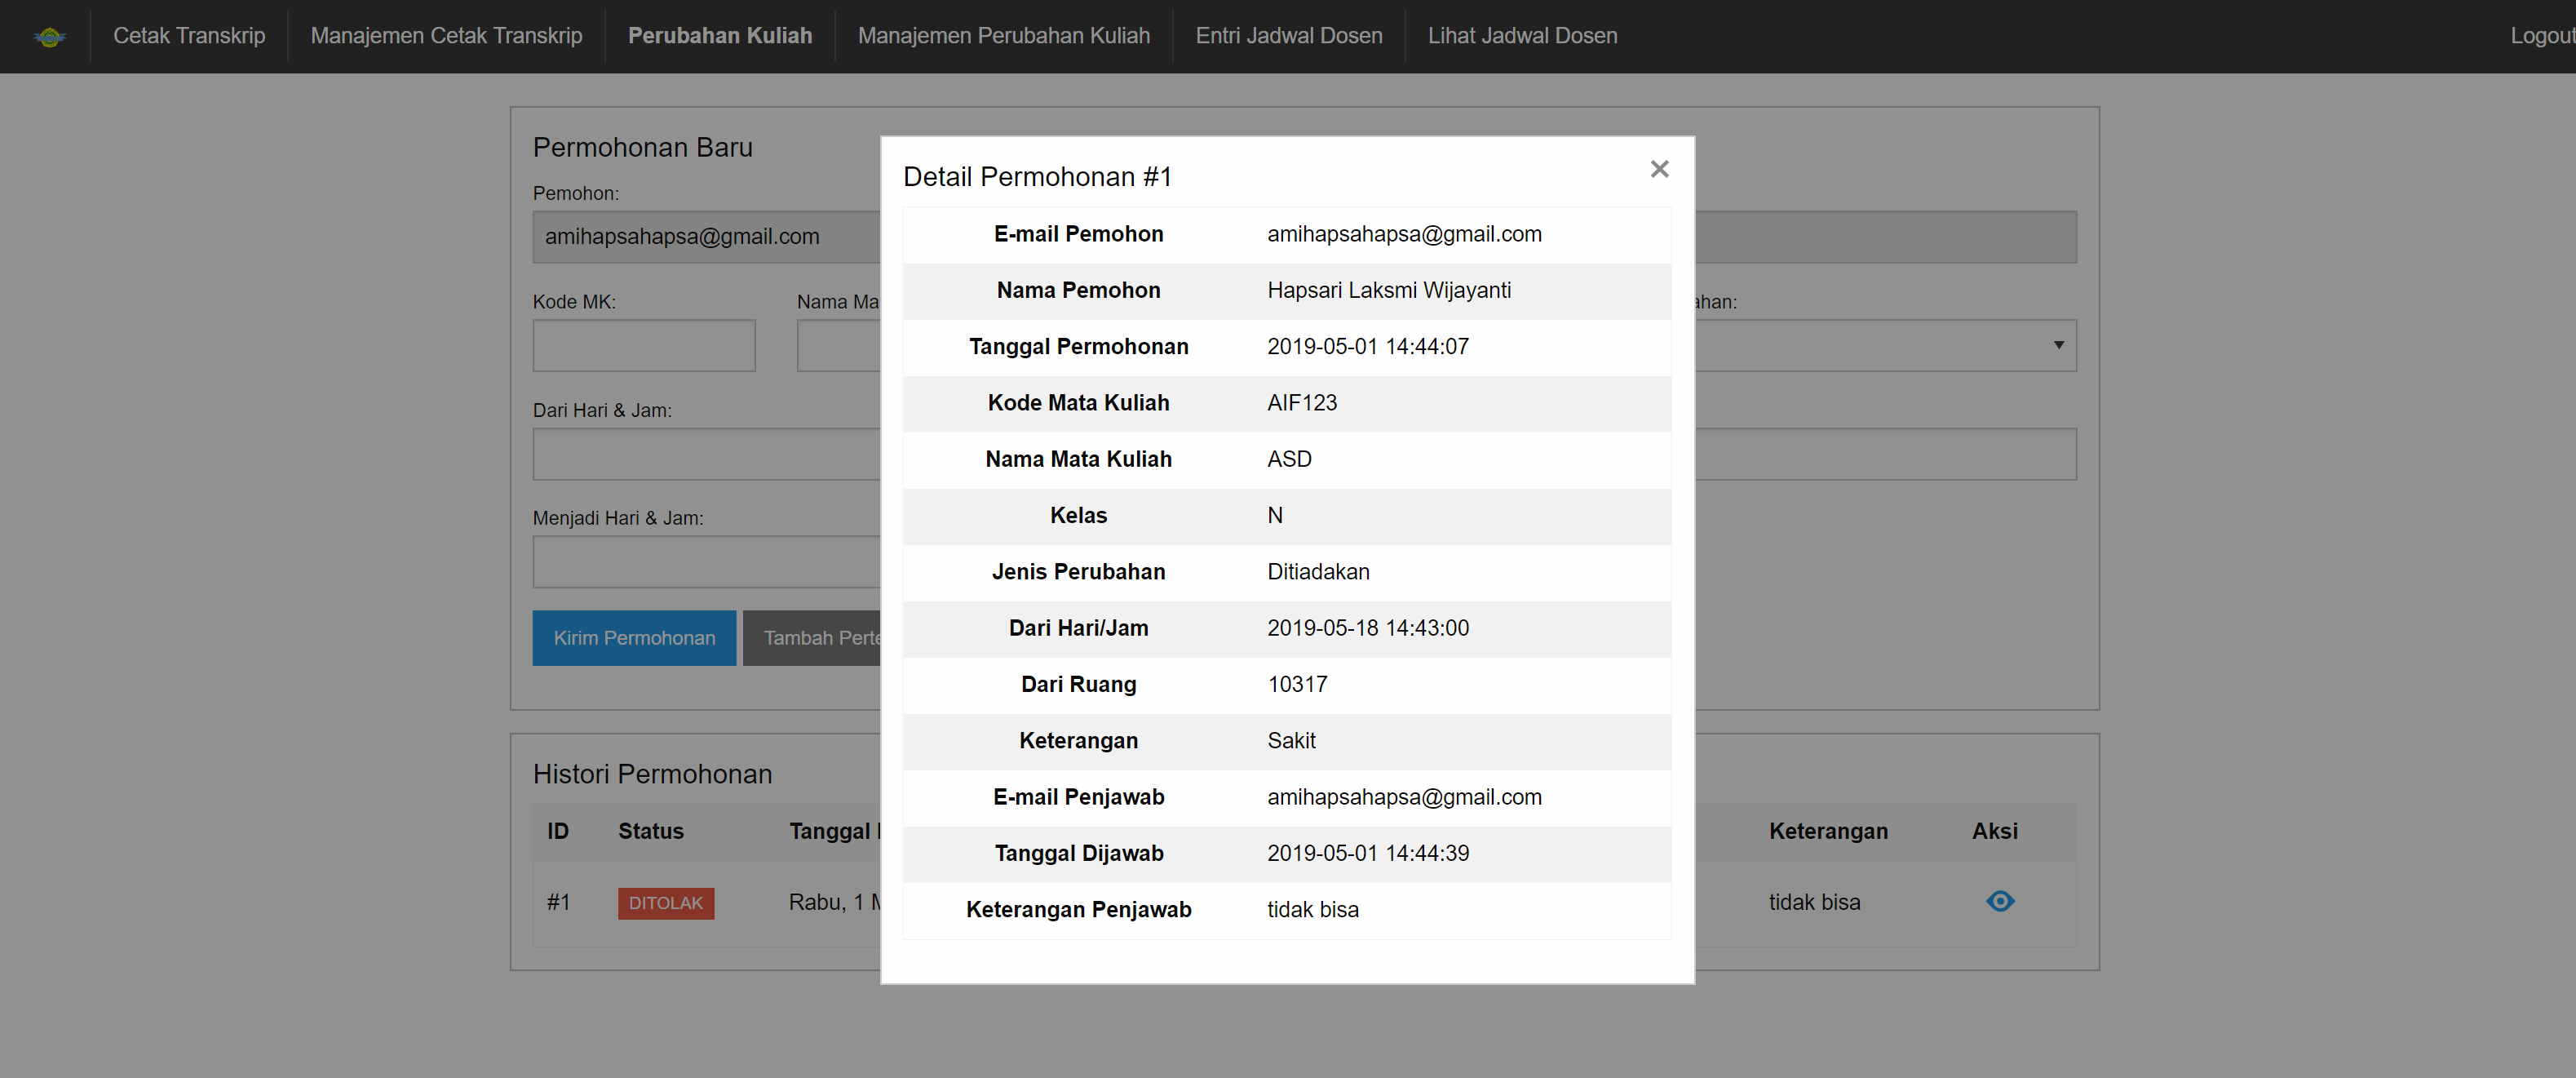
\includegraphics[scale=0.5]{Modal-Lihat-Perubahan-Kuliah.png}  
			\caption{Modal Lihat Perubahan Kuliah} 
		\end{figure}
		
		\myparagraph{Antarmuka Manajemen Perubahan Kuliah}
		Antarmuka diaplikasikan pada file \textbf{BlueTape/www/application/views/PerubahanKuliahManage/main.php}.
		\begin{figure} [H]
			\centering  
			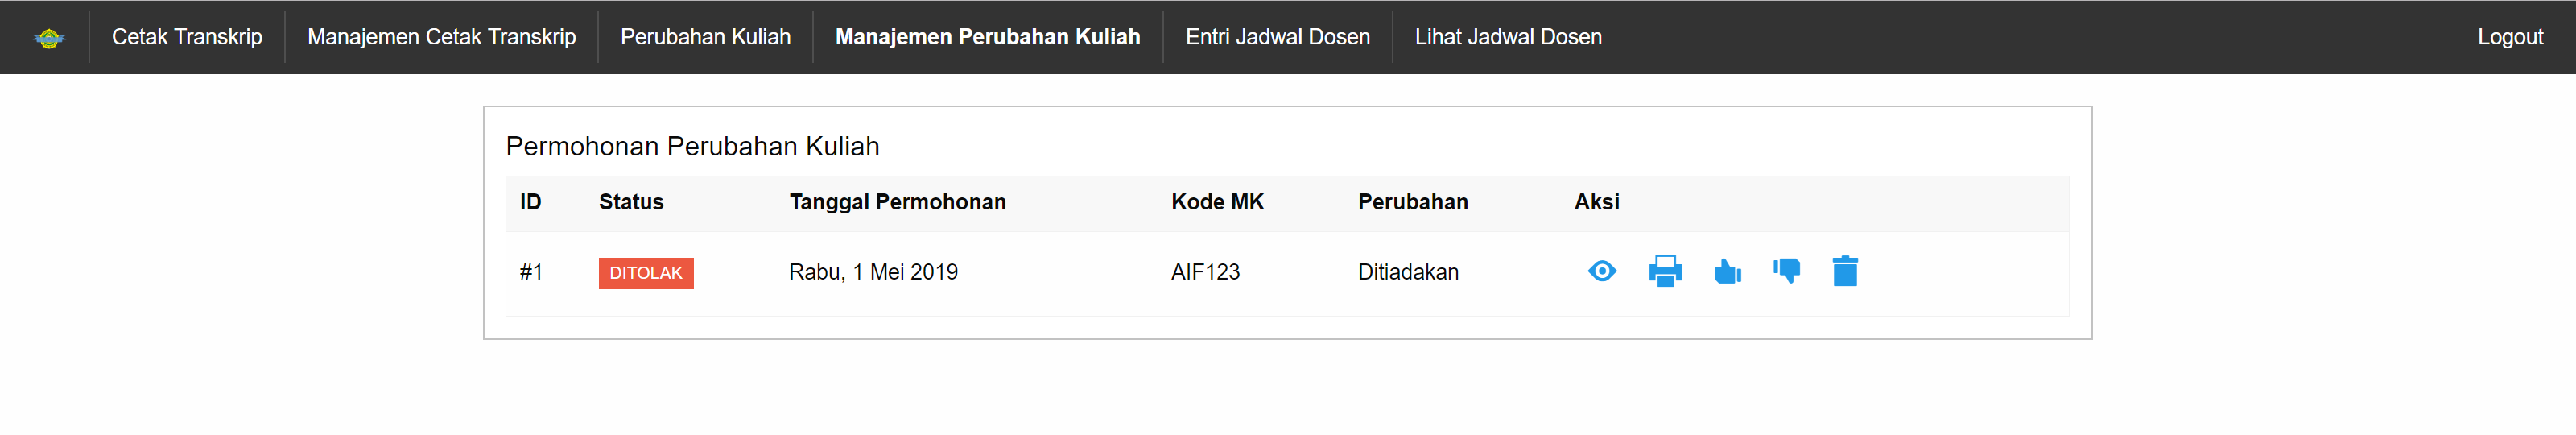
\includegraphics[scale=0.5]{Tampilan-Manajemen-Perubahan-Kuliah.png}  
			\caption{Tampilan Manajemen Perubahan Kuliah} 
		\end{figure}
		Tabel Pemohonan Kuliah memiliki detail yang sama dengan tabel histori permohonan, namun aksi yang dilakukan terdiri dari lima perintah:
		
		\begin{tabular}{|p{4cm}|p{2cm}|p{10cm}|}
			\hline
			Nama Kolom & Pilihan & Keterangan\\
			\hline
			\texttt{Status} & dikonfirmasi, menggunakan kelas \colorbox{mygray}{\texttt{success}} & Apabila staf TU menyetujui permohonanan\\
			\hline
			&  ditolak, menggunakan kelas \colorbox{mygray}{\texttt{alert}}  & Apabila staf TU menolak permohonanan\\
			\hline
			& ditunggu, menggunakan kelas \colorbox{mygray}{\texttt{secondary}} &  Apabila staf TU belum konfirmasi permohonan \\
			\hline
			\texttt{Tanggal Permohonan}    & & Data bertipe tanggal dengan format yang sudah ditentukan\\
			\hline
			\texttt{Kode MK} &  & Menampilkan data berbentuk text \\
			\hline
			\texttt{Perubahan} &  & Menampilkan data berbentuk text \\
			\hline
			\texttt{Tanggal Jawab} &  & Menampilkan data bertipe tanggal \\
			\hline
			\texttt{Keterangan} &  & Menampilkan data berbentuk text \\
			\hline
			\texttt{Aksi} & ikon \texttt{Lihat} & Ikon menggunakan font awesome dan kelas  \colorbox{mygray}{\texttt{fas fa-eye}} yang akan memanggil sebuah modal sesuai id yang diinginkan user. Untuk modal, menggunakan kelas \texttt{reveal} dan atribut \texttt{data-reveal}\\
			\hline
			& ikon \texttt{Print} & Ikon menggunakan font awesome dan kelas  \colorbox{mygray}{\texttt{fas fa-print}} yang akan memanggil sebuah modal sesuai id yang diinginkan user. Untuk modal, menggunakan kelas \texttt{reveal} dan atribut \texttt{data-reveal}\\
			\hline
			& ikon \texttt{Setuju} & Ikon menggunakan font awesome dan kelas  \colorbox{mygray}{\texttt{fa-thumbs-up}} yang akan memanggil sebuah modal sesuai id yang diinginkan user. Untuk modal, menggunakan kelas \texttt{reveal} dan atribut \texttt{data-reveal}\\
			\hline
			& ikon \texttt{Tolak} & Ikon menggunakan font awesome dan kelas  \colorbox{mygray}{\texttt{fa-thumbs-down}} yang akan memanggil sebuah modal sesuai id yang diinginkan user. Untuk modal, menggunakan kelas \texttt{reveal} dan atribut \texttt{data-reveal}\\
			\hline
			& ikon \texttt{Hapus} & Ikon menggunakan font awesome dan kelas  \colorbox{mygray}{\texttt{fas fa-trash}} yang akan memanggil sebuah modal sesuai id yang diinginkan user. Untuk modal, menggunakan kelas \texttt{reveal} dan atribut \texttt{data-reveal}\\	
			\hline
		\end{tabular}
		\begin{figure} [H]
			\centering  
			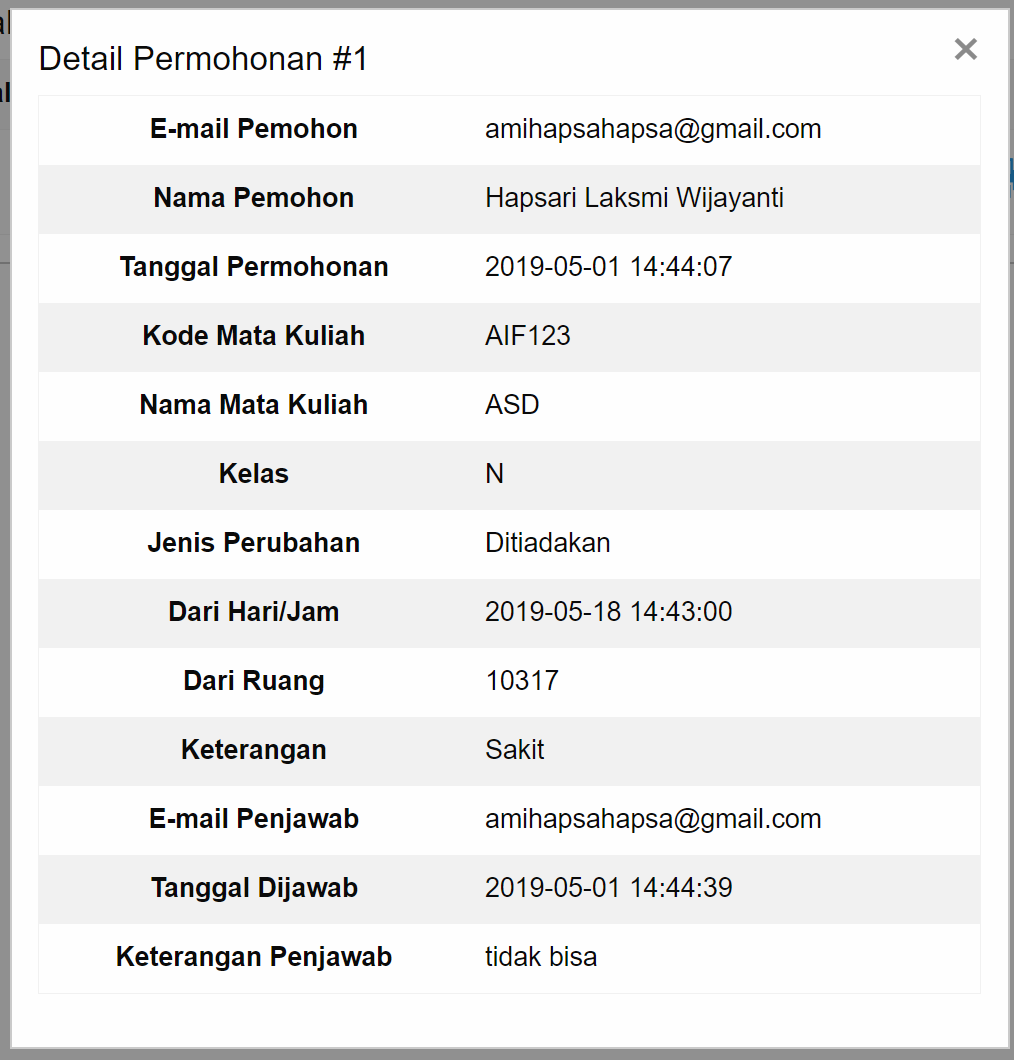
\includegraphics[scale=0.3]{Modal-Lihat-Manajemen-Perubahan-Kuliah.png}  
			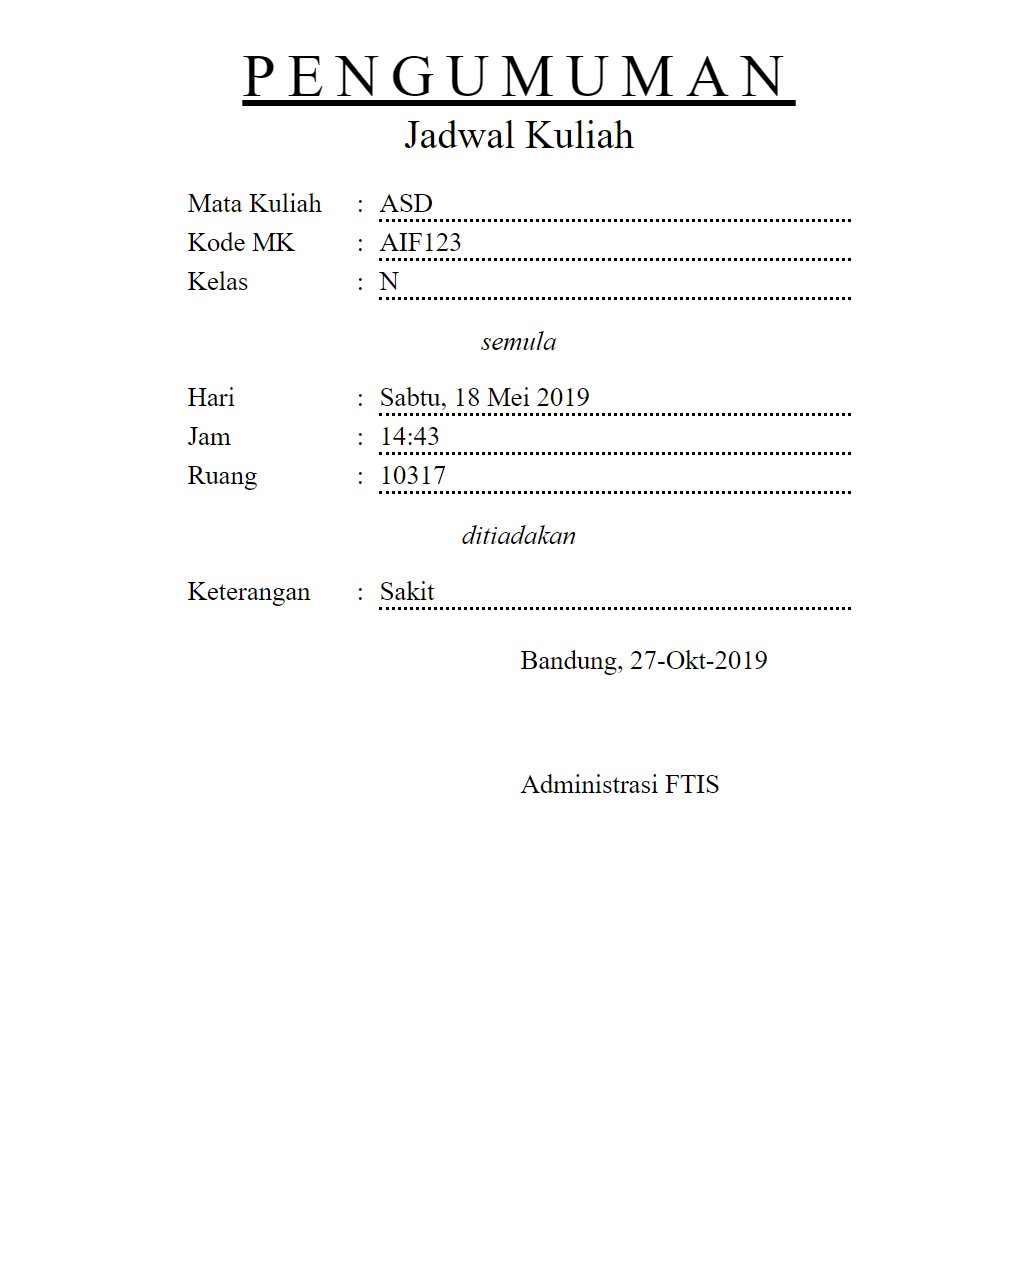
\includegraphics[scale=0.3]{Modal-Print-Manajemen-Perubahan-Kuliah.png} 
			\caption{Modal aksi Lihat dan Print Manajemen Perubahan Kuliah} 
		\end{figure}
		
		
		\begin{figure} [H]
			\centering  
			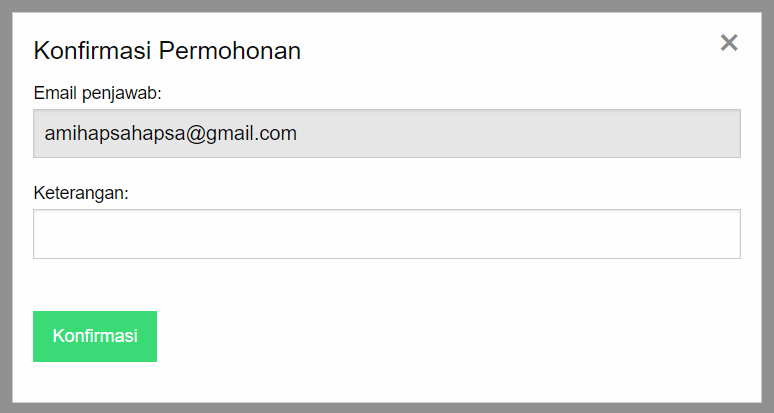
\includegraphics[scale=0.3]{Modal-Setuju-Manajemen-Perubahan-Kuliah.png}
			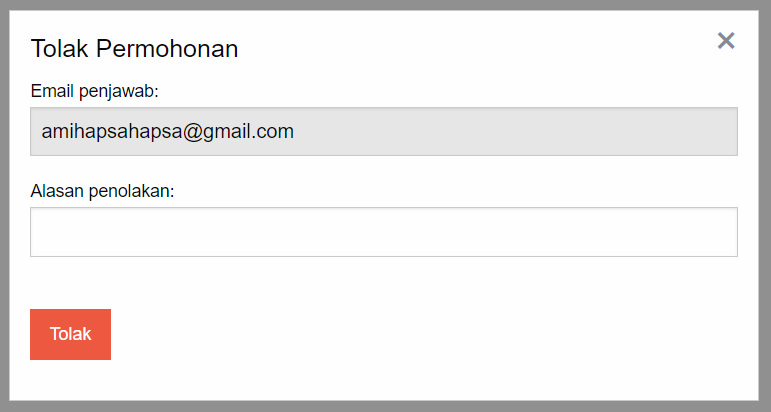
\includegraphics[scale=0.3]{Modal-Tolak-Manajemen-Perubahan-Kuliah.png}    
			\caption{Modal aksi Setuju dan Tolak Manajemen Perubahan Kuliah} 
		\end{figure}
		
		
		\begin{figure} [H]
			\centering  
			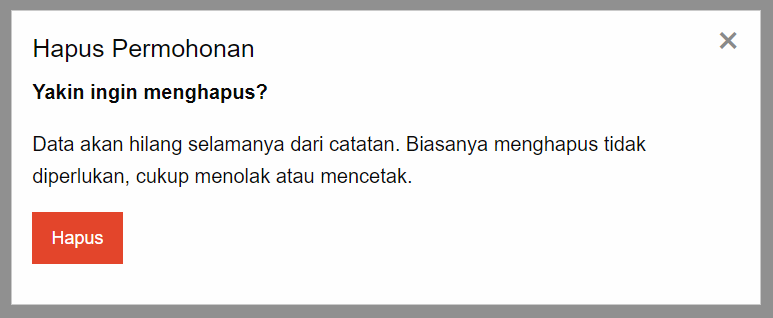
\includegraphics[scale=0.3]{Modal-Hapus-Manajemen-Perubahan-Kuliah.png}  
			\caption{Modal Hapus Manajemen Perubahan Kuliah} 
		\end{figure}
		
		Berikut ini penjelasan masing - masing modal.
		\begin{enumerate}
			
			\item Modal Lihat : Terdiri dari sebuah tabel yang menampilkan data tabel permohonan. Ikon menggunakan kelas  \colorbox{mygray}{\texttt{fi-eye}} dan menerapkan atribut  \colorbox{mygray}{\texttt{data-open}} yang berisi method hapus menuju ID tertentu.
			
			\item Modal Print : Terdiri dari sebuah form yang terdiri dari label, field dan tombol berwarna biru sehingga membutuhkan kelas  \colorbox{mygray}{\texttt{input-group-field}}.Ikon menggunakan kelas  \colorbox{mygray}{\texttt{fi-print}} dan menerapkan atribut \texttt{data-open} yang berisi method cetak menuju ID tertentu.
			
			\item Modal Setuju : Terdiri dari sebuah \texttt{table} yang menampilkan data permintaan transkrip. Ikon menggunakan kelas  \colorbox{mygray}{\texttt{fi-eye}} dan menerapkan atribut  \colorbox{mygray}{\texttt{data-open}} yang berisi method hapus menuju ID tertentu.
			
			\item Modal Tolak : Terdiri dari sebuah \textit{form} yang memiliki method \texttt{POST} yang memanggil sebuah method "/TranskripManage/answer". Terdapat tiga tipe input yang digunakan yaitu  \colorbox{mygray}{\texttt{hidden, text, submit}}. Pada input text untuk label Alasan Penolakan, menggunakan kelas "input-group-field". Lalu untuk input bertipe  \colorbox{mygray}{\texttt{submit}} menggunakan kelas alert-button untuk membuat button berwarna merah. Ikon menggunakan kelas \texttt{fi-dislike} dan menerapkan atribut  \colorbox{mygray}{\texttt{data-open}} yang berisi method tolak menuju ID tertentu.	
			
			\item Modal Hapus : Terdiri dari sebuah form yang terdiri dari paragraf yang bersifat bold, beberapa input dan tombol berwarna merah sehingga membutuhkan kelas \colorbox{mygray}{\texttt{<p>}}, \colorbox{mygray}{\texttt{<strong>}} dan \colorbox{mygray}{\texttt{<input>}}. Ikon menggunakan kelas  \colorbox{mygray}{\texttt{fi-trash}} dan menerapkan atribut \colorbox{mygray}{\texttt{data-open}} yang berisi method hapus menuju ID tertentu.
		\end{enumerate}
		
		\myparagraph{Antarmuka Entri Jadwal Dosen}
		Antarmuka diaplikasikan pada file \textbf{BlueTape/www/application/views/EntriJadwalDosen/main.php}.
		\begin{figure} [H]
			\centering  
			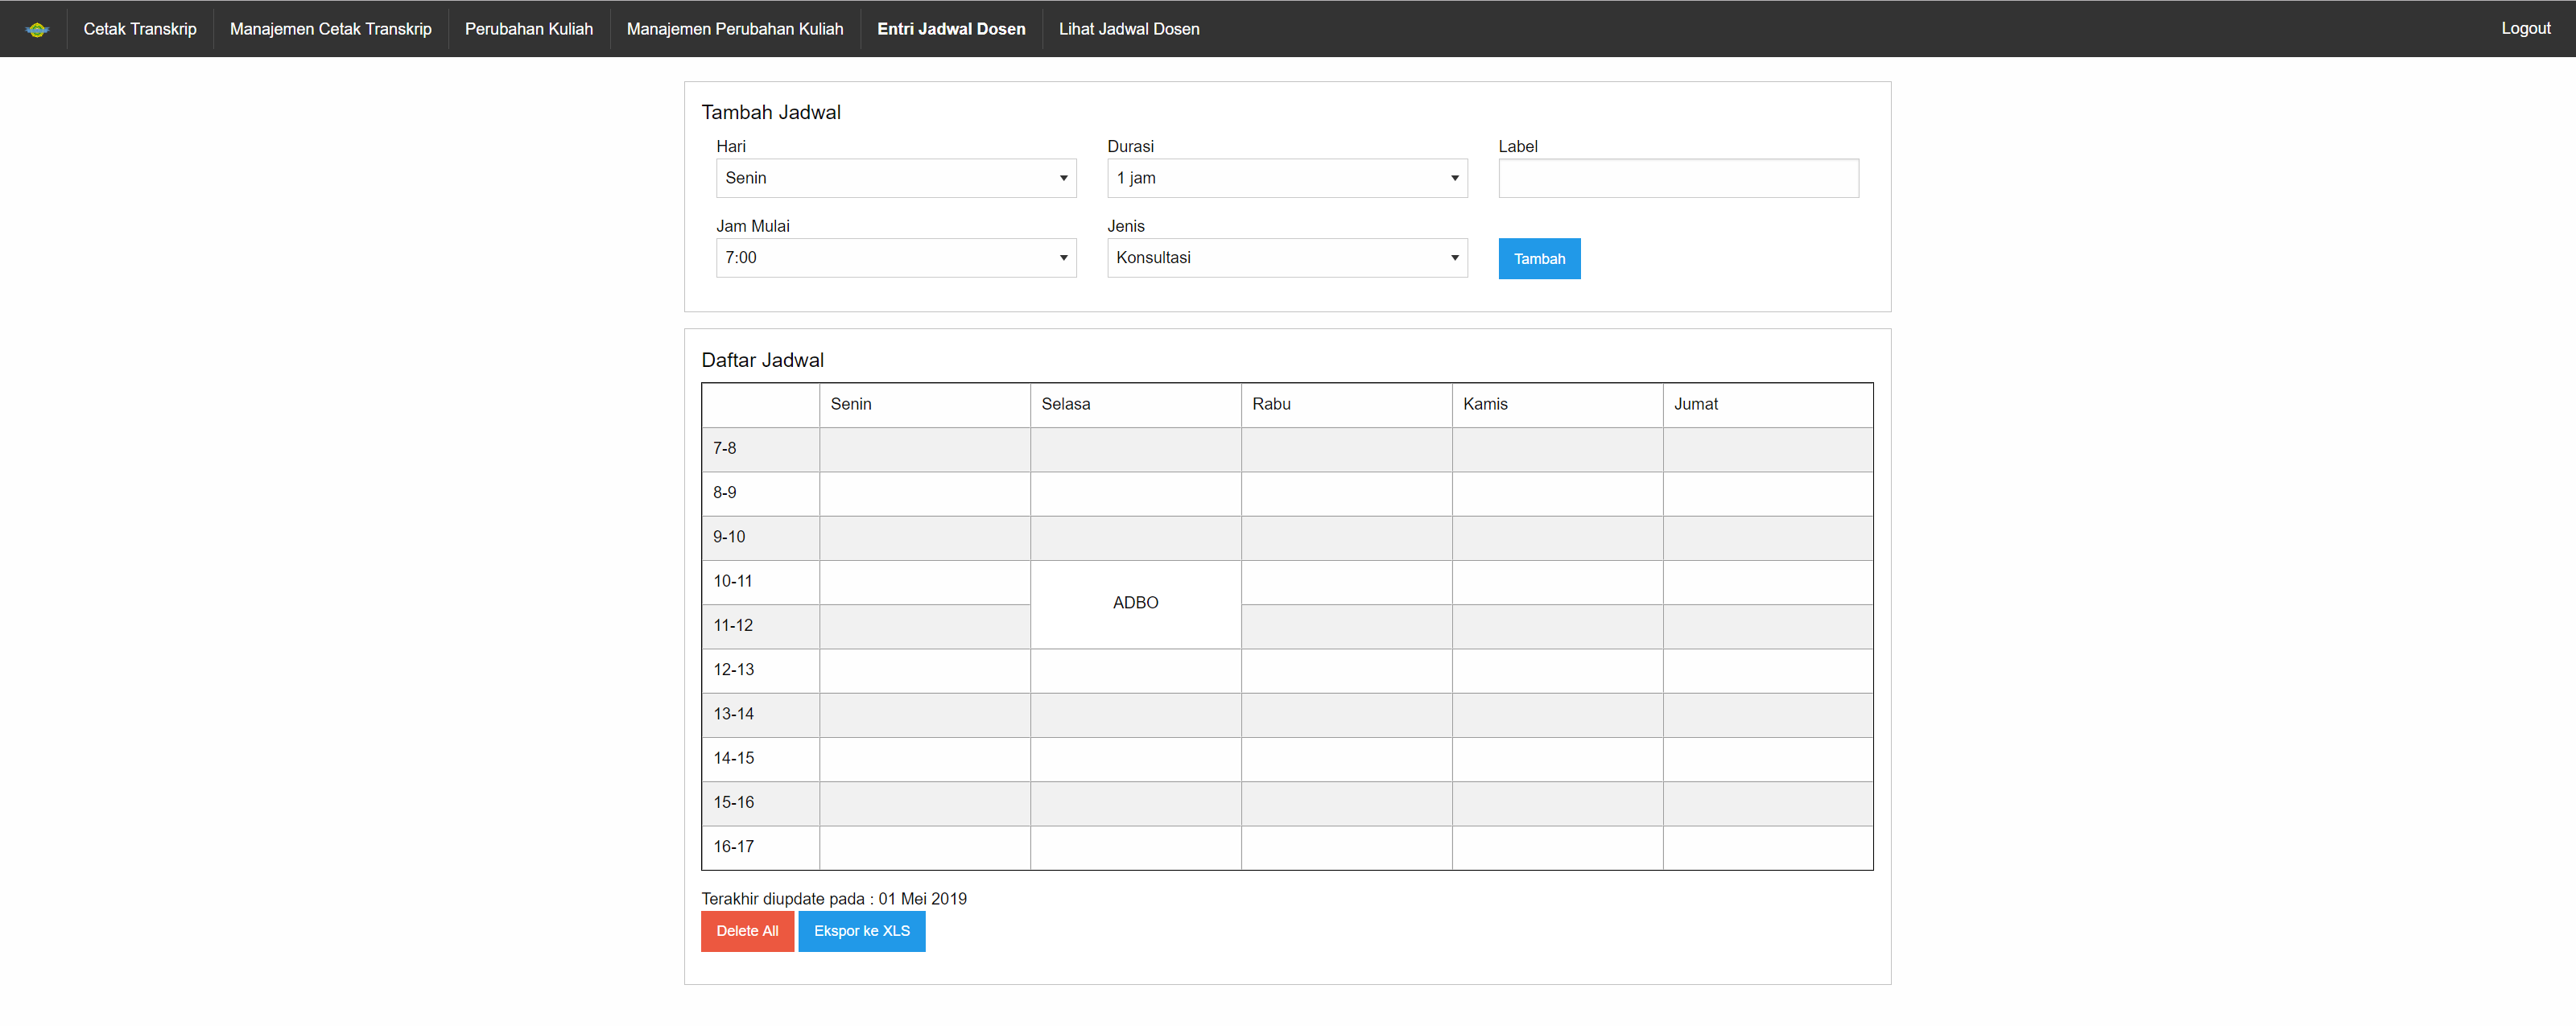
\includegraphics[scale=0.5]{Tampilan-Entri-Jadwal-Dosen.png}  
			\caption{Modal Print Manajemen Perubahan Kuliah} 
		\end{figure}
		
		Detail mengenai tabel Tambah Jadwal :
		\begin{itemize}
			\item \texttt{Hari} : Terdiri dari nama hari dari senin sampai jumat.
			\item \texttt{Durasi} : Terdiri dari rentang jam kelas berlangsung dari 1 jam hingga 9 jam.
			\item \texttt{Label} : Field bertipe text.
			\item \texttt{Jam Mulai} : Terdiri dari jam dari rentang 07:00 sampai 16:00.
			\item \texttt{Jenis} : Terdiri dari tiga macam pilihan 
			\begin{enumerate}
				\item Konsultasi : Memiliki background berwarna hijau.
				\item Terjadwal : Memiliki background berwarna biru.
				\item Kelas : Memiliki background putih.
			\end{enumerate}
		\end{itemize}
		
		Desain antarmuka sebagai berikut : \par
		Konten "Tambah Jadwal" dan "Daftar Jadwal" akan diletakkan pada satu \textit{row} yang memiliki kolom sebesar 12 grid pada layar medium dengan menggunakan komponen \colorbox{mygray}{\texttt{large-12 column}}, untuk setiap konten nya akan dipisahkan oleh panel yang disebut dengan \colorbox{mygray}{\texttt{callout}}. \par
		Untuk konten \texttt{Tambah Jadwal} :
		\begin{itemize}
			\item \texttt{Hari} : Penggunaan tag \colorbox{mygray}{\texttt{<select>}} dan \colorbox{mygray}{\texttt{<option>}}.
			\item \texttt{Jam Mulai} : Penggunaan tag \colorbox{mygray}{\texttt{<select>}} dan \colorbox{mygray}{\texttt{<option>}}.
			\item \texttt{Durasi} : Penggunaan tag \colorbox{mygray}{\texttt{large-4 columns}}
		\end{itemize}
		
		
		Tabel Daftar jadwal akan \textit{retrieve} data jadwal dari dosen yang dibuat. Terdiri dari rentang waktu dan hari. Jadwal yang terlihat pada tabel ini bisa diedit dan dihapus. Menggunakan kelas \colorbox{mygray}{\texttt{large-12 column}}, \colorbox{mygray}{\texttt{.callout}} dan \texttt{table-scroll}.
		Dibagian bawah tabel akan terlihat tanggal jadwal tersebut di update dan memiliki dua tombol :
		\begin{itemize}
			\item \texttt{Delete All} : Menghapus semua jadwal yang sudah dibuat, tombol berwarna merah dengan menerapkan kelas \colorbox{mygray}{\texttt{.alert}}.
			\item \texttt{Export ke XLS} : Secara otomatis akan membuat file excel dan mendownload di device secara lokal.Ttombol berwarna biru dengan menerapkan kelas \texttt{button}.
		\end{itemize}
		Setiap data yang ditampilkan bisa diedit atau hapus, apabila ditekan maka sebuah modal akan muncul.  
		\begin{figure} [H]
			\centering  
			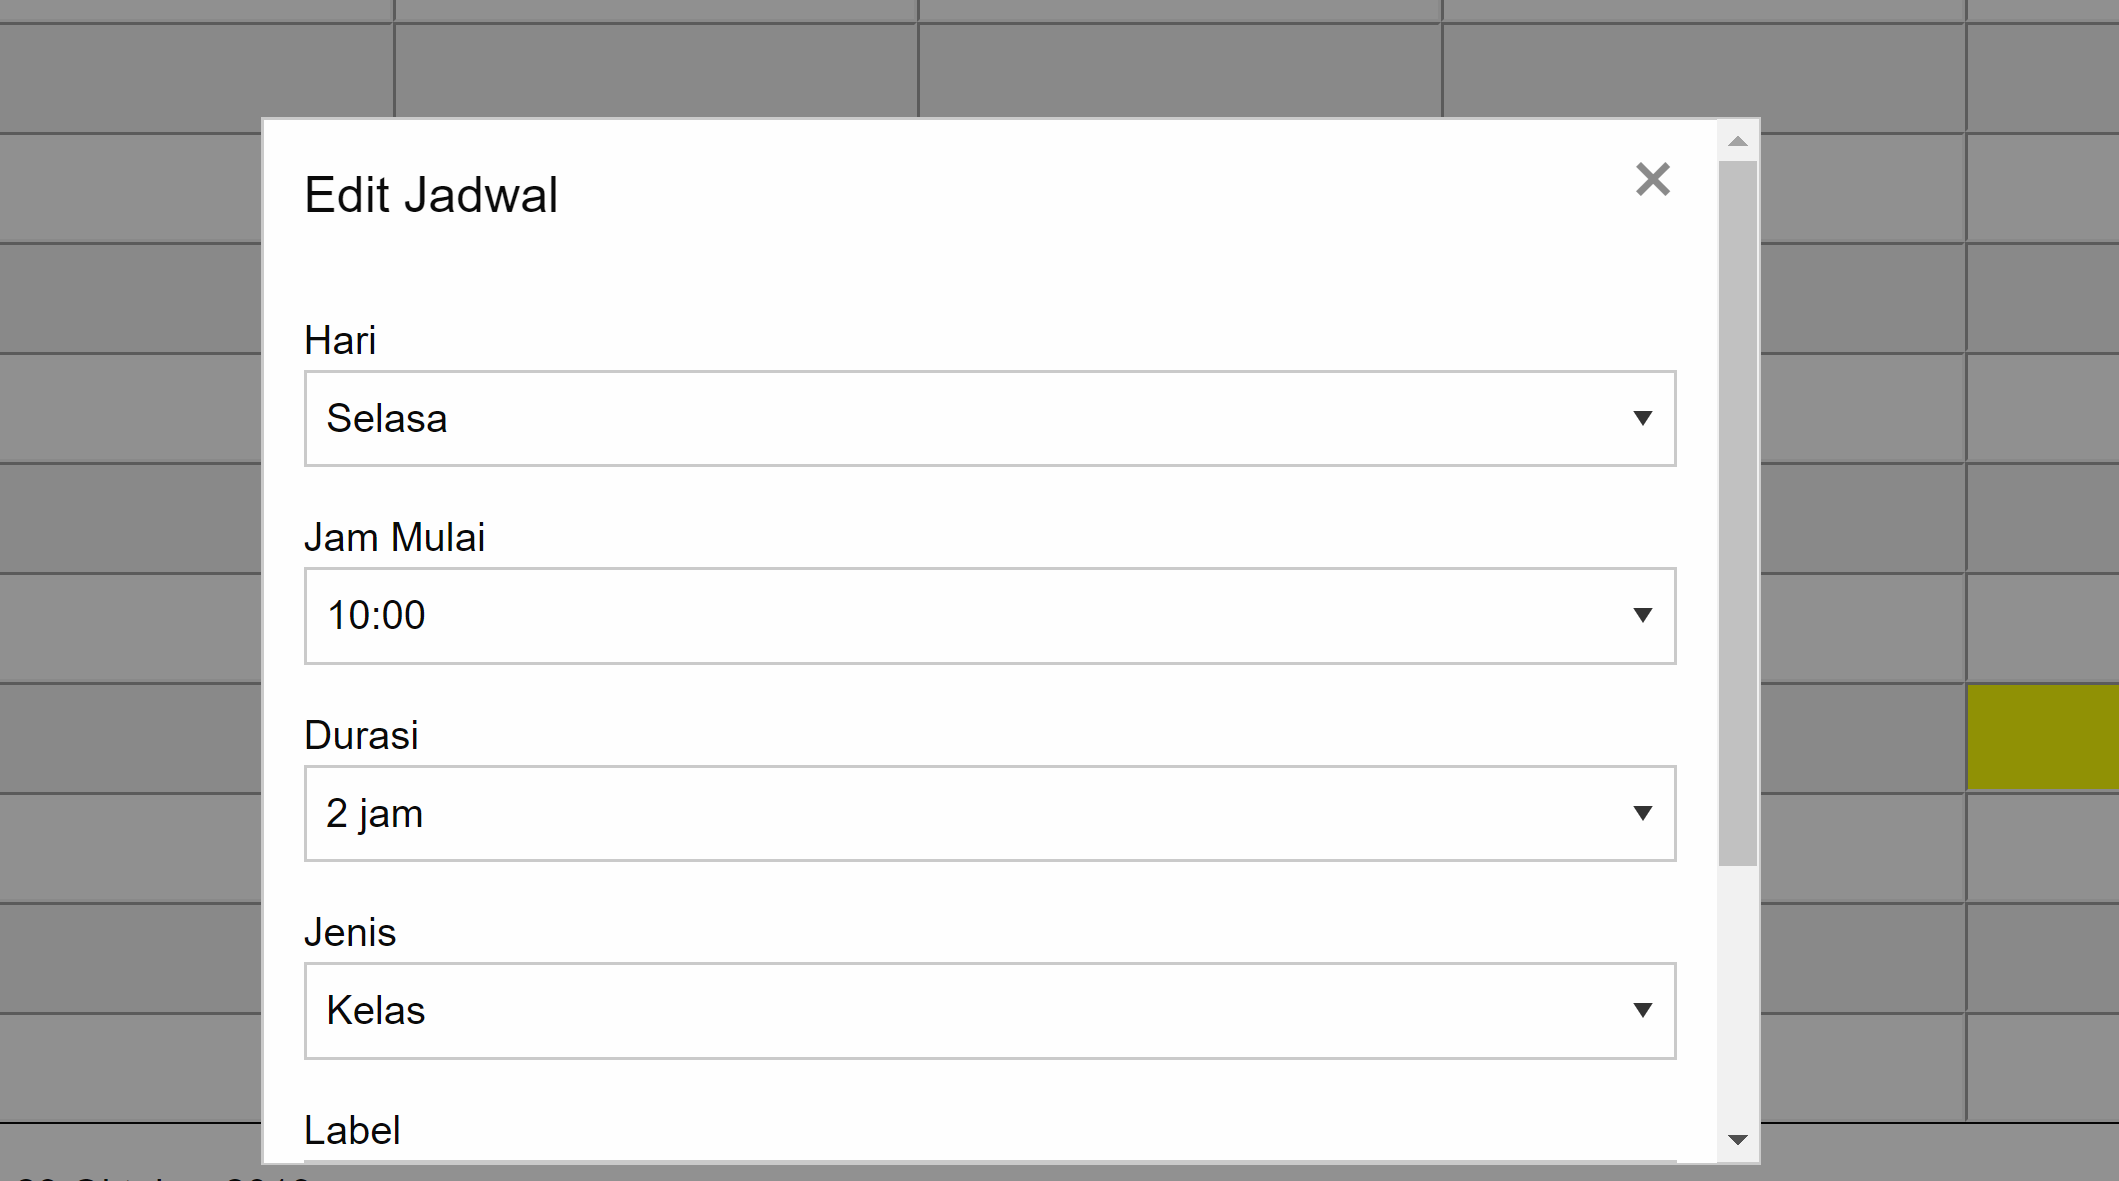
\includegraphics[scale=0.5]{Modal-Daftar-Jadwal-zurb.png}  
			\caption{} 	
		\end{figure}
		Modal merupakan sebuah form dengan metode "POST". Untuk field \texttt{Hari, Jam Mulai, Durasi, Jenis} dan \texttt{label} memiliki input bertipe \colorbox{mygray}{\texttt{select}}. Lalu terdapat dua button \texttt{Save} dan \texttt{Submit} yang masing - masing menggunakan kelas tag \colorbox{mygray}{\texttt{<button>}} dan \colorbox{mygray}{\texttt{.alert}}.
		
		\myparagraph{Antarmuka Lihat Jadwal Dosen}
		Antarmuka diaplikasikan pada file \textbf{BlueTape/www/application/views/LihatJadwalDosen/main.php}.
		\begin{figure} [H]
			\centering  
			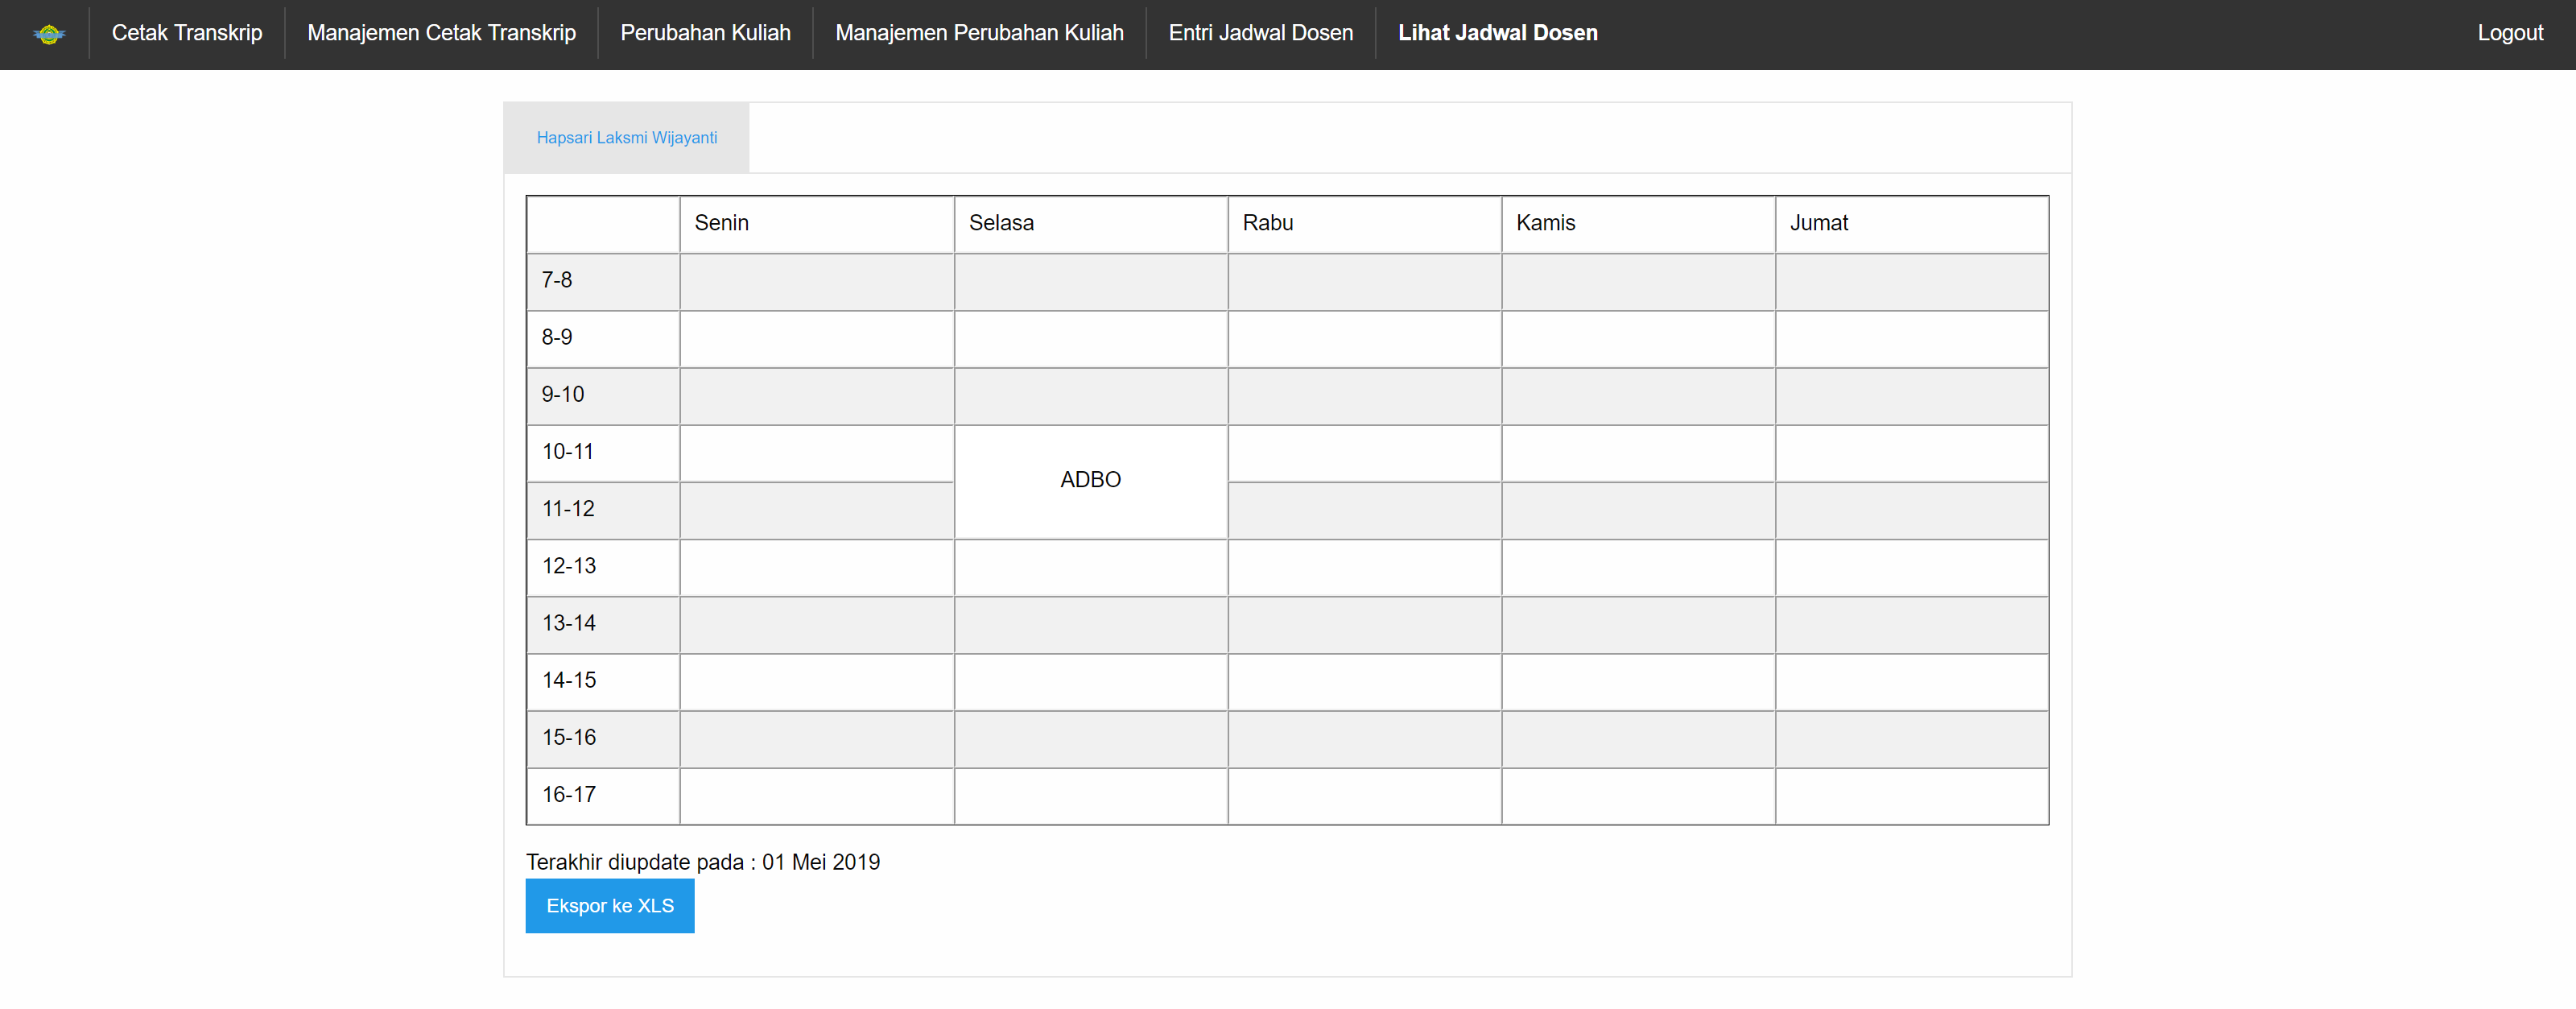
\includegraphics[scale=0.5]{Tampilan-Lihat-Jadwal-Dosen.png}  
			\caption{Struktur File Zurb Foundation} 	
		\end{figure}
		Tabel Jadwal Dosen terdiri dari list nama dosen yang dibuat dalam bentuk tabs sehingga menggunakan kelas \colorbox{mygray}{\texttt{tabs-panel}}. Apabila dipilih sebuah tabs maka tabel akan menampilkan data jadwal dosen.  Terdiri dari rentang waktu dan hari. Dibagian bawah tabel terdapat tanggal kapan terakhir jadwal dibuat dan tombol "Ekspor ke XLS".
		
		
		\item \textbf{Menulis dokumen skripsi.}\\
		{\bf Status :} Masih dalam pengerjaan. \\
		{\bf Hasil :}  Sudah mencapai bab 3.\\
		
		\section{Pencapaian Rencana Kerja}
		Langkah-langkah kerja yang berhasil diselesaikan dalam Skripsi 1 ini adalah sebagai berikut:
		\begin{enumerate}
			\item Mempelajari framework PHP Codeigniter.
			\item Mempelajari framework front-end Bootstrap 4 beserta plugin-plugin yang tersedia.
			\item Mengimplementasikan sebagian besar framework front-end Bootstrap 4 beserta plugin-plugin yang tersedia.
			\item Menulis dokumen skripsi.
		\end{enumerate}
		
		\section{Kendala yang Dihadapi}
		%TULISKAN BAGIAN INI JIKA DOKUMEN ANDA TIPE A ATAU C
		Kendala - kendala yang dihadapi selama mengerjakan skripsi :
		
		\vspace{1cm}
		\centering Bandung, \tanggal\\
		\vspace{2cm} \nama \\ 
		\vspace{1cm}
		
		Menyetujui, \\
		\ifdefstring{\jumpemb}{2}{
			\vspace{1.5cm}
			\begin{centering} Menyetujui,\\ \end{centering} \vspace{0.75cm}
			\begin{minipage}[b]{0.45\linewidth}
				% \centering Bandung, \makebox[0.5cm]{\hrulefill}/\makebox[0.5cm]{\hrulefill}/2013 \\
				\vspace{2cm} Nama: \pembA \\ Pembimbing Utama
			\end{minipage} \hspace{0.5cm}
			\begin{minipage}[b]{0.45\linewidth}
				% \centering Bandung, \makebox[0.5cm]{\hrulefill}/\makebox[0.5cm]{\hrulefill}/2013\\
				\vspace{2cm} Nama: \pembB \\ Pembimbing Pendamping
			\end{minipage}
			\vspace{0.5cm}
		}{
			% \centering Bandung, \makebox[0.5cm]{\hrulefill}/\makebox[0.5cm]{\hrulefill}/2013\\
			\vspace{2cm} Nama: \pembA \\ Pembimbing Tunggal
		}
	\end{document}
	
